\documentclass[bsc,letterpaper,12pt]{csthesis}
%\documentclass[letterpaper,12pt,twoside]{csthesis} % para imprimir de lado y lado


\paperwidth = 21.6cm		% Tamaño de la hoja
\paperheight = 27.9cm

%Margenes horizontales
\hoffset = -2.54cm		% Se elimna el offset horizontal
\oddsidemargin = 4cm
\evensidemargin = 2cm
\textwidth = 15.6cm

%Margenes verticales
\voffset = -2.54cm
\topmargin = 3cm
\headheight = 0cm
\headsep = 0cm
\textheight = 21.9cm
\footskip = 1cm


\usepackage[spanish,USenglish]{babel}     % Idioma Capitulos y demas
\usepackage[utf8]{inputenc}
\usepackage{lmodern}
\usepackage[T1]{fontenc}
\usepackage{cc/CreativeCommons}  %Licencia

\usepackage{listings} % Ingresar Codigo Fuente
\usepackage{verbatim}
\usepackage{moreverb}
\let\verbatiminput=\verbatimtabinput
\def\verbatimtabsize{8}  % Tabulación en verbatim

% Paquete para el manejo de hipervinculos
\usepackage[b5paper, breaklinks=true, pdfborder={0 0 0},colorlinks=false,pageanchor=true, 
plainpages=false,bookmarksopen=true,bookmarksopenlevel=3, hyperfootnotes=false]{hyperref}

% Paquete para el manejo de tablas
\usepackage{supertabular}

% Paquetes para simbolos
%\usepackage{mathcomp}
\usepackage{latexsym}
\usepackage{pifont}
\usepackage{amsfonts}
\usepackage{amssymb}
\usepackage{wasysym}
\usepackage{colortbl}
\usepackage{multicol} 
\usepackage{booktabs}
\usepackage{multirow}
\usepackage{algorithmic}
\usepackage[Algoritmo]{algorithm}
\usepackage{subfigure}

\usepackage{graphicx, wrapfig, lscape, rotating, float, booktabs}
\usepackage{tabularx}
\usepackage{longtable}
%\usepackage[backend=biber]{biblatex}


% Manejo de imagenes PDF y EPS
\newif\ifpdf
\ifx\pdfoutput\undefined
\pdffalse % we are not running PDFLaTeX
\else
\pdfoutput=1 % we are running PDFLaTeX
\pdftrue
\fi

\ifpdf
\usepackage[pdftex]{graphicx}
\else
\usepackage{graphicx}
\fi

\ifpdf
\DeclareGraphicsExtensions{.pdf, .jpg, .tif, .png, .JPG}
\else
\DeclareGraphicsExtensions{.eps, .jpg}
\fi
\graphicspath{{pictures/}} %En qué carpeta están las imágenes
% Sangria de comienzo de parrafo
\setlength{\parindent}{0cm}
% Espacio vertical entre dos parrfos
\setlength{\parskip}{0.3cm}

% Definir el nombre de listas
\addto\captionsspanish{%
  \def\prefacename{Prefacio}%
  \def\refname{REFERENCIAS}%
  \def\abstractname{RESUMEN}%
  \def\bibname{REFERENCIAS}%
  \def\chaptername{Cap\'{\i}tulo}%
  \def\appendixname{Anexo}%
  \def\listfigurename{Lista de figuras}%
  \def\listtablename{Lista de cuadros}%
  \def\indexname{\'Indice alfab\'etico}%
  \def\figurename{Figura}%
  \def\tablename{Tabla}%
  \def\partname{Parte}%
  \def\enclname{Adjunto}%
  \def\ccname{Copia a}%
  \def\headtoname{A}%
  \def\pagename{P\'agina}%
  \def\seename{v\'ease}%
  \def\alsoname{v\'ease tambi\'en}%
  \def\proofname{Demostraci\'on}%
  \def\glossaryname{Glosario}}
  \addto\captionsspanish{\def\contentsname{CONTENIDO}}
  
\addto\captionsUSenglish{
  \def\abstractname{ABSTRACT}%
}  


%para rotar tablas  
\usepackage{rotating}



%partir palabras
\hyphenation{di-fe-ren-cia pro-pues-to pro-ble-mas po-pu-la-res cons-truccio-nes ne-ce-sa-ria-men-te}

% Inico del documento
\begin{document}
\selectlanguage{spanish}
\pagestyle{empty}% Sin número de página
%%% PORTADA


\thispagestyle{empty}
\vspace*{1 mm}
\begin{center}{\centering \large Aplicación de técnicas de minería de texto  para el descubrimiento de relaciones conceptuales
entre los trabajos de grado de la Universidad de Nariño}
\end{center}

\vspace{2.5cm}

\begin{center}{\large Jimmy Mateo Guerrero Restrepo}
\end{center}

\vspace{1.5cm}

\begin{figure}[!h]
\begin{center}

\includegraphics[scale=0.7]{pictures/uba.png}%logo of your university
\end{center}
\end{figure}

\vspace{3.5cm}

\begin{center}{\large Universidad de Buenos Aires\\
Facultad de Ciencias Exactas y Naturales\\
Departamento de Computación\\
Maestría Explotación de Datos y Descubrimiento del Conocimiento\\
Buenos Aires Argentina\\
2020}
\end{center}



\pagebreak

\newpage

% CONTRAPORTADA

\thispagestyle{empty}

\vspace*{1 mm}
\begin{center}{\centering \large Aplicación de técnicas de minería de texto  para el descubrimiento de relaciones conceptuales
entre los trabajos de grado de la Universidad de Nariño}
\end{center}

\vspace{2.5cm}

\begin{center}{\large Jimmy Mateo Guerrero Restrepo}
\end{center}

\vspace{1cm}

\begin{center}
{\large Tesis presentada para optar al título de
{ Magíster de la Universidad de Buenos Aires en Explotación de Datos y Descubrimiento del Conocimiento}}
\end{center}

\vspace{1cm}

\begin{center}
{\large DIRECTOR:  Ricardo Timaran Pereira, PhD} 
\end{center}

\vspace{4.5cm}

\begin{center}{\large Universidad de Buenos Aires\\
Facultad de Ciencias Exactas y Naturales\\
Departamento de Computación\\
Maestría Explotación de Datos y Descubrimiento del Conocimiento\\
Buenos Aires Argentina\\
2020}
\end{center}

\pagebreak

%\chapter*{NOTA DE RESPONSABILIDAD}

``Las ideas y conclusiones aportadas en la tesis de grado, son 
responsabilidad exclusiva de sus autores''.

Articulo 1$\textordmasculine$ del acuerdo N$\textordmasculine$ 324 del 11 de octubre de 1966, 
emanado del 
Honorable Consejo Directivo de la Universidad de Nariño

``La Universidad de Nariño no se hace responsable de las opiniones o resultados obtenidos 
en el presente trabajo y para su publicación priman las normas sobre el derecho de autor''

Artículo 13, Acuerdo N. 005 de 2010 emanado del Honorable Consejo Académico.

\newpage
\vspace*{1 mm}
\begin{flushright}
Nota de aceptación:\linebreak \linebreak \linebreak 

\underline{\hspace{8cm}}\linebreak \linebreak
\underline{\hspace{8cm}}\linebreak \linebreak
\underline{\hspace{8cm}}\linebreak \linebreak
\underline{\hspace{8cm}}

\vspace{1cm}
\underline{\hspace{8cm}}\\
Firma del presidente del jurado \linebreak \linebreak \linebreak \linebreak \linebreak 

\underline{\hspace{8cm}}\\
Firma del jurado \linebreak \linebreak 

\vspace{1cm}
\underline{\hspace{8cm}}\\
Firma del jurado

\end{flushright}


\vspace{1cm}
San Juan de Pasto, 2014 


\newpage
\pagestyle{empty}
%\CCbysaInfo	%Licencia  Attribution-ShareAlike 3.0
%\CCbyInfo	%Creative Commons Attribution 3.0
%\CCbyndInfo	%Creative Commons Attribution-No-Derivs 3.0
\CCbyncInfo	%Creative Commons Attribution-Non-Commercial 3.0
%\CCbyncsaInfo	%Creative Commons Attribution-Non-Commercial-ShareAlike 3.0
%\CCbyncndInfo	%Creative Commons Attribution-Non-Commercial-NoDerivs 3.0



\chapter*{}
%pagenumbering{Roman} % para comenzar la numeracion de paginas en numeros romanos
\begin{flushright}
\textit{Dedicado a: \\
Mis padres quienes me han apoyado  para poder avanzar peldaño a peldaño a lo largo de mi vida.}

\textit{Mi hermana por brindarme su apoyo y compañía.}


\end{flushright}


\chapter*{AGRADECIMIENTOS} % si no queremos que añada la palabra "Capitulo"

Por encima de todo agradezco a Dios por haberme acompañado y guiado a lo largo de mis estudios de maestría, por ser mi fortaleza en mis momentos de debilidad y por brindarme una vida llena de cosas que aprender. GRACIAS TE DOY MI SEÑOR.

Agradezco a mis padres: JAIME GUERRERO Y OLMA LUZ RESTREPO por apoyarme en todos los momentos, por inculcarme valores que han hecho de mi una persona consciente de mi rol social. GRACIAS PADRES.

A mi hermana por ser parte de mi vida y representar la unidad familiar, llenar mi vida de alegría y felicidad cuando más la he necesitado.

A la gobernación de Nariño por financiar mis estudios, a través de la fundación Ceiba.

Le agradezco la confianza, apoyo, dedicación y  valiosa orientación de este trabajo   a  mi director Ricardo Timarán Pereria.
  
A todos los profesores de la maestría  por sus enseñanzas.   

A Omar Ernesto Cabrera, por ser un compañero que supo compartir su conocimiento y apoyarme en toda empresa educativa y de aprendizaje que emprendimos.
 
\selectlanguage{spanish}

\begin{abstract}


\textbf{Objetivo}: Descubrir relaciones conceptuales entre los trabajos de grado de la Universidad de Nariño (Colombia) utilizando técnicas de minería de texto que faciliten la recuperación de trabajos de grado relacionados con la temática de la búsqueda identificando similitudes y diferencias entre ellos. \textbf{Metodología}: Se utilizó CRISP-DM como metodología. Usando diferentes técnicas de minería de texto, tales como Bag (bolsa de palabras), Tf-Idf y Doc2vec se estructuraron los documentos del repositorio de trabajos de grado de la Universidad de Nariño. Se utilizaron técnicas de aprendizaje no supervisado para encontrar relaciones taxonómicas (también llamadas relaciones categoriales) en los documentos estructurados. Con el modelo de reconocimiento de entidades (NER) se descubrieron conceptos claves en los diferentes grupos encontrados, se entrenó el modelo  Word2vec para encontrar relaciones temáticas entre estos conceptos. Para inferir temas de búsqueda a cada categoría encontrada se entrenó varios modelos de aprendizaje supervisado, con los modelos entrenados se implementaron algoritmos en la herramienta Maskana  con el fin de encontrar documentos relacionados a temas de búsqueda. \textbf{Resultados}: Se encontró el número óptimo de relaciones categoriales, con la implementación de los algoritmos se logró interpretar los conceptos de cada categoría y sus relaciones,  las pruebas demostraron que el modelo Doc2vec es el más adecuado para la estructuración del corpus de trabajos de grado,
el modelo Xgboost resultó superior a los demás clasificadores; este modelo permite clasificar nuevos documentos que ingresen al repositorio y se implementó en el algoritmo \ref{alg:maskanita1}; para clasificar temáticas de búsqueda en las categorías o grupos encontrados y con esto poder recuperar documentos similares a esta. 
 \textbf{Conclusiones}: Se descubrieron relaciones conceptuales en los trabajos de grado de  la Universidad de Nariño; al utilizar técnicas de minería de texto que facilitaron la recuperación de trabajos relacionados en las temáticas de búsqueda, identificando similitudes y diferencias entre ellos.


%
% Las pruebas demostraron que el modelo Doc2vec es el más adecuado para la estructuración del corpus de trabajos de grado. El número óptimo de categorías o grupos de conocimiento es 32. El modelo Xgboost resultó superior a los demás clasificadores; este modelo permite clasificar nuevos documentos que ingresen al repositorio y se implementó en el algoritmo \ref{alg:maskanita1}; para clasificar temáticas de búsqueda en las categorías o grupos encontrados y con esto poder recuperar documentos similares a esta. 

%Los modelos Ner y Word2vec permitieron interpretar el conocimiento relacionado a cada una de las categorías encontradas, lo cuales fueron implementados en el algoritmo \ref{alg:maskanita2}; el cual visualiza relaciones conceptuales temáticas entre los documentos del repositorio


\textbf{Palabras clave:} minería de textos; relaciones conceptuales; aprendizaje automático; NER, Word2vec, Doc2vec.
\end{abstract}


\selectlanguage{USenglish}

\begin{abstract}
\textbf {Objective}: To discover conceptual relationships between undergraduate projects at the University of Nariño (Colombia) using text mining techniques that facilitate the retrieval of undergraduate projects related to the topic of the search, identifying similarities and differences between them. \textbf {Methodology}: CRISP-DM was used as methodology. Using different text mining techniques, such as Bag (bag of words), Tf-Idf and Doc2vec, the documents of the repository of degree works of the University of Nariño were structured. Unsupervised learning techniques were used to find taxonomic relationships (also called categorical relationships) in the structured documents. With the entity recognition model (NER), key concepts were discovered in the different groups found, the Word2vec model was trained to find thematic relationships between these concepts. To infer search topics for each category found, several supervised learning models were trained, with the trained models algorithms were implemented in the Maskana tool in order to find documents related to search topics. \textbf {Results}: The optimal number of categorical relationships was found, with the implementation of the algorithms it was possible to interpret the concepts of each category and their relationships, the tests showed that the Doc2vec model is the most appropriate for structuring the corpus of degree works,
the Xgboost model was superior to the other classifiers; This model allows classifying new documents that enter the repository and was implemented in the algorithm \ref {alg:maskanita1}; to classify search topics in the categories or groups found and thus be able to retrieve documents similar to this one.
\textbf {Conclusions}: Conceptual relationships were discovered in the degree projects of the University of Nariño; by using text mining techniques that facilitated the recovery of related works in the search topics, identifying similarities and differences between them.

\textbf{Keywords:}text mining; conceptual relationships; machine learning; NER, Word2vec, Doc2vec.
\end{abstract}
 

\selectlanguage{spanish}
\tableofcontents
%\chapter*{ACRÓNIMOS}
 
\begin{description}
 \item [BFE] Basic Flock Evaluation
 \item [CAD] Computer Aided Design
 \item [DBMS] Database Management System
 \item [FPFLock] Frequent Pattern Flock
 \item [GPS] Global Positioning System
 \item [LCM] Linear time Closed itemset Miner
 \item [LCMFlock]  Linear time Closed item set Miner Flock
 \item [MOD] Moving Objects Databases
 \item [RFID] Radio Frequency IDentification
  \item [SUMO] Simulation of Urban MObility
 \item [VLSI]  Very Large Scale Integration
\end{description}

\chapter*{INTRODUCCIÓN}
\addcontentsline{toc}{chapter}{INTRODUCCIÓN}
\\

La minería de texto ha despertado un enorme interés en la comunidad científica, ya que ha aumentado su auge enormemente en los últimos años debido a la creciente cantidad de documentos disponibles en formato digital, y también a la creciente necesidad de organizar y obtener el conocimiento contenido en textos.
La literatura en el campo de la minería de textos ofrece una serie amplia de aplicaciones tales como la clasificación supervisada, la recuperación de información , la clasificación no supervisada (CNS) , extracción de entidades con nombre (NER), encontrar tendencias mediante nubes de palabras, extraer resúmenes de grandes volúmenes de texto, La mayoría de las técnicas propuestas en este ámbito se basan en el paradigma del aprendizaje artificial \cite{sebastiani2002machine}. Un pilar importante de la minería de textos es la representación de documentos no estructurados de tal forma que reflejen los distintos rasgos de su contenido de la mejor manera posible. Esto es sumamente importante cuando se trabaja con colecciones de documentos no etiquetados mediante una clase, como los que se trata en este proyecto denominados problemas de CNS \cite{jain2010data}.

%\textbf{Planteamiento del problema}
En el proceso investigativo realizado en el Grupo de Investigación Aplicada en Sistemas -  GRIAS (\textcolor{Cyan}{\underline{\url{http://grias.udenar.edu.co/grias/}}})
, en  la  línea  de  
investigación  de  Herramientas  y  Sistemas  de  Gestión  de Conocimiento  y  Recuperación  de  Información,
se  han  desarrollado  dos  proyectos  de investigación financiados por el sistema de investigaciones de la Universidad de Nariño: uno
por  la  convocatoria  estudiantil  denominado  ''Construcción  de  una  Ontología  de Aplicación  que  Soporte 
la  Búsqueda  Inteligente  sobre  los  Trabajos  de  Grado  de  la Universidad  de  Nariño  denominada  SAWA,  utilizando 
la  herramienta  de  software  libre Protégé'' \cite{cabrera2015swa} y otro en la convocatoria de trabajos de grado denominado
''UMAYUX: Un Modelo de Software de Gestión de Conocimiento Soportado en una Ontología Dinámica Débilmente Acoplado con un 
Gestor de Bases de Datos para la Universidad de Nariño'' \cite{benavides2014umayux}.  Estos  proyectos  fueron  delimitados  a  los  trabajos  de  grado 
del  programa  de Ingeniería de Sistemas de la Universidad de Nariño. Como resultado de estos proyectos se  cuenta  con  "MASKANA"  \cite{restrepo2015maskana}, 
un  prototipo  de  gestor  documental  para  recuperación  de información  relacionada  con 
los  trabajos  de  grado  del  programa  de  Ingeniería  de Sistemas  almacenados  en  formato  digital.  En estos proyectos se dispone 
de un repositorio textual de documentos no estructurados sin etiqueta de  clase, el cual se limito a encontrar relaciones semánticas
sin tener en cuenta los conceptos y NER.

Segun Vivas, Leticia y Coni, Ana Gar  \cite{VIVAS2013}, "los conceptos son elementos esenciales para el reconocimiento del mundo que nos rodea. Ellos constituyen una representación de una clase de cosas. Frecuentemente, se suelen confundir o utilizar indistintamente los términos concepto y palabra. El concepto [escuela],
por ejemplo, debe ser distinguido de la palabra 'escuela'. [Escuela] es un tipo de [institución educativa]. El concepto [escuela] puede,
por ejemplo, ser expresado por las palabras 'escuela', 'lugar para educar', 'institución educativa'. 
Los conceptos están profundamente relacionados unos con otros de manera que la activación de unos genera la 
activación de otros. Los vínculos que los interconectan se denominan relaciones conceptuales. Este tipo de relaciones no debe 
ser confundido con las relaciones entre términos o palabras. Mientras que a las primeras se las suele denominar relaciones conceptuales,
a las segundas se las suele denominar relaciones semánticas. Por ejemplo, las relaciones de sinonimia o de homonimia son
relaciones semánticas, mientras que las relaciones taxonómicas y 
temáticas son relaciones primordialmente entre conceptos."

Para Estes, Zachary , Golonka, Sabrina y Jones, Lara  \cite{estes2011thematic},  "las relaciones taxonómicas (también llamadas relaciones categoriales) son las que vinculan a conceptos de una misma categoría semántica.
Los objetos de la misma categoría taxonómica usualmente comparten el nombre genérico.
Dado que los componentes de este tipo de relaciones tienen rasgos comunes, las vinculaciones se establecen principalmente mediante mecanismos de detección de similitudes, es decir, comparando las propiedades de ambos conceptos.
Este tipo de relaciones permiten, agrupar los conceptos de una misma categoría, anticipar, mediante procesos de deducción e inferencia, las propiedades que tendrá un nuevo elemento que se incluya dentro de la categoría."

De acuerdo a Golonka, Sabrina y Estes, Zachary \cite{golonka2009thematic}, "las relaciones temáticas, Son relaciones contextuales entre objetos que no son del mismo tipo pero que pueden ser encontrados en los mismos esquemas. Específicamente, una cosa está temáticamente relacionada con otra cuando ambas desempeñan roles complementarios en el mismo escenario o situación." 

Segun Barsalou, Lawrence \cite{barsalou2003grounding}, " las relaciones temáticas permiten organizar contextualmente la experiencia así como establecer predicciones frente a situaciones futuras similares mediante el mecanismo de inferencia de completamiento de patrones." 

Se han propuesto diferentes técnicas de minería de textos, en \cite{troyano2003identificacion} 
describen los enfoques de extracción de NER y conceptos ligados al conocimiento, en \cite{figuerola2004algunas}
aplican técnicas para extraer palabras clave de documentos textuales.
En \cite{llorens1998caracteristicas}, \cite{santana2014aplicacion}, \cite{barrera2016mineria} y \cite{rodriguez2018metodos}
proponen aplicar técnicas de minería de textos para representar documentos no estructurados,
en \cite{MONTESYGOMEZ2005} y  \cite{munozutilizacion}
usan grafos conceptuales como representación del contenido de los textos, y obtiene algunos patrones descriptivos de los documentos aplicando varios tipos de operaciones sobre estos grafos.

Estos antecedentes proponen diferentes alternativas de minería de textos pero ninguno de ellos aplicado al dominio de trabajos de grado. 

Esto implico  investigar diferentes técnicas de minería de textos y minería de datos, aplicarlas
en el repositorio, evaluar su correcto funcionamiento e interpretar los patrones obtenidos generando conocimiento
útil para el repositorio de la biblioteca Alberto Quijano Guerrero de la universidad de Nariño.


\textbf{Objetivos}
 
Esta investigación tuvo como objetivo  descubrir relaciones conceptuales entre los trabajos de grado de la Universidad de Nariño (Colombia)
utilizando técnicas de minería de texto que facilite la recuperación de trabajos de grado
relacionados con la temática de la búsqueda identificando  similitudes y diferencias  entre ellos.

Para alcanzar este objetivo se plantearon los siguientes objetivos específicos 

\begin{itemize}
\item Apropiar el conocimiento en algoritmos de minería de texto, algoritmos de agrupación  y aprendizaje automático.
\item Construir, limpiar y transformar  el repositorio de documentos de trabajos de grado de la universidad de Nariño.
\item Implementar los algoritmos de minería de texto seleccionados en la herramienta MASKANA.
\item Descubrir las relaciones conceptuales entre los trabajos de grado y evaluar los resultados.
\end{itemize}


Este documento está organizado de la siguiente manera: en el capítulo 1 se elabora un marco teórico referente a minería de textos, en el capítulo 2 se presenta la metodología, en el capítulo 3 se interpretan y discuten los resultados y finalmente  en el capítulo 4 se muestra las conclusiones y trabajos futuros en base a los resultados.
% \chapter{TRABAJOS RELACIONADOS}

Las capacidad de recolectar datos de objetos en movimiento ha ido aumentando 
rápidamente y el interés de consulta
de patrones que describen el comportamiento colectivo también ha aumentado. 
\cite{vieira2009line} enumera tres grupos de patrones
``colectivos'' en bases de datos de objetos en movimiento: clústers móviles, 
consulta de convoyes y patrones de agrupamiento.

Los clústers móviles \cite{jensen2007continuous} \cite{kalnis2005discovering} 
\cite{li2008mining} 
y  consultas de convoyes  \cite{jeung2008discovery-1} \cite{jeung2008convoy}, 
tienen en común que se basan en algoritmos
de clústering, principalmente en algoritmos basados en densidad como el 
algoritmo DBSCAN\cite{ester1996density}.

Los clústers móviles se definen entre dos instantes de tiempo consecutivos. Los 
clústers  se pueden unir sólo si el número de objetos comunes entre ellos están 
por encima del parámetro predefinido.
Un clúster es reportado si no hay otro nuevo clúster que pueda ser unido a éste. 
Este proceso se aplica cada vez para 
todos los instantes de tiempo en el conjunto de datos. 

Las consultas de convoyes se definen como un clúster denso de trayectorias que 
permanecen juntas al menos por un tiempo contínuo predefinido. 

Las principales diferencias entre las dos técnicas son la forma en que se unen 
los grupos  entre dos intervalos
consecutivos de tiempo y el uso de un parámetro adicional para especificar un 
tiempo mínimo de duración. Aunque
estos métodos están estrechamente relacionados con los patrones de agrupamiento, 
ninguno de ellos asume una  forma predefinida.

Previos trabajos de detección de patrones de agrupamiento móviles son descritos 
por \cite{ gudmundsson2006computing}
y \cite{benkert2008reporting}. Ellos introducen
el uso de discos con un radio predefinido para identificar  grupos de 
trayectorias que se mueven juntos en la misma
dirección, todas las trayectorias que se encuentran dentro del disco en un 
instante  de tiempo particular se 
considera un patrón candidato. La principal limitación de este proceso es que 
hay un número infinito de posibles
ubicaciones del disco en cualquier instante de tiempo. En efecto, en 
\cite{gudmundsson2006computing} se ha demostrado
que el descubrimiento de agrupaciones fijas, donde los patrones de las mismas 
entidades permanecen juntas durante 
todo el intervalo, es un problema NP-complejo. 

\cite{vieira2009line} son  los  primeros  en  presentar  una  solución  exacta  
para  reportar  patrones  de agrupación en tiempo polinomial, y también pueden trabajar efectivamente en 
tiempo real. Su trabajo revela que el tiempo de solución polinomial se puede encontrar 
a través de  la  identificación  de  un  número  discreto  de  ubicaciones  para  colocar 
 el  centro  del disco.  Los  autores  proponen  el  algoritmo  BFE  (Basic  Flock  Evaluation)  
basado  en  el tiempo de unión y combinación de los discos. La idea principal de este algoritmo 
es primero  encontrar  el  número  de  discos  válidos  en  cada  instante  de  
tiempo  y  luego combinarlos  uno  a  uno  entre  tiempos  adyacentes. Adicionalmente,  se  
proponen  otros cuatro  algoritmos  basados  en  métodos  heurísticos,  para  reducir  el  
número  total  de candidatos  a  ser  combinados  y,  por  lo  tanto,  el  costo  global del
algoritmo.  Sin  embargo,  el pseudocódigo y  los  resultados  experimentales
muestran todavía una alta complejidad computacional, largos tiempos de respuesta,
debido a que este algoritmo usa $\delta$ para partir los flocks hace que el número de patrones
encontrados sea mayor y esto hace difícil su interpretación.


\cite{romero2011mining} y \cite{turdu2014} proponen  una  metodología  que  
permite  identificar  patrones de agrupamiento utilizando tradicionales y potentes algoritmos de minería de datos 
usando patrones frecuentes, el cual fue comparado con BFE demostrando un alto 
rendimiento con conjuntos de datos sintéticos, aunque con conjuntos de datos reales el 
tiempo de respuesta siguió siendo eficiente pero similar a BFE. Este algoritmo trata el 
conjunto de trayectorias como una base de datos transaccional al convertir cada trayectoria, 
que se define  como  un  conjunto  de  lugares  visitados,  en  una  transacción,  
definida  como  un conjunto  de ítems.  De  esta  manera,  es  posible  aplicar  cualquier  
algoritmo  de  reglas  de asociación y encontrar patrones frecuentes sobre el conjunto dado, este algoritmo hace un llamado a LCM
propuesto por \cite{uno2004lcm} para encontrar patrones máximos y eso permite encontrar los flocks más largos.
\chapter{Fundamentos Teóricos}

% https://medium.com/analytics-vidhya/automated-keyword-extraction-from-articles-using-nlp-bfd864f41b34
% https://course.spacy.io/
% https://medium.com/qu4nt/reducir-el-n%C3%BAmero-de-palabras-de-un-texto-lematizaci%C3%B3n-y-radicalizaci%C3%B3n-stemming-con-python-965bfd0c69fa
% https://towardsdatascience.com/topic-modeling-and-latent-dirichlet-allocation-in-python-9bf156893c24
% https://medium.com/@datamonsters/text-preprocessing-in-python-steps-tools-and-examples-bf025f872908
% https://towardsdatascience.com/end-to-end-topic-modeling-in-python-latent-dirichlet-allocation-lda-35ce4ed6b3e0
% http://datamining.dc.uba.ar/datamining/files/Tesis/TesisGastonLiberman.pdf
% https://towardsdatascience.com/tf-idf-for-document-ranking-from-scratch-in-python-on-real-world-dataset-796d339a4089



\section{Minería de texto}

Se debe definir primero conceptos básicos que son clave para hablar de minería de textos 
como dato, información, conocimiento y minería de datos, para lograr un mejor entendimiento y
contextualizar al lector desde una primera instancia.

Dato es un conjunto discreto de valores, por ejemplo:  Mateo, Sistemas, 10 . Información es el conjunto de
datos procesados y que tienen un significado (relevancia, propósito y contexto) dado por el observador,
como puede ser, Mateo estudio 10 semestres   de ingeniería de sistemas. Luego, el conocimiento será la capacidad de
transformar la información y la experiencia de las personas en la toma de decisiones sobre una acción.
En el mundo de las tecnologías de la información, los datos son almacenados normalmente en bases de
datos y su volumen puede llegar a ser muy grande, a partir de esto surge la minería de datos para ayudar
a la comprensión de los contenidos en dicho almacenamiento. Las bases de datos tienen una estructura
y un esquema de organización conocido o estructurado, luego a partir de ellas se trata de adquirir conocimiento de datos
originales, lo que hace más fácil la extracción de información.

La minería de texto (text data mining TDM) es una aplicación de la minería de datos \cite{Hearts2013} y
consiste en descubrir o hallar, a partir de cantidades de información no estructurada el conocimiento del
cual no existe ningún registro escrito. La información no estructurada es aquella que no está contenida
en un “almacén” (base de datos), de forma organizada para luego ser encontrada y utilizada fácilmente
para distintos propósitos, lo que dificulta su extracción. Esta información puede estar representada en
textos como los mensajes de correo electrónico, presentaciones en power point, documentos en word,
mensajes instantáneos (Twitter, WhatsApp), software de colaboración (conferencias de video, salas de
chat), entre otros; o se encuentra de forma no textual en imágenes de formato JPEG, archivos de audio
MP3, correo de voz, etc. 

La principal característica de la minería de texto es que trabaja con base en el lenguaje natural. Este
lenguaje es el que hablamos los humanos todos los días, es espontáneo, no es artificial y no ha sido
programado de ninguna manera.

Se enfoca en el descubrimiento de patrones interesantes o sucesos recurrentes, su objetivo es descubrir
tendencias, desviaciones y asociaciones en la gran cantidad de información textual disponible. Algunas
aplicaciones de los sistemas de minería de textos son la identificación y re direccionamiento del
contenido de e–mails; los sistemas de vigilancia tecnológica, análisis de información en artículos y libros,
búsqueda relevante de contenido en artículos, etc.

Por su parte, Ronen Feldman, y James Sanger la describen como un proceso intensivo de conocimiento
en el que un usuario interactúa con una colección de documentos en el tiempo, utilizando un conjunto
de herramientas de análisis; además, busca extraer información útil de una fuente de datos a través de la 
identificación y exploración de patrones interesantes. En ella las fuentes de datos son las colecciones de documentos y
los patrones interesantes se encuentran en textos generalmente no estructurados \cite{feldman2007advanced}.

En \cite{viera2017tecnicas} la minería de texto proviene en gran parte de las investigaciones en minería de datos y,
por lo tanto, tienen similitudes en su arquitectura de alto nivel; por ejemplo, 
ambos sistemas se basan en rutinas de preprocesamiento, algoritmos para descubrir patrones 
y la capa de elementos de presentación que contienen herramientas
de visualización para mejorar la navegación en los conjuntos de respuestas.


Feldman y Sanger  \cite{feldman2007text}, también señalan las diferencias entre minería de datos y minería de texto.
Para ellos, en la primera, los datos se guardan en formatos estructurados, y gran parte de su preprocesamiento
se centra en la depuración y normalización de los datos, así como en crear un gran número de uniones de tablas. 
En contraste, en la minería de texto, el preprocesamiento se enfoca en reconocer y extraer características 
representativas para documentos en lenguaje natural. Tales características pueden ser palabras clave relevantes, 
identificación de nombres de personas, organizaciones, etcétera. El objetivo del preprocesamiento es transformar 
datos no estructurados que se encuentran en la colección de 
documentos en un formato intermediario estructurado más explícito.

I.H Witten \cite{witten2016data}, explica la diferencia entre la minería de datos y la minería de texto,
indicando que, en la primera, se procura extraer información implícita, previamente desconocida y
potencialmente útil a partir de un gran volumen de datos. En la segunda, la información a ser extraída
se encuentra escrita en el texto en forma clara y explícita. Sin embargo, el problema principal para el usuario
es la dificultad de tener que acceder y leer grandes volúmenes de documentos textuales en formato digital que están disponibles
en la actualidad para fines informativos, estratégicos o de recreación.

Michael W. Berry y Jacob Kogan \cite{berry2010text}, a su vez, afirman que los mayores temas estudiados en la minería de texto
son la extracción de palabras clave, clasificación, agrupamiento, extracción de nombres y entidades, detección de anomalías y 
tendencias y flujos de texto. Cada uno de esos temas forma parte de un subárea de la minería de texto.

En la subárea de resumen de texto, la salida del sistema de minería de texto es el resumen de características que
se destacan (trechos relevantes dentro de los documentos) en un gran acervo textual. Otra subárea de la minería de
texto es la clasificación, en la que cada instancia representa un documento y las clases son los asuntos tratados.
Así, los documentos se clasifican según las palabras que aparecen dentro de los mismos utilizando diferentes técnicas 
de la minería de texto \cite{witten2016data}.

El agrupamiento de documentos es otra subárea más de la minería de texto, donde son reunidos de acuerdo con 
criterios de similitud entre las palabras que se encuentran. La principal característica de esta técnica es que
no existen categorías predefinidas, sin embargo, esto permite que sea definido el número de grupos que se desea
crear para el conjunto de documentos que se procesarán \cite{viera2017tecnicas}.

La minería de textos cuenta con una metodología propia para llevar a cabo el proceso de extracción de
información. Esta metodología puede ser entendida como el proceso mediante el cual se llevan a cabo
una serie de tareas ordenadas orientadas para la consecución de tres objetivos principales:\\ \\
1. Establecimiento del corpus (conjunto de textos)\\
2. Transformación de documentos no estructurados a estructurados\\
3. Extracción del conocimiento.

\section{Bag of Words (Bolsa de palabras, BoW)}
El modelo bag-of-words (bolsa de palabras, BoW) en el procesado de lenguaje
natural es un método popular para representar documentos, que ignora el orden de las
palabras. El modelo BoW permite un modelado basado en diccionario, y cada
documento parece una bolsa (de ese modo no se considera el orden), que contiene
algunas palabras del diccionario,cada palabra constituye una posición de un vector y el valor corresponde 
con el número de veces que ha aparecido \cite{pardo2009aplicacion}.

Cada documento se representa por una serie de términos, un término es una palabra o grupo de palabras útiles
para describir el contenido del documento,todos los términos son independientes entre sí, lo que implica que puedo
calcular la importancia de cada término en un documento independientemente de los otros 
(la independencia no es cierta, pero en la práctica funciona).
El peso wij de un término ti en un documento dj es proporcional a la importancia de ese término.

Para complementar el proceso de bolsa de palabras existen técnicas para reducir el
número de palabras en el conjunto de documentos, tales como stemming o raiz, lexeme o lematización, eliminar palabras muertas\cite{gomesGarcia}.


\textbf{Stop words (Palabras muertas )}

Las stop words son palabras frecuentes dentro de una cadena de texto. Generalmente, son
palabras comunes tales como el, la, y, pero, etc. En inglés, sería: the, and, but, etc. Estas
palabras ayudan a formar ideas, pero no suelen tener valor individualmente.

\textbf{Lematización}

La lematización relaciona una palabra flexionada o derivada con su forma canónica o lema. 
Y un lema no es otra cosa que la forma que tienen las palabras cuando las buscas en el diccionario.
por ejemplo  canto, cantas, canta, cantamos, cantáis, cantan son distintas formas (conjugaciones) de un mismo verbo (cantar).
Y que niña, niño, niñita, niños, niñotes, y otras más, son distintas formas del vocablo niño. Así que la lematización encuentra estas 
diferencias y agrupa todas estas variantes en un mismo término.

La lematización es un proceso clave en muchas tareas prácticas de procesamiento de lenguaje natural (PLN), pero tiene dos costos. Primero,
es un proceso que consume recursos (sobre todo tiempo). Segundo, suele ser probabilística, 
así que en algunos casos obtendremos resultados inesperados \cite{LinoAlbertoUrdanetaFernandez}.



\textbf{Stemming (Raíz)}

Stemming es el proceso de reducir las palabras de una cadena de texto a su raíz.
Estas raíces son la parte invariable de palabras relacionadas sobre todo por su forma. Por ejemplo,
las palabras intelligence e intelligent se reducen a la raíz intellig.

El stemming es mucho más rápido desde el punto de vista del procesamiento que la lematización. 
También tiene como ventaja que reconoce relaciones entre palabras de distinta clase. Podría reconocer,
por ejemplo, que picante y picar tienen como raíz pic-. En otras palabras,
el stemming puede reducir el número de elementos que forman nuestros textos.
Y eso, en muchos casos, es lo que buscamos.

Como desventaja pueden “recortar” demasiado la raíz y encontrar relaciones entre palabras que realmente no existen,
un stemmer sólo procesa una palabra y desconoce el contexto en donde se ubica dicha palabra,
suele ser una buena solución cuando no importa demasiado la precisión y se requiere de un procesamiento eficiente


\section{Term Frequency — Inverse Document Frequency (Término de Frecuencia - Frecuencia inversa del documento,TF-IDF)}

Resumiendo lo dicho en \cite{aggarwal2012mining} esta es una técnica para cuantificar una palabra en documentos, generalmente calculamos un peso para cada 
palabra que significa la importancia de la palabra en el documento y el corpus. Este método es una técnica ampliamente utilizada
en recuperación de información y minería de texto.

Aumenta a medida que aumenta el número de apariciones de esa palabra en el documento,
se equilibra por el peso o frecuencia del termino en la colección 
de documentos, permitiendo manejar el hecho de que algunas palabras son mas comunes que otras ,
es decir incorpora un factor de frecuencia inversa de documento que atenúa el peso de los términos que ocurren con mucha frecuencia en la colección de documentos e 
incrementa el peso de los términos que ocurren pocas veces.\\

%%Matemáticamente:\\
TF-IDF = Frecuencia de término (TF) * Frecuencia de documento inversa (IDF)  \\ 

Terminología:\\ \\ t - término (palabra)  \\
d - documento (conjunto de palabras) \\
N - recuento de corpus \\
corpus - el conjunto total de documentos \\

\textbf{Term Frequency (Término de Frecuencia , TF)}

Mide la frecuencia de una palabra en un documento. Esto depende en gran medida de la longitud del documento y de
la generalidad de la palabra, por ejemplo, una palabra muy común como "fue" puede aparecer varias veces en un documento. 
pero si se toma dos documentos, uno con 100 palabras y otro con 10000 palabras. Hay una alta probabilidad de que la palabra
común como "fue" pueda estar presente más en el documento redactado de 10000. 
Pero no se puede afirmar que el documento más largo es más importante que el documento más corto. 
Por esta razón exacta, TF  normaliza  el valor de frecuencia, dividiendo la frecuencia 
con el número total de palabras en el documento.\\

tf(t,d) = número de veces que aparece t en d/ número de palabras en d \\


Cuando estamos vectorizando los documentos, verificamos el recuento de cada palabra.
En el peor de los casos, si el término no existe en el documento, ese valor de TF particular será 0 y,
en otro caso extremo, si todas las palabras en el documento son iguales, entonces será 1. 
El valor final de la normalización El valor de TF estará en el rango de [0 a 1]. 0, 1 inclusive.


\textbf{Document Frequency, Frecuencia de Documento, DF}

 Mide la importancia del documento en todo el conjunto de corpus, esto es muy similar a TF.
 La única diferencia es que TF es un contador de frecuencia para un término t en el documento d, 
 DF es el recuento de ocurrencias del término t en el conjunto de documentos N. En otras palabras, 
 DF es el número de documentos en los que la palabra está presente . Consideramos una ocurrencia si el término consiste
 en el documento al menos una vez, no necesitamos saber la cantidad de veces que el término está presente.\\
 
df (t) = aparición de t en documentos


\textbf{Inverse Document Frequency, Frecuencia de Documento Inversa, IDF}


IDF es el inverso de la frecuencia del documento que mide la informatividad del término t. 
Cuando calculemos IDF, será muy bajo para las palabras más frecuentes, como las palabras muertas
(porque las palabras muertas como (es, la, el, a, para,...,etc) están presentes en casi todos los documentos,  N / df dará un valor muy bajo a esa palabra ) 
Esto finalmente da un peso relativo. \\

idf(t) = N/df \\


Ahora hay algunos otros problemas con las IDF, en caso de un gran corpus, digamos 10000, el valor de las IDF explota. 
Entonces, para amortiguar el efecto, tomamos el registro de IDF.
Durante el tiempo de consulta, cuando aparece una palabra que no está en vocabulario, 
el df será 0. Como no podemos dividir por 0, suavizamos el valor agregando 1 al denominador.\\

idf(t) = log(N/(df + 1)) \\

Finalmente, al tomar un valor multiplicativo de TF e IDF, obtenemos el puntaje TF-IDF \\

tf-idf(t, d) = tf(t, d) * log(N/(df + 1))


\section{Topic Modeling Latent Dirichlet Allocation (
Modelado de temas, LDA)}

El modelado de tópicos es una técnica que suele aplicarse para el agrupamiento y
clasificación de datos en una colección de textos \cite{ahmed2012timeline}.

previamente a la explicación del algoritmo 
como se define en \cite{DescubrimientoPatrones}, explicamos los conceptos de palabra, documento, corpus y tópico.
Una palabra es una unidad básica de información discreta, que en este contexto se
define como un elemento de un vocabulario indexado V.
Un documento es una secuencia de N palabras denotadas por w = (w1, w2, ..., wN ),
donde wn es la n-ésima palabra en la secuencia.
Un corpus es una colección de M documentos denotada por: D = {w1, w2, ..., wM}.
Un tópico es una distribución de probabilidad sobre un vocabulario fijo.
El proceso de generación de cada documento en la colección se desarrolla como se
describe a continuación:\\ \\
1. Elegir una distribución aleatoria sobre los tópicos.\\
2. Para cada palabra en el documento: \\
\subitem a) Elegir aleatoriamente un tópico. 
\subitem b) Dado ese tópico, elegir una palabra probable (generada en el paso 1). \\

Este modelo refleja la intuición que los documentos contienen múltiples tópicos.
Cada documento muestra los tópicos en distinta proporción (paso 1), cada palabra en
cada documento se extrae de uno de los tópicos (paso 2b), donde el tópico seleccionado
es elegido de la distribución por documento sobre los tópicos (paso 2a).

Todo proceso generativo basado en probabilidades se basa en la existencia de variables
no observables en la colección. Para obtener información sobre estas es necesario
inferir la distribución conjunta entre eventos conocidos y eventos latentes. Se puede
obtener esta información a través del uso de distribuciones condicionales de eventos
ocultos, dado que ya se conocen las distribuciones de eventos observables. En el modelo
LDA, los eventos observables son la aparición de palabras en los documentos; y las
variables ocultas son todas aquellas que caracterizan la estructura de tópicos de una
colección de documentos.
En modelado probabilíıstico generativo, se tratan los datos como provenientes de
un proceso generativo que incluye variables ocultas. Se ejecuta el análisis de los datos
utilizando una distribución conjunta para computar la distribución condicional de las
variables ocultas, dadas las variables observadas.\\

El proceso generativo se define como:

\subitem 1. Para cada tópico k, definir una distribución sobre las palabras  $\phi$k $\sim$ Dir$( \alpha )$.
\subitem 2. Para cada documento d,
\subsubitem a) Definir un vector con proporciones de tópico $\theta$d $\sim$ Dir$(\beta)$.
\subsubitem b) Para cada palabra i
\subsubitem \quad 1) Definir una palabra wd, i $\sim$ Mult$(\theta d)$, zd,n $\in$ \{1, ..., K\}.
\subsubitem \quad 2) Definir una palabra wd, i $\sim$ Mult($\phi$zd,i ), wd,i  $\in$ \{1, ..., V \}.\\
\subitem Dada la siguiente notación:\\
\subitem Dir es una distribución Dirichlet
\subitem Mult es una distribución Multinomial
\subitem $(\beta)$1:K, son los tópicos
\subitem $(\beta)$k es una distribución de palabras para el tópico k
\subitem $\theta$d, es la proporción de tópicos para el documento d-ésimo
\subitem $\theta$d,k es la proporción del tópico k en el documento d
\subitem zd es la asignación de tópicos para el documento d-ésimo
\subitem zd,n es la asignación de tópicos para la n-ésima palabra en el documento d
\subitem wd son las palabras observadas para el documento d
\subitem wd,n es la n-ésima palabra en el documento d \\


A partir de esta notación, se puede definir el proceso generativo de documentos a
través de la distribución conjunta de variables observables y ocultas; como se describe en la figura \ref{ecuacion1} \\

\begin{figure}[H]
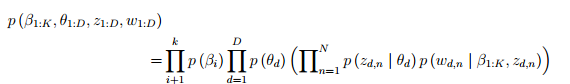
\includegraphics[width=1\textwidth]{ec1}
\caption{Ecuación de distribución conjunta \cite{DescubrimientoPatrones}}
\label{ecuacion1}
\end{figure}


Esta distribución especifica una serie de dependencias. La asignación del tópico zd,n
depende de la proporción del tópico $\theta$d por documento.
Las palabras observadas wd,n dependen de la asignación de tópico zd,n y de todos
los tópicos $(\beta)$1:K. Estas dependencias definen el modelo LDA.
Una vez definido el modelo que representa las relaciones entre los tópicos, los documentos
y las palabras existentes en un corpus, para que este sea de utilidad es necesario
calcular las distribuciones condicionales de la estructura de los tópicos, dada la colección
de documentos. Esta distribución es lo que se llama como posterior. La definición
posterior se desprende de la ecuación descrita en la figura \ref{ecuacion1} y se detalla en la figura \ref{ecuacion2}:\\

\begin{figure}[H]
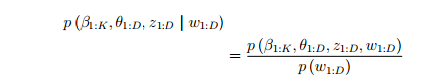
\includegraphics[width=1\textwidth]{ec2}
\caption{Ecuación de distribución conjunta alternativa \cite{DescubrimientoPatrones}}
\label{ecuacion2}
\end{figure}

El numerador es la distribución conjunta de todas las variables aleatorias, que pueden
ser fácilmente calculadas para cualquier conjunto de variables ocultas. El denominador
es la probabilidad marginal de las observaciones, que es la probabilidad de ver
el corpus observado bajo cualquier modelo de tópicos. En teoría, puede computarse
sumando la distribución conjunta de cualquier posible combinación de la estructura
de tópicos ocultos. Como para muchos problemas bayesianos, no se puede computar la
probabilidad posterior por el denominador, conocido como “evidencia”. Los algoritmos
de modelado de tópicos producen una aproximación de la ecuación \ref{ecuacion2} formando una
distribución alternativa a lo largo de la estructura latente de tópicos que se adapta para
acercarse a la real posterior.


\section{Word2vec}

Con el objetivo de la automatización del resumen de textos, se puede utilizar una
variedad de técnicas, como Hidden Markov Models , técnicas de grafos, y acercamientos
sobre distribución de probabilidades \cite{heuer2015semantic}. Propuesto por Sahlgren \cite{sahlgren2005methods} (hipótesis distributiva) las palabras con un significado similar
ocurren en similares contextos . Esto implica que el significado de las palabras se
puede inferir por su distribución contextual. Bruni y otros \cite{bruni2014multimodal} demuestran
que esta teoría tiene múltiples raíces teóricas estudios de lingüística , lexicografía
y filosofía. El objetivo de la semántica distributiva es encontrar una representación, por
ejemplo, un vector, que aproxime el significado de una palabra. La hipótesis distributiva
propone que los términos con propiedades de distribución similares tienen un significado
similar \cite{sahlgren2005methods}.
Uno de los desafíos de la semántica distributiva es computar vectores de palabras
que sean representaciones adecuadas de las palabras. Se utilizan varias arquitecturas
para computar tales vectores de palabras. Tradicionalmente, los vectores de palabras
se entrenan como parte de un lenguaje de modelado de redes neuronales. De acuerdo
con Mikolov, las redes neuronales artificiales pueden pensarse como una proyección
no lineal de los datos \cite{mikolov2013efficient}. Las redes neuronales artificiales (RNA)
son un sistema para el tratamiento de la información, cuya unidad de procesamiento
básica está inspirada en la neurona humana \cite{de1998aplicacion}. para ampliar más conceptos en redes neuronales ver 
\cite{rajasekaran2003neural}.


Word2vec fue desarrollado por Mikolov, Sutskever, Chen, Corrado y Dean en Google
y publicado en 2013 \cite{mikolov2013efficient}. Word2vec es una herramienta que implementa
dos formas de computar representaciones de palabras: continuous bag-of-words
(CBOW) y continuous skip-gram (CSG) .
Word2vec toma un corpus como entrada y produce vectores de palabras como resultado.
Primero construye un vocabulario desde los textos de entrenamiento y luego
aprende una representación vectorial de palabras, En \cite{goldberg2014word2vec} se ha demostrado que las representaciones vectoriales de palabras aprendidas
por los modelos word2vec tienen significados semánticos y conceptuales. El vector de palabras resultante puede
usarse como variables en aplicaciones de procesamiento de lenguaje natural y aprendizaje automático.
La ventaja que presenta Word2vec es su utilización de modelos de redes neuronales que
entienden el significado semántico de las palabras.
Las arquitecturas que se utilizaron previamente a CBOW y CSG fueron RNA alimentadas
hacia adelante (Feedforward Neural Net Language Model -NNLM) , y Redes
neuronales con conexiones recurrentes (Recurrent Neural Net Language Model -
RNNLM).
El modelo de lenguaje probabilístico de red neuronal feedforward (NNLM) se compone
de capas de entrada, capa de proyección, capa oculta y capas de salida. En la
capa de entrada, N palabras anteriores se codifican utilizando una de-codificación V ,
donde V es el tamaño del vocabulario. La capa de entrada es entonces proyectada a
una capa P proyección que tiene dimensión N * D, utilizando una matriz de proyección
compartida, donde D es la dimensionalidad de las palabras en el espacio. Como sólo N
entradas están activas en un momento dado, la composición de la capa de proyección
es una operación relativamente barata.
El modelo RNNLM no tiene una capa de proyección, sólo entrada, oculta y salida.
Lo que tiene especial este modelo es la matriz recurrente que conecta la capa oculta a
sí misma, usando conexiones demoradas en el tiempo. Esto permite al modelo recurrente
formar una memoria de corto plazo.
Continuous Bag-of-Words Model es similar a feedforward NNLM, donde la capa
oculta no lineal se remueve y la capa proyectada se comparte para todas las palabras,
por lo tanto, todas las palabras se proyectan en la misma posición (sus vectores se
promedian). Se llama a esta arquitectura modelo bag-of-words, porque el orden de las
palabras en la historia no influencia la proyección.
Continuous Skip-gram Model es similar a CBOW, pero en vez de predecir la palabra
basada en el contexto, trata de maximizar la clasificación de una palabra basada en
otra palabra en la misma oración. Se utiliza cada palabra como una entrada en un
clasificador log-lineal con una capa continua proyectada, y predice palabras con un
cierto rango antes y despúes de la actual palabra.
Aumentando el rango mejora la calidad de los vectores de palabras resultantes, pero
también incrementa la complejidad computacional. Desde que las palabras más distantes
están usualmente menos relacionadas con la palabra actual que aquellas cercanas a
ella, se les da menos peso a las palabras distantes muestreando menos de esas palabras
en los ejemplos de entrenamiento.
Para reducir el número de categorías y mejorar la eficiencia, la primera opción de
los investigadores fue el agrupamiento (clustering). La idea principal fue agrupar las
palabras similares en una clase y luego utilizarla para representar cada palabra. Los
vectores computados por Word2vec contienen información semántica. En word2vec la
mayor contribución es que se puede con exactitud calcular la similitud entre palabras
utilizando esos vectores \cite{yuan2014new}. 
Para ello, se pueden obtener las palabras similares calculando la similitud coseno
como medida de distancia. Se pueden agrupar estas palabras similares en la misma
clase computando la similitud coseno luego de definir el número de grupos. Luego de
obtener los grupos, se pueden contar las palabras que aparecen en él y sumar el número
como un valor de la dimensión correspondiente. El vector obtenido es la variable del
documento. Este vector integra la Información semántica de las palabras similares. Los
vectores de Word2vec se pueden utilizar como atributos para tareas de procesamiento
de lenguaje natural supervisadas, como clasificación de documentos, reconocimiento de
entidades nombradas y análisis de sentimiento.
Por ejemplo, en \cite{yuan2014new} se utilizaron dos conjuntos de datos. Luego del
pre-procesamiento , se armó un corpus.
Cada cinco palabras contiguas se tomó como una ventana, y se introdujo en
Word2vec. Se definió la dimensión del vector en 200. Se pudieron obtener n * 200
vectores despúes de entrenar la red neuronal, donde n es el número de palabras. Tomando
estos vectores, se utilizaron para calcular la similitud coseno cada dos palabras.
Luego, las palabras más similares se agruparon en un cluster. En el diseño de los experimentos,
se definió el número de clusters en 50. Luego se etiquetaron los clusters en cada
palabra y se computaron los features (atributos) de los documentos a través de estos
clusters. Se inicializaron los features en un vector de dimensión d * 50, donde d es el
número de documentos y cada columna representa un cluster. Si una palabra pertenece
al i-ésimo cluster aparece en el documento, el correspondiente feature sumaría +1 en
la i-ésimo dimensión. Con esta metodología, se obtuvieron todos los vectores de features.
Se dividieron los datos en entrenamiento y testing, y se entrenó  un clasificador SVM
(Support Vector Machine, ver en \cite{tong2001support}. Se compararon los resultados
de esta metodología versus LDA y TF-IDF . En ambos conjuntos de
datos, el resultado utilizando word2vec fue superior al resto.

\textbf{Modelo continuo de bolsa de palabras (Continuous Bag-of-Word Model)}



Partiendo del modelo básico de \cite{mikolov2013efficient},
 \cite{goldberg2014word2vec} supone que solo se considera una palabra por contexto, lo que significa que el modelo predecirá una palabra objetivo dada una palabra de contexto, que
es como un modelo de bigrama. La idea es tratar las palabras alrededor de una palabra central como su contexto. E.g., {“El”, “gato”, “se”, “sobre”, “el”, “sillón”} viene a ser el contexto de
la palabra “sentó” \cite{cardellinoproyecto}.

La Figura \ref{redcbow} muestra el modelo de red bajo la definición de contexto simplificada.

\begin{figure}[H]
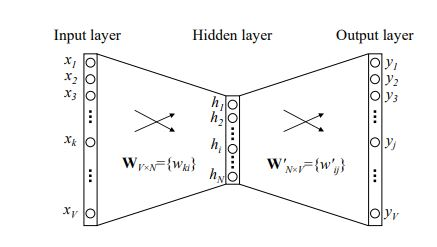
\includegraphics[width=1\textwidth]{redcbow}
\caption{Un modelo CBOW simple con solo una palabra en el contexto \cite{goldberg2014word2vec}}
\label{redcbow}
\end{figure}



 En la configuración, el tamaño del vocabulario es V, y el tamaño de la capa oculta es N. Las unidades de las capas adyacentes están completamente conectadas. La entrada es un vector ''one-hot encoding'', lo que significa que para un
palabra de contexto de entrada, solo una de V unidades, {x1, · · ·, xV}, será 1, y todas las demás unidades serán 0.
Según \cite{cardellinoproyecto} se toma como punto inicial el vocabulario V = w ^{(1)}$, w^{(2)}$, . . . , w^{(m)}$ (|V | = m). A cada palabra w^{(i)}$ se la representa con un vector one-hot x^{(i)}$ \in {R^{m}$}. Para definir los parámetros a actualizar, creamos dos matrices W^{(1)}$  \in R^{m \times n}$ y W^{(2)}$  \in R^{n \times m}$. Donde n es la dimensión final que queremos para los vectores aprendidos  .

Continuando la propuesta de \cite{cardellinoproyecto} La matriz W^{(1)}$ está formada por m filas u^{(i)}$ \in R^{n}$ , estas representan el vector codificado de entrada de la palabra w^{(i)}$ . A su vez, la matriz de salida W^{(2)}$ se conforma de m columnas v^{(j)}$ \in R^{n}$ , que representan el vector codificado de salida de la palabra w^{(j)}$ . Es decir, por cada palabra del vocabulario, se aprenden dos vectores de palabras.

El modelo de CBOW consta de los siguientes pasos:

\begin{itemize}
	\item Se busca obtener la palabra central w^{(i)}$ dado el contexto. (w^{(i - C)}$, . . . , w^{(i -1)}$, w^{(i+1)}$, . . . , w^{(i+C)}$).
	\item Se genera los vectores one-hot para cada una de las palabras del contexto (x^{(i - C)}$ , . . . , x^{(i - 1)}$, x^{(i+1)}$, . . . , x^{(i+C)}$ ).
	\item Obtenemos los vectores codificados de entrada por cada vector one-hot (u^{(i - C)}$ = x^ {(i - C)}$^{T}$ W^{(1)}$, . . . , u^{( i - 1)}$ = x^{ (i -1)}$^{T}$ W^{(1)}$, u^{(i+1)}$ = x^{ (i+1)}$^{T}$ W^{(1)}$, . . . , u^{(i+C)}$ = x^{(i+C)}$^{T}$ W^{(1)}$).
	\item Se busca la media de los vectores para obtener un vector\\  h =(u^{(i - C)}$+u^{(i - C+1)}$+···+u^{ (i+C)}$ ) /(2C) .
	\item Y lo transformamos en un vector de probabilidades mediante y^{'}$ = softmax(z).
	\item Queremos que las probabilidades  y^{'}$^{(i)}$ , sean iguales a las probabilidades correctas, y^{(i)}$, i.e,el vector one-hot de la palabra w^{(i)}$.
\end{itemize}

Una vez se sabe la funcionalidad del modelo en caso de tener los valores correctos para W^{(1)}$ y W^{(2)}$, se pregunta cómo aprender dichas matrices. Si se observa, se entiende que las matrices forman una red neuronal que se entrena mediante retro-propagación y cuya arquitectura se muestra en la Figura  \ref{redcbow}. 


\textbf{Modelo de Skip-Gram}

SkipGram es el otro modelo propuesto por Mikolov \cite{mikolov2013efficient}. Difiere de CBOW ya que busca, dada una palabra central llamada contexto (e.g., “sentó”), predecir las palabras que conforman su alrededor (e.g, “El”, “gato”, “se”, “sobre”, “el”, “sillón”).
 Similar CBOW, solo cambian los papeles de los vectores codificados de entrada (que pasa a ser uno solo) y los vectores codificados de salida (que pasan a ser varios)\cite{goldberg2014word2vec}.
Las matrices siguen siendo las mismas. El modelo skip-gram, trabaja de la siguiente manera:

\begin{itemize}
\item Buscamos obtener las palabras (w^{ (i - C)}$ , . . . , w^{(i - 1)}$, w^{(i+1)}$, . . . , w^{(i+C)}$ ), dada la palabra central w ^{(i)}$ .
\item Generar el vector one-hot para la palabra de entrada x^{(i)}$ .
\item Obtener el vector codificado de entrada u^{(i)}$ = x^{( i)^{T}$}$W^{(1)}$ .
\item Como es un solo vector de entrada, no hay necesidad de obtener la media. Definimos h = u^{(i)}$ .
\item Se genera 2C vectores de puntaje (z^{(i - C)}$ , . . . , z^{(i - 1)}$, z^{(i+1)}$, . . . , z^{(i+C)}$ ) con z^{(j)}$ = h^{(T)}$W^{(2)}$
\item Se Transforma cada vector de puntaje en un vector de probabilidades,  y^{'}$^{(j)}$ = softmax(z^{(j)}$).
\item Se quiere que los vectores de probabilidad generados  (  y^{'}$^{(i - C)}$ , . . . ,   y^{'}$^{(i - 1)}$ ,  y^{'}$^{ (i+1)}$ , . . . ,   y^{'}$^{(i+C)}$ ), sean iguales a las probabilidades verdaderas, (y^{(i - C)}$ , . . . , y^{(i - 1)}$, y^{(i+1)}$, . . . , y^{(i+C)}$ ), i.e. de los vectores one-hot por cada palabra de salida.
\end{itemize}

Similar al modelo CBOW, se calcula los valores de las matrices W^{(1)}$ y W^{(2)}$ . Nuevamente las matrices forman una red neuronal que se entrenara mediante retro-propagación y cuya topología se muestra en la Figura \ref{redskg}.

\begin{figure}[H]
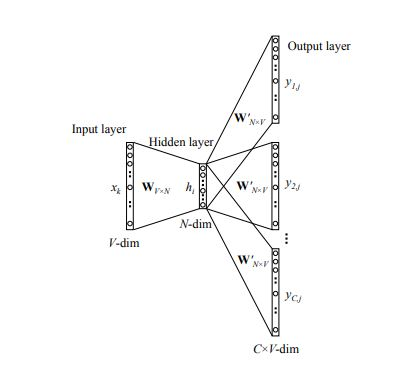
\includegraphics[width=1\textwidth]{redskg}
\caption{Topología del modelo Skip-Gram \cite{mikolov2013efficient}}
\label{redskg}
\end{figure}

\section {Document Embeddings con Doc2Vec}

Doc2Vec es una técnica para representar documentos como vectores de longitud fija y baja dimensionaldad (conocidos también como document embeddings).
Fue creado por Mikolov y Le \cite{le2014distributed} en 2014 en su paper “Distributed Representations of Sentences and Documents”. Mikolov, es también uno de los autores del modelo antes mencionado Word2Vec \cite{mikolov2013efficient}.


En las pruebas realizadas en \cite{capello2018sistema} se ve como Doc2vec supera a otros métodos,
Doc2vec es una extensión del modelo Word2vec.  

La representación vectorial de Doc2vec se crea usando alguno de los dos algoritmos o modelos incorporados: Continuous Bagof-Words (CBOW) y Skip-Gram.

Doc2Vec, tiene dos algoritmos para obtener los embeddings: PV-DM (Paragraph Vector - Distributed Memory) y PV-DBOW (Paragraph Vector - Distributed Bag of Words). Cada uno surge de la extensión de los algoritmos wor2vec anteriormente descritos, respectivamente.

\textbf{PV-DM}

El modelo PV-DM está basado en el modelo Word2vec CBOW, la cual consiste en una red neuronal con tres capas: una de entrada (input), una oculta (o hidden layer) y una de salida (ouptut); con ella se aprenden representaciones de palabras dado un determinado contexto.

El método a Doc2Vec (PV-DM, Figura \ref{pvdm}) extiende de CBOW, se agregan nodos de entrada adicionales (contexto adicional), un nodo por cada documento identificados inicialmente por los ids: 0, 1, …, |Corpus|-1. Por lo tanto, se extiende aún más la capa de entrada.

\begin{figure}[H]
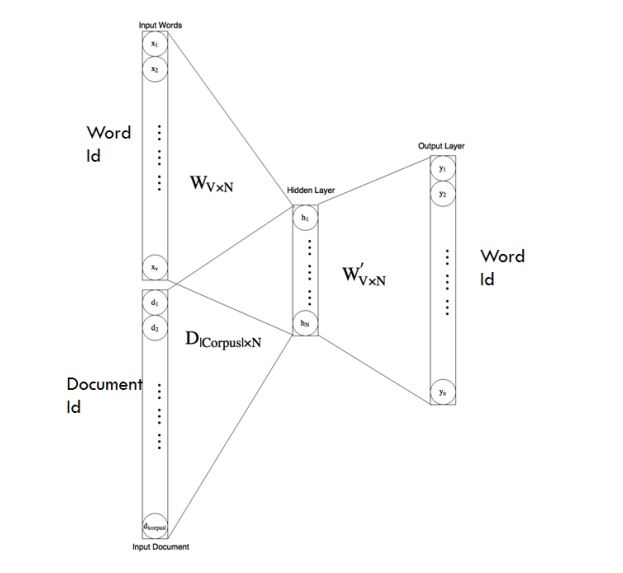
\includegraphics[width=1\textwidth]{pvdm}
\caption{Red neuronal ilustrativa en PV-DM \cite{capello2018sistema}}
\label{pvdm}
\end{figure}


Después se ejecuta el algoritmo de retro-propagación de la misma forma descrita en CBOW, con el id correspondiente al id del documento con el cual se está entrenando, para el cual pertenece la oración seleccionada.  Una vez finalizado el proceso de entrenar contextos de palabras junto con el id del documento, se terminan obteniendo en la matriz D document embeddings y en la matriz W word embeddings. Mediante medidas de similitud, como la del coseno, se hallan los vectores más semejantes a uno fijado, tanto en W, como en D; dependiendo del interés.

\textbf{PV-DBOW}

El modelo de Distributed Bag of Words (DBOW) es la contraparte al modelo PV-DM. El modelo DBOW no tiene en cuenta las palabras de contexto en la entrada, pero obliga al modelo a predecir palabras muestreadas aleatoriamente del documento (dentro de la “ventata”), en la salida. En el ejemplo que se aprecia en la
Figura  \ref{doc2veceje} el modelo aprende mediante  la predicción de 4 palabras muestreadas. Por tanto, para aprender el vector de documento, se muestrean 4 palabras de (the, cat, sat, on, the, mat), repitiendo este proceso un gran número de veces análogamente al anterior proceso, para varias muestras en el documento.

\begin{figure}[H]
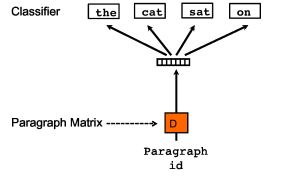
\includegraphics[width=1\textwidth]{doc2veceje}
\caption{ PV-DBOW simplificado \cite{le2014distributed}}
\label{doc2veceje}
\end{figure}




%https://nlp.cic.ipn.mx/Publications/2010/Generacion%20de%20grafos%20conceptuales.pdf

%http://www.scielo.org.mx/scielo.php?pid=S0187-358X2017000100103&script=sci_arttext&tlng=en

\section{K-means (K-M)}

En \cite{manning2010introduction} afirman que el objetivo del algoritmo k-media
es minimizar el error cuadrático medio de la distancia Euclidiana de los documentos con respecto al centroide del grupo 
al cual hacen parte. El centro de un agrupamiento es definido como la media o centroide de los documentos que están en un agrupamiento.

Según \cite{witten2016data} a La métrica para ver si un centroide representa bien a sus miembros del grupo,
es la suma residual cuadrática (SRC), 
que es la sumatoria de la distancia cuadrática de todos los vectores con relación al centroide.
El SRC es la función objetiva del k-media y el objetivo es minimizarla,el algoritmo de k-media no garantiza que 
será alcanzado el mínimo global al utilizar la función objetiva,por ejemplo, si la muestra posee 
muchos valores atípicos no se ajustará bien a ninguno de los agrupamientos.

Otro problema del k-media es que debido a la selección aleatoria inicial de los centroides, 
los agrupamientos resultantes pueden variar mucho en calidad y finalmente el método k-media no sirve
para descubrir agrupamientos con formas no convexas o agrupamientos con diferentes tamaños \cite{wang2011new}.



\section{Antecedentes}

Las organizaciones mayormente disponen de información en documentos de texto no estructurado ,
se encuentran tipificados de esa manera ya que la información contenida en el documento no tiene ningún orden de estructura, ésta
información tiene mayor riesgo de no ser encontrada por los buscadores, pues no contiene parámetros establecidos que proporcionen
la información que se está buscando y sea presentada al usuario, por esta razón la minería de texto adquiere un rol importante
ya que es el proceso de extraer información interesante y conocimiento no trivial de textos no estructurados incluyendo tecnologías 
para extracción de información, seguimiento de temas, generación automática de resúmenes de textos, categorización,
agrupamiento , relaciones entre conceptos , visualización y respuesta automática de preguntas .  

\cite{troyano2003identificacion} describe los principales enfoques de extracción y reconocimiento de NER (entidades con nombre ) , 
el NER desempeña un papel muy importante en diversos problemas relacionados a la búsqueda automática y la categorización de textos.
 
En \cite{figuerola2004algunas} se propone un nuevo método para la caracterización de documentos que sin importar el idioma en el que el 
documento esté escrito, permite extraer el conjunto de palabras clave más adecuado. Su funcionamiento se basa en una Red Neuronal, que
luego de ser entrenada es capaz de decidir para cada término del documento si se trata de una palabra clave o no. El ingreso del documento a la Red Neuronal implicó la definición de una representación numérica adecuada que permite medir la participación de un término dentro del documento.

Utilizando  las técnicas de minería de texto se pretende obtener una serie de conjuntos de datos estructurados, 
para poder aplicar algoritmos de aprendizaje automático como se lo propone en \cite{llorens1998caracteristicas}, 
\cite{santana2014aplicacion}, \cite{barrera2016mineria} y \cite{rodriguez2018metodos}  logrando una categorización
y clasificación de documentos adecuada, \cite{ropero2014metodo}  propone un método que relaciona e integra técnicas de procesamiento de lenguaje natural,
agrupamiento (clustering) y modelos de Markov como una solución de bajo costo, dependiente del dominio, para la evaluación automática 
de la organización en textos argumentativos. 

Otra propuesta de utilización de minería de texto es la de Grobelnik, Mladenic  and Jermol  \cite{grobelnik2002exploiting}, en la cual se pretende potenciar una aplicación de construcción de ontologías/taxonomía a
partir de un conjunto de documentos planos, realizar búsquedas en la base de documentos y tratar problemas específicos del lenguaje,
por su parte \cite{cobo2006tecnicas},\cite{neto2000document} proponen sistemas  para resumir textos, agrupar documentos e interpretar el conocimiento de los grupos obtenidos para una  fácil compresión  por parte  del usuario.

Arco et al.\cite{arco2006agrupamiento} estudia el impacto de la representación del texto en el ámbito de la clasificación no supervisada (CNS) de documentos.
Tomando como referencia una representación basada en un modelo de espacio vectorial de términos, se analizan diferentes
técnicas de representación de los datos sobre espacios de menor dimensionalidad (obtenidas mediante técnicas de extracción de
términos como el Análisis de Semántica Latente, la Factorización en Matrices No Negativas y el Análisis en Componentes Independientes)
para mejorar la CNS de un corpus de documentos.

En \cite{MONTESYGOMEZ2005} y \cite{munozutilizacion} emplean minería de texto para la semejanza entre estructuras semánticas
usando grafos conceptuales como representación del contenido de los textos, y obtiene algunos patrones descriptivos de los documentos aplicando varios tipos de operaciones sobre estos grafos.


%\section{Hierarchical Agglomerative Clustering (HAC)}

%El agrupamiento jerárquico aglomerativo (HAC) es un método de aprendizaje no supervisado. El HAC es un algoritmo de agrupamiento 
%jerárquico de abajo para arriba que considera inicialmente cada documento como un agrupamiento individual y luego sucesivamente
%va fusionando los agrupamientos en pares, teniendo en cuenta la similitud entre ellos, hasta que todos los agrupamientos 
%se aglomeren en un único agrupamiento que contiene todos los documentos presentados al algoritmo \cite{suh2010extraction}.

%Para el cálculo de similitud se utilizan diferentes técnicas de medidas de similitud como el agrupamiento de link simple, 
%el agrupamiento de link completo, agrupamiento aglomerativo de media del grupo y agrupamiento por centroide \cite{witten2016data}.

%Para la visualización de los HAC es utilizado generalmente un dendrograma, donde cada unión (et al aglomeración) 
%es representada por una línea horizontal entre los dos agrupamientos y el valor de la similitud entre esos 
%dos agrupamientos esta especificado en el eje Y. El HAC tiene la suposición fundamental que es la
%monotonicidad en las operaciones de aglomeración (merge operation).







\chapter{Materiales y Métodos}

Se utilizó el repositorio de datos de los trabajos de grado de la biblioteca Alberto Quijano Guerrero de la universidad de Nariño. 

En este capítulo se describen los procesos de construcción, limpieza y transformación
del corpus de documentos de los trabajos de grado. Luego se detallan los experimentos
realizados; con el objetivo de descubrir relaciones conceptuales en el corpus de trabajos
de grado de la Universidad de Nariño utilizando la metodología CRISP-DM.



\section{Comprensión del problema}

En esta fase, se realizaron las actividades que permitieron profundizar y apropiar de una manera completa el problema objeto de estudio, los objetivos y los requisitos de esta investigación,
 que posibilitaron la recolección de los datos correctos para interpretar adecuadamente los resultados. En esta fase, descubrir las relaciones conceptuales del repositorio de documentos no estructurados de trabajos de grado de la universidad de Nariño,
 se convirtió en un problema a resolver con minería de textos.  Como resultado de la fase de compresión se construyó un marco teórico de diferentes técnicas de minería  de textos para abordar el problema; contemplado en el capítulo anterior.

\section {Comprensión de los datos}

En esta fase, se identificó, recopiló y familiarizó con el corpus de trabajos de grado, disponible en el repositorio de la biblioteca Alberto Quijano Guerrero de la universidad de Nariño.
Se construyó un repositorio inicial donde se integraron todos los trabajos de grado de los diferentes programas de la universidad de Nariño. Dando como resultado un repositorio compuesto por 8.076 documentos no estructurados, el cual sirvió de base para las subsiguientes fases. 

\section{Preparación de los datos}
En la fase de preparación se realizó el pre procesamiento del corpus primero que todo se descartó de los textos la sección de agradecimientos,
 utilizando expresiones regulares; se obtuvo las secciones de resumen, introducción, marco teórico, metodología, resultados y conclusiones.
 Después de eliminar la sección de agradecimientos se eliminaron las palabras muertas de la colección usando la librería Spacy de Python,
 seguidamente se lematizaron las palabras del corpus, ejemplo desarrollo por desarrollar.  Obteniendo como resultado un corpus limpio y listo para el desarrollo del trabajo. La figura  \ref{fig:proceso1} detalla el proceso de pre procesamiento del corpus.

\begin{figure}[H]
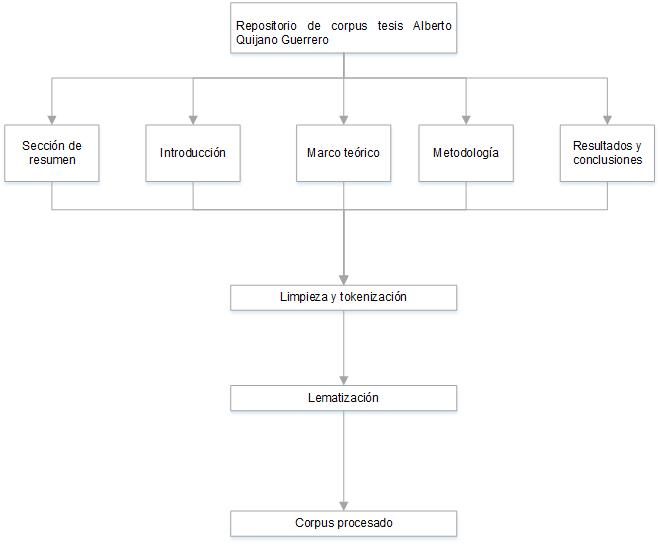
\includegraphics[width=1\textwidth]{proceso1}
\caption{Flujo de trabajo para el armado del corpus}
\label{fig:proceso1}
\end{figure}



\section{Modelado}

Una vez organizado el corpus se implementaron diferentes técnicas de minería de texto; para obtener diferentes conjuntos de datos estructurados .
Para estructurar documentos se usaron tres técnicas diferentes, las dos primeras proveniente de la librería Sklearn; CountVectorizer (Bow) y TfidfVectorizer (TF-IDF); la tercera técnica utilizada fue Doc2vec proveniente de la librería Gensim. 


\textbf{Modelos Bow y TF-IDF}

A continuación, se describen los parámetros establecidos para la generación de los modelos Bow y TF-IDF de la librería Sklearn; los cuales comparten los mismos parámetros.
\begin{itemize}
	\item Max\_df: Al construir el vocabulario, ignora los términos que tienen una frecuencia de documento estrictamente más alta que el umbral dado (palabras vacías específicas del corpus). Este parámetro toma un rango devalores [0, 1]. Para nuestro caso se usó en 0.7, ignorando los términos que estén presentes como mínimo en el 70\% de los documentos. 
	\item Min\_df: Al construir el vocabulario, ignora los términos que tienen una frecuencia de documento estrictamente más baja que el umbral dado. Este valor también se llama corte en la literatura. Toma valores en el rango de [0, 1], el parámetro representa una proporción de documentos, recuentos enteros absolutos. Paranuestro caso se elige 0.01;
		 eliminando términos que solo aparecen en el 1\% delos documentos.
	\item Ngram\_range: Límite inferior y superior del rango de valores n para los diferentes n-gramas que se van a extraer. Por ejemplo, un ngram\_range de (1, 1) utilizara solo unigramas, (1, 2) utilizará unigramas y bigramas, y (2, 2) utilizara solo bigramas. Para nuestro caso se usó (1,2) generando unigramas y bigramas.
	\item Max\_features: Máximo número de variables a generar. Para nuestro caso se generaron  2 modelos con 10.000 y 20.000 variables.

\end{itemize}


\textbf{Modelos Doc2vec}

A continuación, se describen los parámetros establecidos para el entrenamiento de los modelos Doc2vec PV-DBOW y PV-DM de la librería Gensim; los cuales comparten los mismos parámetros.

\begin{itemize}
  \item Dm: Esto define el algoritmo de entrenamiento. Por defecto  (dm = 1), se utiliza memoria distribuida (PV-DM). De lo contrario, una bolsa distribuida de palabras (PV-DBOW) es empleado, para nuestro caso se usó los  dos métodos propuestos  por el modelo doc2vec dm=0 y dm=1 
  \item Size: Tamaño del vector de salida para la representación un documento, se eligió 20.
  \item Window: Esta es la distancia máxima entre la palabra predicha y el contexto de palabras utilizadas para la predicción dentro de un documento, se eligió un valor de 10.
  \item Alpha: Esta es la tasa de aprendizaje inicial (caerá linealmente a min\_alpha a medida que el entrenamiento progresa), se eligió 0.025.
  \item Min\_count: Ignora todas las palabras con una frecuencia total inferior a esta, se eligió 50 para limitar el tamaño del vocabulario a palabras significativas. Se ignora cualquier palabra que aparezca menos de 50 veces.
\end{itemize}

Para iniciar el análisis, se verifica si existe tendencia al agrupamiento en cada uno de los conjuntos de datos estructurados por los modelos generados anteriormente. Utilizamos el estadístico de Hopkins para establecerlo, recurrimos al paquete RANN de R. Seleccionamos 1000 puntos al azar de los datos de muestra y luego se los compara con 1000 puntos creados al azar. Luego se calcula la distancia al vecino más cercano de ambas muestras y finalmente se establece el estadístico para cada conjunto de datos.  La figura  \ref{fig:proceso2} detalla el proceso.

\begin{figure}[H]
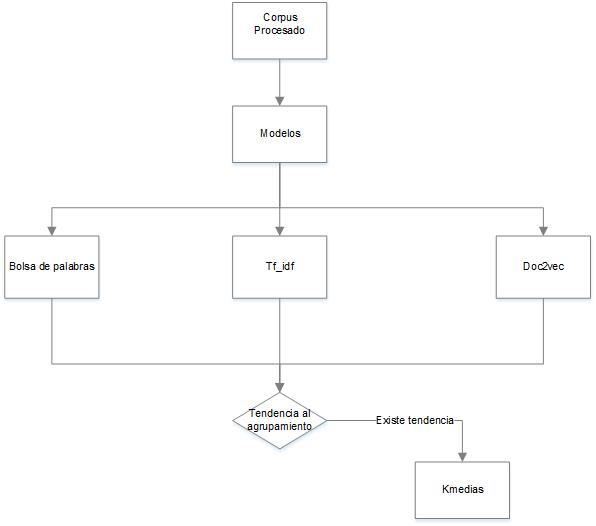
\includegraphics[width=1\textwidth]{proceso2}
\caption{Flujo de trabajo para la generación de un conjunto de datos estructurado }
\label{fig:proceso2}
\end{figure}

%
%
%La tabla \ref{tab:ProgramasDM} muestra el estadístico de Hopkins para cada conjunto de datos generado. 
%
%
%\begin{table}[H]\centering
%	\caption{Descripción de la tendencia al agrupamiento en los conjuntos de datos.}\label{tab:ProgramasDM}
%	\begin{tabularx}{\textwidth}{XXXm{6.0cm}}\toprule
%
%Modelo &  \multicolumn{1}{c}{Estadístico Hopkins} & \multicolumn{1}{c}{Descripción} \\ 
%Bow & 0.61 & Modelo Bow generando un conjunto de datos de 10.000 filas * 20.000 
%columnas usando unigramas y bigramas.
%Este método descarta términos que aparezcan en más del 70\% de documentos.  \\ 
%Bow &  0.58 & Modelo Bow generando un conjunto de datos de 10.000 filas * 10.000 
%columnas usando unigramas y bigramas.
%Este método descarta términos que aparezcan en más del 70\% de documentos.   \\ 
%Tf-idf & 0.54 & Modelo Tf-id generando un conjunto de datos de 10.000 filas * 20.000 
%columnas usando unigramas y bigramas.
%Este método descarta términos que aparezcan en más del 70\% de documentos.  \\ 
%Tf-idf &  0.52 & Modelo Tf-id generando un conjunto de datos de 10.000 filas * 10.000 
%columnas usando unigramas y bigramas.
%Este método descarta términos que aparezcan en más del 70\% de documentos.   \\ 
%Doc2vec & 0.38 & Este método representa un documento mediante 
%un vector de tamaño 20
%usando el algoritmo bolsa de palabras distribuida  (PV-DBOW)   \\ 
%Doc2vec & 0.42  & Este método representa un documento mediante
%un vector de tamaño 20
%usando el algoritmo memoria distribuida (PV-DM) \\  \bottomrule
%	\end{tabularx}
%
%\end{table}
%
%Con un umbral establecido en 0.5 podemos confirmar que existe tendencia al agrupamiento en los conjuntos de datos generados por los modelos Doc2vec bolsa de palabras distribuida (PV-DBOW) y Doc2vec memoria distribuida (PV-DM).
%%Los resultados muestran una mejor tendencia al agrupamiento en los modelos Doc2vec,
%Los modelos Doc2vec  logran captar relaciones conceptuales mediante el contexto que representa cada documento, usando esta representación se podrá medir qué tan relacionado está un documento con respecto a los demás.	

\textbf{Agrupación}

La agrupación es un ejercicio popular de aprendizaje automático, y las técnicas utilizadas en las tareas de clustering clásicas pueden utilizarse para texto una vez estructurado, con la idea de formar grupos de trabajos de grado de acuerdo a su dominio de conocimiento, para posteriormente entrenar el modelo word2vec en cada grupo o área específica encontrada. Para determinar la cantidad de grupos óptimos (K) se corrió el algoritmo kmedias para diferentes K, variando desde 20 hasta 44. Se calculó la suma de errores al cuadrado (SSE) y el coeficiente de Silhouette para cada valor de K. SSE mide la distancia de los puntos al centroide por lo cual esperamos que SSE sea lo más bajo posible. El coeficiente de Silhouette es útil para analizar la cohesión y la separación del agrupamiento, valores cercanos a 1 indican que el agrupamiento es bueno, valores alrededor de cero o hasta negativos indican que el k no es el óptimo o la tendencia al agrupamiento no es tan buena. Para la tarea de agrupación se usó la librería sklearn de Python y el algoritmo kmeans en los conjuntos de datos estructurados con tendencia al agrupamiento. 


%\begin{figure}[H]
%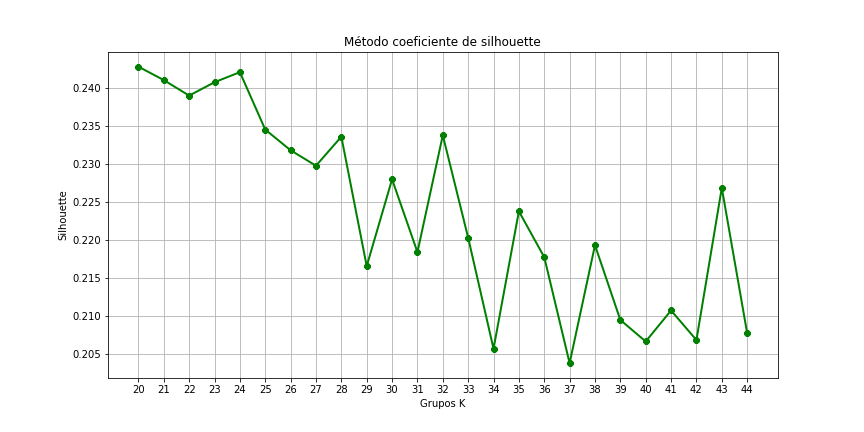
\includegraphics[width=1\textwidth]{Silhouette}
%\caption{Método coeficiente de Silhouette algoritmo Kmedias }
%\label{fig:proceso3}
%\end{figure}
%
%\begin{figure}[H]
%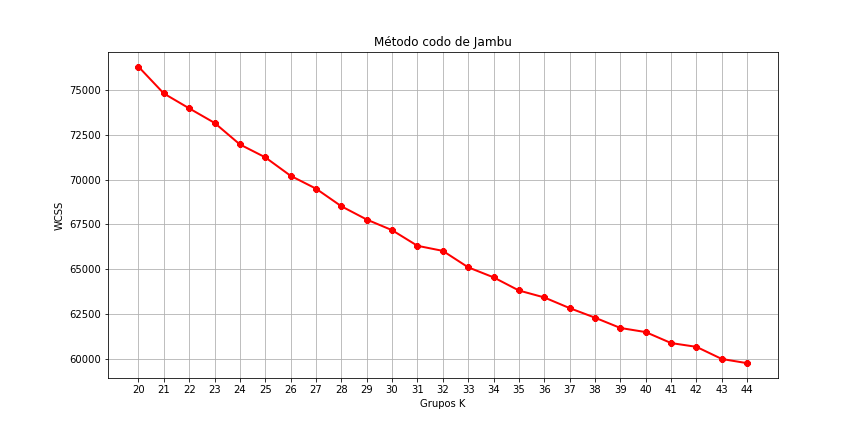
\includegraphics[width=1\textwidth]{WCSS}
%\caption{Método de codo de Jambu algoritmo Kmedias}
%\label{fig:proceso4}
%\end{figure}
%
%En la figura  \ref{fig:proceso3} se visualiza el método de coeficiente de Silhouette; el cual sugiere que el número adecuado de grupos es de 24, en la figura  \ref{fig:proceso4} se visualiza el método del codo de Jambu; 
%para el cual miramos que a medida que k se incrementa la distancia de los puntos al centroide va disminuyendo. Para la selección del K óptimo  se contrasto los dos métodos y se eligió el k en 32; ya que miramos que su coeficiente de Silhouette está entre los más altos y a la vez la distancia de los puntos al centroide es baja. 

\textbf{Modelo Word2vec}

Por cada grupo encontrado se entrenó el modelo Word2vec, con el fin de encontrar relaciones conceptuales entre los términos de dominio presentes en los documentos. 
Para este proceso se configuró un cluster con Apache Spark con el fin de paralelizar el entrenamiento y acelerar el tiempo de procesamiento, se utilizó la librería Pyspark para la programación en paralelo y la librería Gensim para el entrenamiento del modelo Word2vec y como entrada el corpus de lemas clasificado por su respectivo grupo encontrado.


Se utilizaron los siguientes parámetros para el entrenamiento:

\begin{itemize}
  \item	SG: Define el algoritmo de entrenamiento. Por defecto (sg = 0), se utiliza continuous bag of words (CBOW). De lo contrario (sg = 1), se emplea skip-gram, Skip-gram es más lento, pero produce mejores resultados por lo cual se eligió (sg=1).
  \item	Window: esta es la distancia máxima entre la palabra actual y la predicha dentro de una oración, se eligió 10.
  \item	Size: Este es el tamaño de los vectores que representan a un término, Valores razonables son entre 10 y cientos, se eligió 200.
  \item	Alpha: Esta es la tasa de aprendizaje inicial (caerá linealmente a min\_alpha a medida que el entrenamiento progresa), se eligió 0.03.
  \item	Min\_count: Ignora todas las palabras con una frecuencia total inferior a esta, se eligió 50 para limitar el tamaño del vocabulario a palabras significativas. Se ignora cualquier palabra que aparezca menos de 50 veces.
  \item	Workers: Número de núcleos a utilizar para el procesamiento del trabajo. Para el caso se utilizó todos los núcleos disponibles de la máquina.
  \item	hs: Si es 1, softmax jerárquico se utilizará para el entrenamiento del modelo. Si se establece en 0 (predeterminado), y negativo es distinto de cero, se utilizará un muestreo negativo, se eligió 1 softmax jerárquico.
  \item	Iter: Este es el número de iteraciones (épocas) sobre el corpus. El valor establecido para el caso fue 6000.
\end{itemize}

\textbf{Clasificación}

Para clasificar futuros trabajos que se ingresen a Maskana se entrenaron varios modelos de aprendizaje supervisado, donde la clase a aprender es el grupo o categoría encontrada por el algoritmo k-medias y las variables predictoras son los vectores generados por el algoritmo Doc2vec.
La figura \ref{fig:procesocalsificacion} detalle el proceso de entrenamiento de los diferentes modelos de aprendizaje supervisado.


\begin{figure}[H]
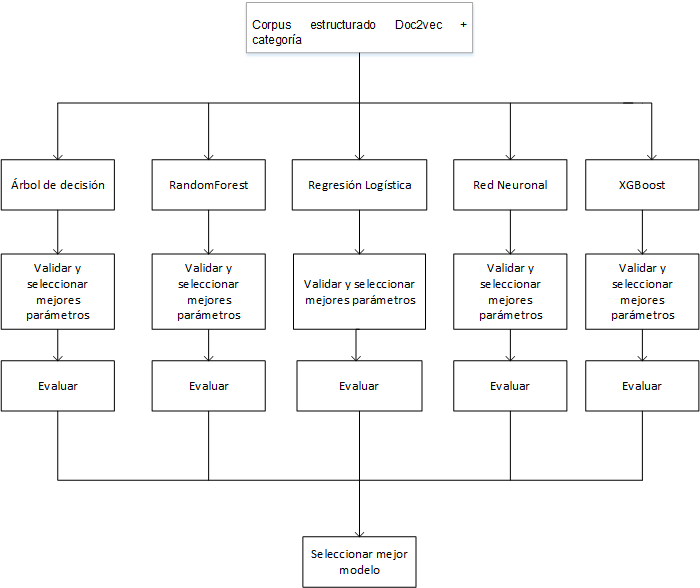
\includegraphics[width=0.9\textwidth]{procesocalsificacion}
\caption{Flujo de trabajo para el entrenamiento de modelos de aprendizaje supervisado.}
\label{fig:procesocalsificacion}
\end{figure}

Para el entrenamiento de estos modelos se usó el módulo mlib de la librería pyspark. Para cada modelo de clasificación, se implementó una grilla  de búsqueda para iterar sobre los  hiperparámetros  mediante el método de validación cruzada y la métrica de accuracy (exactitud).

A continuación se detalla la selección de los  parámetros de cada modelo:

\textbf{Árboles de decisión}

\begin{itemize}
	\item MaxDepth: Profundidad máxima del árbol. Se itero este parámetro con valores de  [3, 5, 10, 15, 20], el mejor resultado se lo obtuvo con maxDepth=5.
	\item MinInstancesPerNode: Número mínimo de instancias que debe  recibir un nodo para dividirse. Se itero este parámetro con valores de  [5, 10, 15, 20, 50], los mejores resultados se obtuvieron con minInstancesPerNode=10. 
	\item Impurity: Medida de impureza utilizada para elegir entre posibles divisiones. Se itero sobre los dos posibles valores de este parámetro ['entropy','gini'], se obtuvieron mejores resultados con impurity= 'entropy'.
\end{itemize}

\textbf{RandomForest}

\begin{itemize}
	\item NumTrees: Número de árboles en el bosque aleatorio .Se itero con valores de [100,500,1000], los mejores resultados se obtuvieron con numTrees=500.
	\item MaxDepth:Profundidad máxima de los árboles del bosque aleatorio. Se itero con valores de  [3, 5, 10, 15, 20], los mejores resultados se obtuvieron con maxDepth=10.
	\item MinInstancesPerNode: Número mínimo de instancias que debe  recibir un nodo para dividirse. Se itero este parámetro con valores de  [5, 10, 15, 20,50], los mejores resultados se obtuvieron con un valor de minInstancesPerNode=5. 
	\item Impurity: Medida de impureza utilizada para elegir entre posibles divisiones. Se itero sobre los dos posibles valores de este parámetro ['entropy','gini'], se obtuvieron mejores resultados con impurity= 'gini'.
	\item MinInfoGain: Para que un nodo se divida aún más, la ganancia de información que genera la división debe superar el valor mínimo establecido.Se itero con valores de   [0.0, 0.25, 0.5, 0.75],  se obtuvieron mejores resultados con minInfoGain=0.25
\end{itemize}

\textbf{Regresión Logística}
\begin{itemize}
	\item Max\_iter: Número máximo de iteraciones que se toman para que los solucionadores converjan. Se itero este parámetros con [10.000, 20.000], se obtuvo mejores resultados con  max\_iter=10.000.
	\item Penalty: Se utiliza para especificar la norma utilizada en la penalización. Se itero con ['l1', 'l2'], obteniendo mejores resultados con penalty= 'l1'.
	\item Class\_weight: Pesos asociados a las clases del entrenamiento. Si no se da, se supone que todas las clases tienen un peso uno. El modo 'balanceado' usa los valores de la variable Y, para ajustar automáticamente los pesos inversamente proporcionales a las frecuencias de clase en los datos de entrada como n\_samples / (n\_classes * np.bincount (Y)). Se itero este parámetros con [none,'balanced']; alcanzando un mejor resultado con  class\_weight='balanced'
\end{itemize}

\textbf{Red Neuronal}



\begin{itemize}
	\item La capa de entrada consta de 20 neuronas para las variables de entrada generadas por el modelo Doc2vec.
	\item En la capa de salida se configuró 32 neuronas, una  por cada categoría encontrada.
	\item En las capas de entrada y capas ocultas se usó la función de activación logsig y en la capa de salida la función softmax.
	\item Para el entrenamiento de la red neuronal se probó y validó diferentes arquitecturas  [20, 1 , 32], [20, 5 , 32] , [20, 10, 32], [20, 10, 10, 32] y [20, 15, 15, 32].
	\item La arquitectura que mejor resultados obtuvo fue [20, 10, 10, 32]; 20 neuronas de entrada, 2 capas ocultas con 10 neuronas interconectadas y 32 neuronas en la capa de salida. 

\end{itemize}

\textbf{XGBoost}

\begin{itemize}
	\item N\_estimators: Número de árboles con aumento de gradiente, Se definió este parámetro en 500.
	\item Learning\_rate: El parámetro learning\_rate se puede configurar para controlar la ponderación de los árboles nuevos agregados al modelo y así evitar el sobreajuste. Se itero con valores de [0.3, 0.1,  0.01], Se obtuvo  mejores resultados con learning\_rate= 0.3.
	\item Max\_depth: Profundidad máxima de un árbol. Incrementar este valor hará que el modelo sea más complejo y más probable que se sobreajuste.se itero este parámetro con [3 , 5, 10 ,20] logrando mejores resultados con  max\_depth=3
	\item Booster: Algoritmo a utilizar. Puede ser gbtree, gblinear o dart; gbtree y dart usan modelos basados en árboles, mientras que gblinear usa funciones lineales. Para nuestro caso Booster= gblinear obtuvo mejores resultados.
	\item Min\_child\_weight: Suma mínima de peso de instancia necesaria en un nodo hijo. Si el paso de la partición del árbol da como resultado un nodo hoja con la suma del peso de la instancia menor que min\_child\_weight, entonces el proceso de construcción dejará de particionar el árbol. Se itero con los valores de [1, 5, 10, 15, 20], obteniendo mejores resultados con min\_child\_weight=1. 
\end{itemize}

\section{Evaluación}

En esta fase se evaluaron los modelos generados con el fin de determinar su validez, seleccionar los mejores parámetros de cada modelo y así implementarlos dentro de la herramienta Maskana.  La evaluación de los modelos se describe en los capítulos de Resultados y Discusión.



\section{Implementación}

En esta fase se implementaron los algoritmos utilizados en esta investigación en la herramienta Maskana, con el fin de que cualquier usuario pueda encontrar relaciones conceptuales en los trabajos de grado consultados en esta herramienta.
Se usó el modelo Doc2vec entrenado en la fase anterior para la detección de documentos conceptualmente relacionados, además para cada búsqueda realizada por el usuario en Maskana se implementó la opción de encontrar temas o tópicos referentes a los documentos relacionados y usando el modelo Word2vec entrenado con el conocimiento de cada documento del repositorio se generó un grafo conceptual para su visualización. 

Todo el proceso de construcción fue realizado bajo el sistema operativo Debian 10. Se utilizó los lenguajes de programación Python 3.7 y Java.
Maskana está compuesta por 3 módulos: el módulo GUI, el módulo núcleo y el módulo de conexión. en esta fase se implementó un cuarto módulo denominado servicios de minería de texto, el cual se describe en el capítulo de Resultados.
El código del proyecto se encuentra en el siguiente repositorio  \textcolor{Cyan}{\underline{\url{https://github.com/jimaguere/relaciones-conceptuales/tree/master}}}

% el cual se puede observar en la  figura \ref{fig:implementacion1}.

%
%
%\begin{figure}[H]
%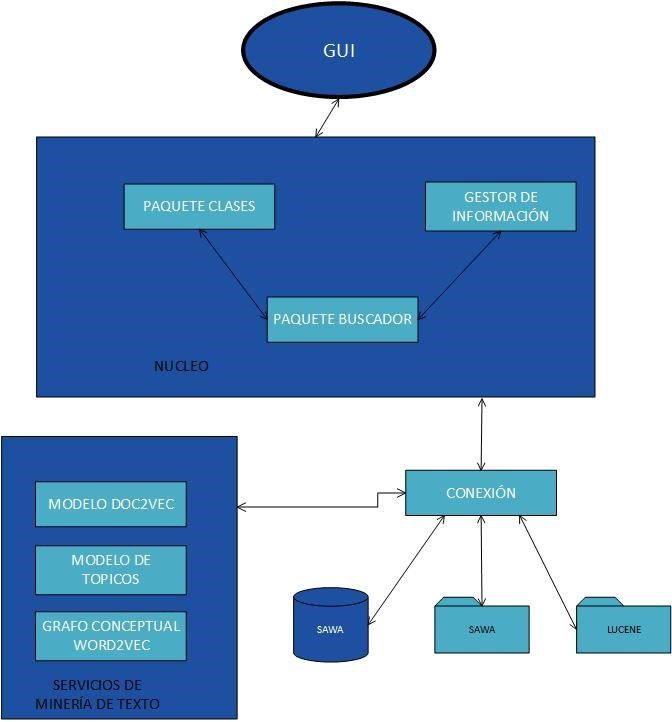
\includegraphics[width=0.9\textwidth]{implementacion1.png}
%\caption{Arquitectura de Maskana.}
%\label{fig:implementacion1}
%\end{figure}
%
%\textbf{Módulo de Servicios de Minería de texto.}
%
%Este módulo es el encargado de brindar servicios web que conectan a Maskana con los modelos elaborados en la sección de modelado, en este módulo
% se encuentran los algoritmos para relacionar documentos conceptualmente,
% conocer los temas o tópicos principales de los trabajos de grado consultados y sus relaciones.
% A continuación, se hace una descripción de los submódulos que lo componen.
%
%\textbf{Modelo Doc2vec:}
%Este submódulo lleva el nombre del modelo Doc2vec,el cual se encarga de realizar la representación vectorial de todos los documentos del repositorio, generando vectores conceptuales teniendo en cuenta el contexto de los documentos con los que fue entrenado, estos vectores están almacenados en la base de datos Sawa mediante el módulo de conexión, 
%se implementó el algoritmo \ref{alg:maskanita1} , el cual permite  encontrar similitudes conceptuales entre los documentos del repositorio; ayudando a extender las búsquedas que realizan los usuarios de la herramienta Maskana.
%
%\begin{algorithm}
%    \renewcommand{\algorithmicrequire}{\textbf{Input:}}
%    \renewcommand{\algorithmicrequire}{\textbf{Input:}}
%    \renewcommand{\algorithmicensure}{\textbf{Output:}}
%    \renewcommand{\algorithmicprint}{\textbf{break}}
%  \caption{ Maskanita recomendación de trabajos de grado.}
%  \label{alg:maskanita1}
%  \algsetup{indent=2em}
%  \footnotesize
%  \begin{algorithmic}[1]
%\REQUIRE {D: documento resultado de búsqueda} 
%\REQUIRE {Corpus\_doc2vec : corpus estructurados con el modelo doc2veca} 
%\ENSURE {DocRel: conjunto de documentos relacionados a D}
%\STATE $DocRel \leftarrow \emptyset$
%\STATE vector\_documento=doc2vec(D)
%\STATE grupo\_documento=xgboost.clasificar(vector\_documento)
%\FOR {each doc  \in$ Corpus\_doc2vec  \in$  grupo\_documento }
%	\IF{ similitud\_coseno( vector\_documento,doc2vec(doc))>0.7}
%		  \STATE {DocRel $\leftarrow $adicionar(DocRel,doc) }
%		% \STATE {D $\leftarrow$ points $\in c$ }
%	\ENDIF
%\ENDFOR
%\STATE {ordenar(DocRel) }
%\end{algorithmic}
%\end{algorithm}
%
%%\begin{figure}[H]
%%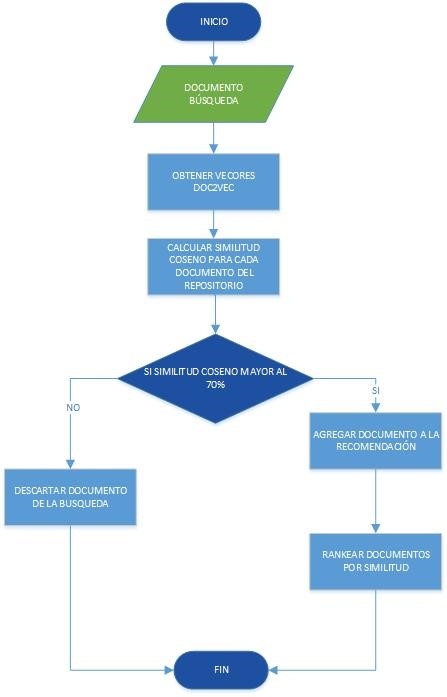
\includegraphics[width=0.7\textwidth]{implementacion2}
%%\caption{Diagrama de flujo algoritmo Maskanita recomendación de trabajos de grado.}
%%\label{fig:implementacion2}
%%\end{figure}
%
%\textbf{Modelo de tópicos:} En este submódulo se encuentra implementado el algoritmo LDA para conocer los diferentes tópicos 
%o temas relacionados con los trabajos de grado, recomendados por el algoritmo Maskanita. Como primer paso se toma los documentos recomendados por el algoritmo Maskanita, como segundo paso 
%se obtiene el número de temas a calcular por parte del usuario, seguidamente se ejecuta el algoritmo LDA de la librería Gensim de Python, 
%Finalmente se obtienen los temas principales que componen los documentos recomendados y se los visualiza mediante el servicio web de este submódulo.
%
%\begin{figure}[H]
%\centering
%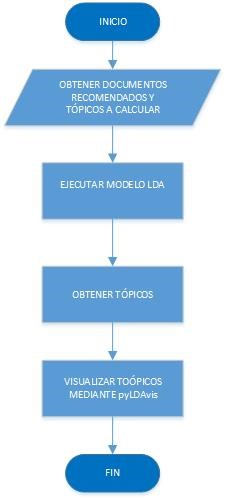
\includegraphics[width=0.3\textwidth]{implementacion3}
%\caption{Proceso submódulo modelo de tópicos.}
%\label{fig:implementacion3}
%\end{figure}
%
%
%\textbf{Grafo conceptual Word2vec:} En este submódulo se encuentra implementado  el algoritmo \ref{alg:maskanita2}, útil para representar relaciones conceptuales del contenido de los trabajos de grado recomendados por el algoritmo Maskanita  \ref{alg:maskanita1}. 
%El primer paso toma como entrada los documentos recomendados por Maskanita \ref{alg:maskanita1}, En segundo lugar, se obtiene conceptos relevantes de los documentos de entrada mediante la tarea de reconocimiento de entidades nombradas de la librería Spacy de Python,
%Para cada entidad o concepto reconocido se aplica el modelo Word2vec para conocer sus relaciones, finalmente se construye el grafo conceptual usando la librería D3.js y  el servicio web implementado en este submódulo.  
%
%
%\begin{algorithm}
%    \renewcommand{\algorithmicrequire}{\textbf{Input:}}
%    \renewcommand{\algorithmicensure}{\textbf{Output:}}
%    \renewcommand{\algorithmicprint}{\textbf{break}}
%  \caption{ Maskanita relaciones conceptuales de trabajos de grado.}
%  \label{alg:maskanita2}
%  \algsetup{indent=2em}
%  \footnotesize
%  \begin{algorithmic}[1]
%\REQUIRE {T: contenido textual documentos relacionados } 
%\ENSURE {G: Grafo Conceptual }
%\STATE $conceptos\_ner \leftarrow \emptyset$
%\STATE $G \leftarrow \emptyset$
%\STATE {spacy.load('es\_core\_news\_sm') }
%\FOR {each token  \in$ T }
%	\IF{spacy.isNer(token)}
%		  \STATE {$conceptos\_ner $\leftarrow $adicionar(conceptos\_ner,token)}
%		% \STATE {D $\leftarrow$ points $\in c$ }
%	\ENDIF
%\ENDFOR
%
%\FOR {each c  \in$ conceptos\_ner }
%	\FOR {rl  \in$  word2vec.sim(c) }
%		  \STATE {$n1 $\leftarrow $crearNodo(c)}
%		  \STATE {$n2 $\leftarrow $crearNodo(rl)}
%		  \STATE {$G $\leftarrow $relacionarNodos(n1,n2)}
%	\ENDFOR
%\ENDFOR
%
%
%\end{algorithmic}
%\end{algorithm}

%%%%%%%%%%%%%%%%%%%%%%%%%%
















\chapter{Resultados}

Este capítulo muestra los resultados obtenidos en cada fase de la metodología de esta investigación.

\section{Comprensión del problema y preparación de los datos}

En la fase de comprensión del problema se obtuvo  un marco teórico referente a todas las técnicas utilizadas en esta investigación para tratar con documentos textuales no estructurados.
En la fase de  preparación de los datos se obtuvo un corpus limpio compuesto por 10.000 documentos.

\section{Modelado}

En esta fase se obtuvieron modelos para estructurar los documentos y modelos de aprendizaje supervisado y no supervisado para identificar áreas de conocimiento en los trabajos de grado .

\textbf{Modelos para estructurar el corpus}

La tabla \ref{tab:ProgramasDM} muestra el estadístico de Hopkins para cada conjunto de datos generado. 


\begin{table}[H]\centering
	\caption{Descripción de la tendencia al agrupamiento en los conjuntos de datos.}\label{tab:ProgramasDM}
	\begin{tabularx}{\textwidth}{XXXm{6.0cm}}\toprule

Modelo &  \multicolumn{1}{c}{Estadístico Hopkins} & \multicolumn{1}{c}{Descripción} \\ 
Bow & 0.61 & Modelo Bow generando un conjunto de datos de 10.000 filas * 20.000 
columnas usando unigramas y bigramas.
Este método descarta términos que aparezcan en más del 70\% de documentos.  \\ 
Bow &  0.58 & Modelo Bow generando un conjunto de datos de 10.000 filas * 10.000 
columnas usando unigramas y bigramas.
Este método descarta términos que aparezcan en más del 70\% de documentos.   \\ 
Tf-idf & 0.54 & Modelo Tf-id generando un conjunto de datos de 10.000 filas * 20.000 
columnas usando unigramas y bigramas.
Este método descarta términos que aparezcan en más del 70\% de documentos.  \\ 
Tf-idf &  0.52 & Modelo Tf-id generando un conjunto de datos de 10.000 filas * 10.000 
columnas usando unigramas y bigramas.
Este método descarta términos que aparezcan en más del 70\% de documentos.   \\ 
Doc2vec & 0.38 & Este método representa un documento mediante 
un vector de tamaño 20
usando el algoritmo bolsa de palabras distribuida  (PV-DBOW)   \\ 
Doc2vec & 0.42  & Este método representa un documento mediante
un vector de tamaño 20
usando el algoritmo memoria distribuida (PV-DM) \\  \bottomrule
	\end{tabularx}

\end{table}

Con un umbral establecido en 0.5 podemos confirmar que existe tendencia al agrupamiento en los conjuntos de datos generados por los modelos Doc2vec bolsa de palabras distribuida (PV-DBOW) y Doc2vec memoria distribuida (PV-DM).
%Los resultados muestran una mejor tendencia al agrupamiento en los modelos Doc2vec,
Los modelos Doc2vec  logran captar relaciones conceptuales mediante el contexto que representa cada documento, usando esta representación se podrá medir qué tan relacionado está un documento con respecto a los demás.	

%%%%%%%%%%%%%%%%%%%%%%%%%%%%%%%%%%%%%%%%%%%%%%%%%%%%%%%%%%%%
\textbf{Modelos de aprendizaje automático  }

Con el fin de descubrir grupos de conocimiento de acuerdo al contexto de los diferentes trabajos de grado se corrió el algoritmo k-medias.

Para la selección del k óptimo generamos diferentes grupos iterando k desde 20 a 44 evaluando el coeficiente de Silhouette y el error cuadrático en los 2 conjuntos de datos generados con el modelo Doc2vec ya que tienen tendencia al agrupamiento.


\begin{figure}[H]
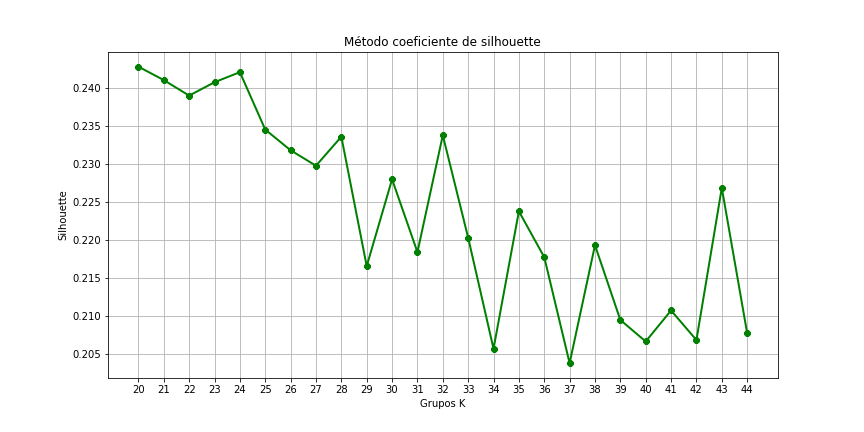
\includegraphics[width=1\textwidth]{Silhouette}
\caption{Método coeficiente de Silhouette algoritmo Kmedias }
\label{fig:proceso3}
\end{figure}

\begin{figure}[H]
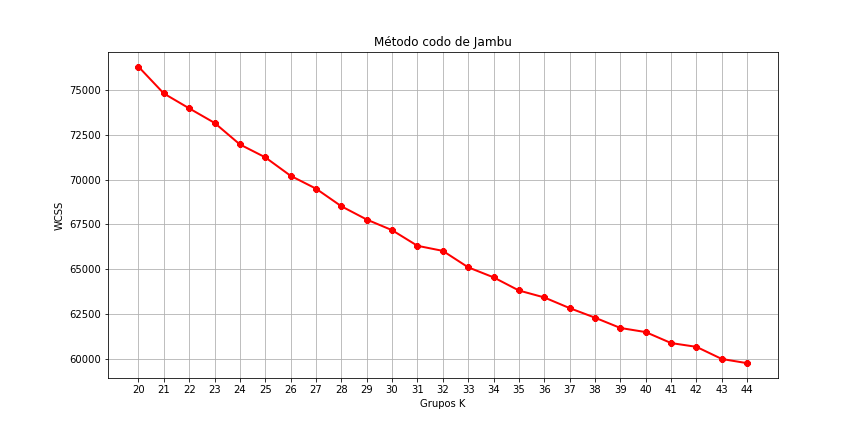
\includegraphics[width=1\textwidth]{WCSS}
\caption{Método de codo de Jambu algoritmo Kmedias}
\label{fig:proceso4}
\end{figure}

En la figura  \ref{fig:proceso3} se visualiza el método de coeficiente de Silhouette; el cual sugiere que el número adecuado de grupos es de 24, en la figura  \ref{fig:proceso4} se visualiza el método del codo de Jambu; 
para el cual miramos que a medida que k se incrementa la distancia de los puntos al centroide va disminuyendo. Para la selección del K óptimo  se contrasto los dos métodos y se eligió el k en 32; ya que miramos que su coeficiente de Silhouette está entre los más altos y a la vez la distancia de los puntos al centroide es baja. Por lo tanto se corrió el algoritmo k medias con k =32, con el fin de clasificar los documentos en 32 áreas de conocimiento de acuerdo a su temática de contexto. Para clasificar futuros trabajos de grado en los grupos encontrados se entrenó modelos de aprendizaje supervisado; los cuales se verán en el capítulo de discusión.



%%%%%%%%%%%%%%%%%%%%%%%%%%%%%%%%%%%%%%%%%%%%%%%%%%%%%%%%%%%%%%%%%

\section{Implementación}


Maskana está compuesta por 3 módulos: el módulo GUI, el módulo núcleo y el módulo de conexión. En esta fase se presenta el cuarto módulo denominado servicios de minería de texto, el cual se puede observar en la figura \ref{fig:implementacion1}.


\begin{figure}[H]
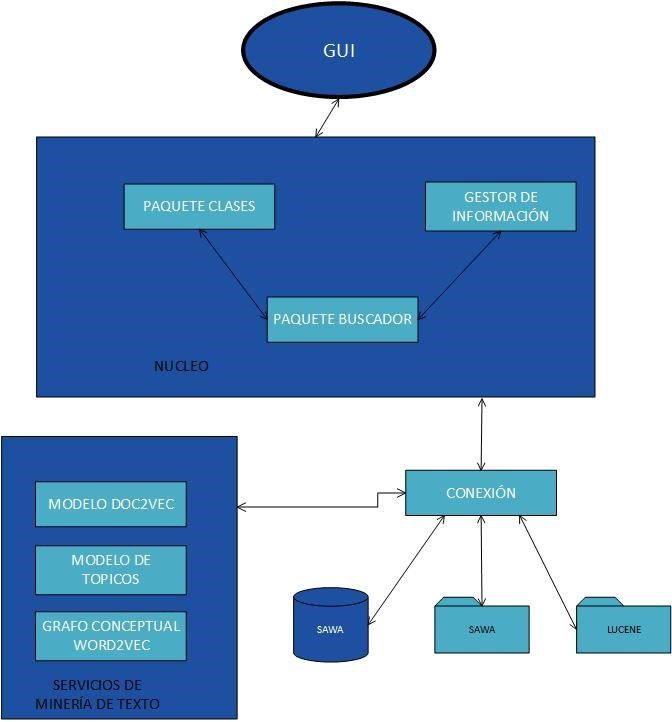
\includegraphics[width=0.9\textwidth]{implementacion1.png}
\caption{Arquitectura de Maskana.}
\label{fig:implementacion1}
\end{figure}

\textbf{Módulo de Servicios de Minería de texto.}

Este módulo es el encargado de brindar servicios web que conectan a Maskana con los modelos elaborados en la sección de modelado, en este módulo
 se encuentran los algoritmos para relacionar documentos conceptualmente,
 conocer los temas o tópicos principales de los trabajos de grado consultados y sus relaciones.
 A continuación, se hace una descripción de los submódulos que lo componen.

\textbf{Modelo Doc2vec:}
Este submódulo lleva el nombre del modelo Doc2vec,el cual se encarga de realizar la representación vectorial de todos los documentos del repositorio, generando vectores conceptuales teniendo en cuenta el contexto de los documentos con los que fue entrenado, estos vectores están almacenados en la base de datos Sawa mediante el módulo de conexión, 
se implementó el algoritmo \ref{alg:maskanita1} , el cual permite  encontrar similitudes conceptuales entre los documentos del repositorio; ayudando a extender las búsquedas que realizan los usuarios de la herramienta Maskana.

\begin{algorithm}
    \renewcommand{\algorithmicrequire}{\textbf{Input:}}
    \renewcommand{\algorithmicrequire}{\textbf{Input:}}
    \renewcommand{\algorithmicensure}{\textbf{Output:}}
    \renewcommand{\algorithmicprint}{\textbf{break}}
  \caption{ Maskanita recomendación de trabajos de grado.}
  \label{alg:maskanita1}
  \algsetup{indent=2em}
  \footnotesize
  \begin{algorithmic}[1]
\REQUIRE {D: documento resultado de búsqueda} 
\REQUIRE {Corpus\_doc2vec : corpus estructurados con el modelo doc2veca} 
\ENSURE {DocRel: conjunto de documentos relacionados a D}
\STATE $DocRel \leftarrow \emptyset$
\STATE vector\_documento=doc2vec(D)
\STATE grupo\_documento=xgboost.clasificar(vector\_documento)
\FOR {each doc  \in$ Corpus\_doc2vec  \in$  grupo\_documento }
	\IF{ similitud\_coseno( vector\_documento,doc2vec(doc))>0.7}
		  \STATE {DocRel $\leftarrow $adicionar(DocRel,doc) }
		% \STATE {D $\leftarrow$ points $\in c$ }
	\ENDIF
\ENDFOR
\STATE {ordenar(DocRel) }
\end{algorithmic}
\end{algorithm}

El algoritmo \ref{alg:maskanita1} implementado en Maskana permite realizar búsquedas temáticas y recomendaciones de trabajos relacionados contextualmente con otros. 
Como entrada se envía la consulta o un documento del repositorio,
el modelo Doc2vec se encarga de realizar la representación vectorial de la entrada,
el modelo Xgboost se encarga de clasificar el vector generado en los dominios o grupos encontrados; para filtrar el resultado al dominio clasificado y obtener los documentos que tengan  mayor similitud conseno.


%\begin{figure}[H]
%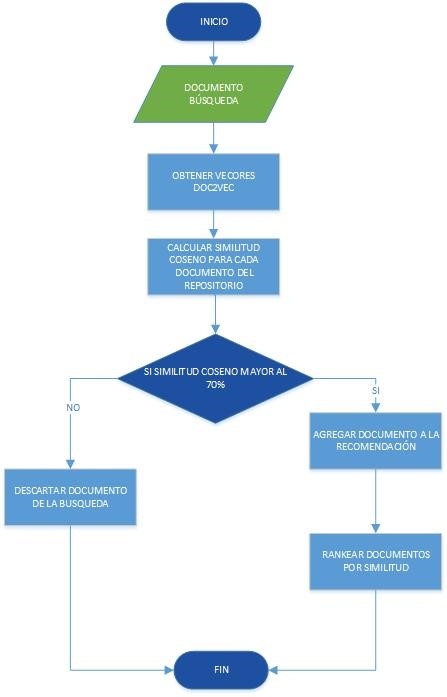
\includegraphics[width=0.7\textwidth]{implementacion2}
%\caption{Diagrama de flujo algoritmo Maskanita recomendación de trabajos de grado.}
%\label{fig:implementacion2}
%\end{figure}

\textbf{Modelo de tópicos:} En este submódulo se encuentra implementado el algoritmo LDA para conocer los diferentes tópicos 
o temas relacionados con los trabajos de grado, recomendados por el algoritmo Maskanita. Como primer paso se toma los documentos recomendados por el algoritmo Maskanita, como segundo paso 
se obtiene el número de temas a calcular por parte del usuario, seguidamente se ejecuta el algoritmo LDA de la librería Gensim de Python, 
Finalmente se obtienen los temas principales que componen los documentos recomendados y se los visualiza mediante el servicio web de este submódulo.

\begin{figure}[H]
\centering
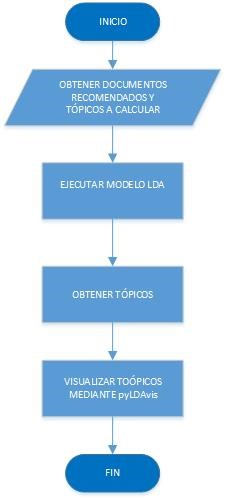
\includegraphics[width=0.3\textwidth]{implementacion3}
\caption{Proceso submódulo modelo de tópicos.}
\label{fig:implementacion3}
\end{figure}


\textbf{Grafo conceptual Word2vec:} En este submódulo se encuentra implementado  el algoritmo \ref{alg:maskanita2}, útil para representar relaciones conceptuales del contenido de los trabajos de grado recomendados por el algoritmo Maskanita  \ref{alg:maskanita1}. 
El primer paso toma como entrada los documentos recomendados por Maskanita \ref{alg:maskanita1}, En segundo lugar, se obtiene conceptos relevantes de los documentos de entrada mediante la tarea de reconocimiento de entidades nombradas de la librería Spacy de Python,
Para cada entidad o concepto reconocido se aplica el modelo Word2vec para conocer sus relaciones, finalmente se construye el grafo conceptual usando la librería D3.js y  el servicio web implementado en este submódulo.  


\begin{algorithm}[H]
    \renewcommand{\algorithmicrequire}{\textbf{Input:}}
    \renewcommand{\algorithmicensure}{\textbf{Output:}}
    \renewcommand{\algorithmicprint}{\textbf{break}}
  \caption{ Maskanita relaciones conceptuales de trabajos de grado.}
  \label{alg:maskanita2}
  \algsetup{indent=2em}
  \footnotesize
  \begin{algorithmic}[1]
\REQUIRE {T: contenido textual documentos relacionados } 
\ENSURE {G: Grafo Conceptual }
\STATE $conceptos\_ner \leftarrow \emptyset$
\STATE $G \leftarrow \emptyset$
\STATE {spacy.load('es\_core\_news\_sm') }
\FOR {each token  \in$ T }
	\IF{spacy.isNer(token)}
		  \STATE {$conceptos\_ner $\leftarrow $adicionar(conceptos\_ner,token)}
		% \STATE {D $\leftarrow$ points $\in c$ }
	\ENDIF
\ENDFOR

\FOR {each c  \in$ conceptos\_ner }
	\FOR {rl  \in$  word2vec.sim(c) }
		  \STATE {$n1 $\leftarrow $crearNodo(c)}
		  \STATE {$n2 $\leftarrow $crearNodo(rl)}
		  \STATE {$G $\leftarrow $relacionarNodos(n1,n2)}
	\ENDFOR
\ENDFOR


\end{algorithmic}
\end{algorithm}


%%%%%%%%%%%%%%%%%%%%%%%%%%%%%%%%%%%%%%%%%%%%%%%%%%%%%%%%%%%%%%%%%%



\textbf{Interpretación de las categorías  mediante grafos conceptuales.}

%En esta sección se interpreta el conocimiento obtenido mediante grafos conceptuales, los cuales permiten visualizar relaciones conceptuales temáticas; organizando contextualmente el corpus de trabajos de grado; soportadas por el modelo Word2vec, estos fueron elaborados para trabajos de grado relacionados encontrados en diferentes áreas de conocimiento de cada grupo formado.
%En la figura \ref{fig:procesocinco} se observa la distribución de los diferentes documentos del repositorio; estructurados por el modelo Doc2vec con su respectivo grupo en coordenadas de las componentes principales. A continuación, se interpreta cada grupo y los dominios de conocimiento que representan.

En este apartado se  se interpreta el conocimiento obtenido en cada grupo de conocimiento encontrado mediante grafos conceptuales creados por el algoritmo \ref{alg:maskanita2},
el cual permite visualizar relaciones conceptuales temáticas;

En la figura \ref{fig:procesocinco} se observa la distribución de los diferentes documentos del repositorio; estructurados por el modelo Doc2vec con su respectivo grupo en coordenadas de las componentes principales.


\begin{figure}[H]
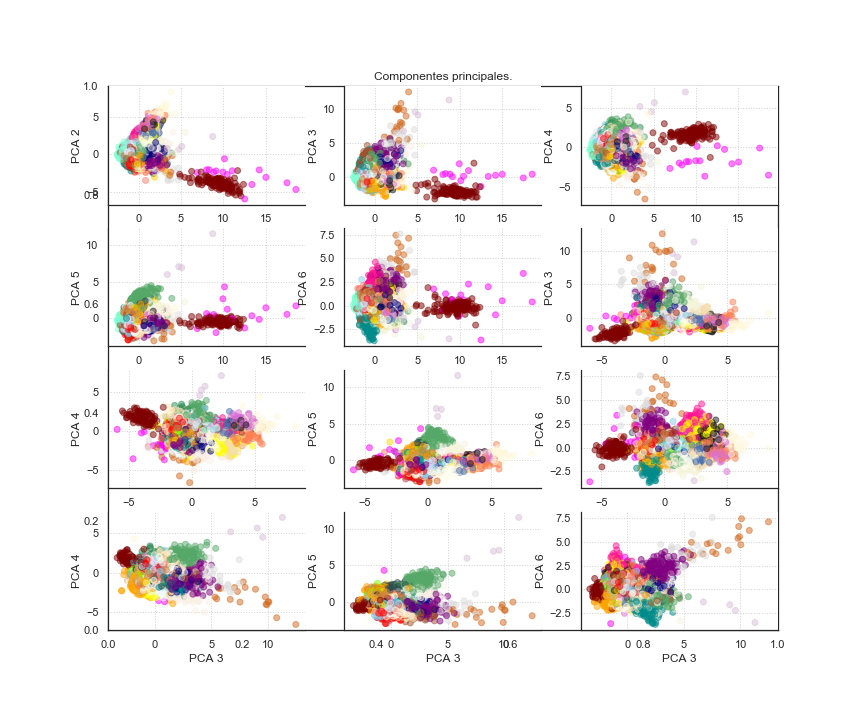
\includegraphics[width=1\textwidth]{proceso5}
\caption{Biplot componentes principales}
\label{fig:procesocinco}
\end{figure}


\begin{table}[H]\centering
\caption{Resumen grupos}\label{tab:tablaeg}
	\begin{tabularx}{\textwidth}{XXXm{3.0cm}}\toprule

Grupo &  \multicolumn{1}{c}{Cantidad } \\ 
0&      309\\
1&     382\\
2&     346\\
3&    409\\
4&   137\\
5&   175\\
6&   159\\
7&   456\\
8&   341\\
9&   389\\
10& 30\\
11& 158\\
12& 510\\
13& 237\\
14& 317\\
15& 206\\
16& 230\\
17& 145\\
18& 137\\
19& 353\\
20& 282\\
21& 126\\
22& 344\\
23& 68\\
24& 226\\
25& 192\\
26& 87\\
27& 374\\
28& 326\\
29& 233\\
30& 211\\
31& 181\\


 \bottomrule
	\end{tabularx}
	
\end{table}

 La tabla  \ref{tab:tablaeg}  indica cuántos trabajos quedaron en cada cluster, a continuación, se interpreta cada grupo y los dominios de conocimiento que representan.

En el grupo 0 se encuentran trabajos relacionados a temáticas respectivas a los derechos humanos, derechos constitucionales, derechos laborales, derechos penales, derecho judicial, derecho administrativo, leyes y artículos constitucionales.

En el grupo 1 se encuentran trabajos de grado relacionados a temáticas de desempleo, desigualdad social , condiciones socioeconómicas, fortalecimiento del comercio y economía. 

En el grupo 2 se encuentran trabajos relacionados a temáticas de relaciones interfamiliares, estudios de violencia, conflictos familiares, machismo, patriarcado y problemáticas dentro del contexto sociológico como describe la figura \ref{fig:grupo14}.
\begin{figure}[H]\centering
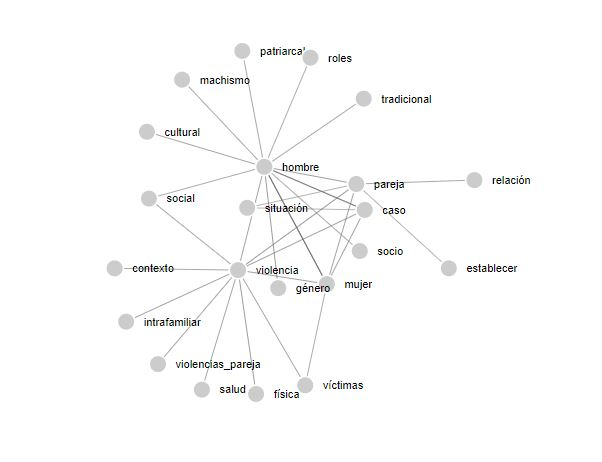
\includegraphics[width=0.8\textwidth]{grupo14}
%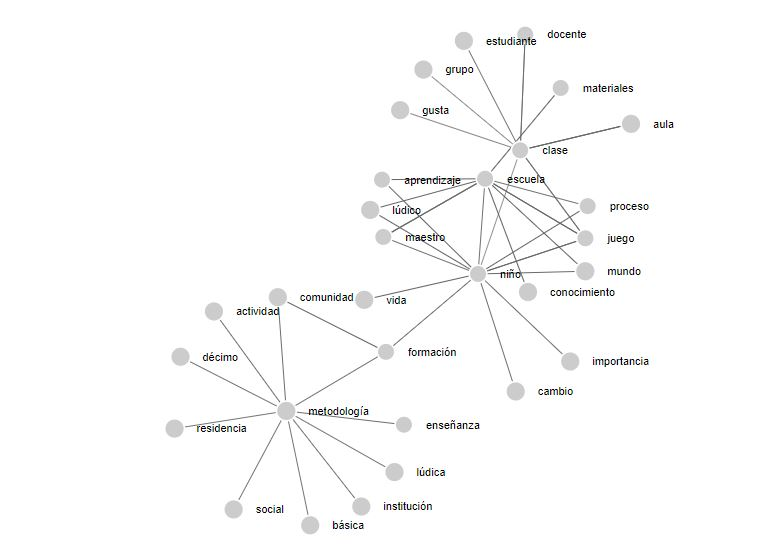
\includegraphics[width=0.8\textwidth]{grupo8}
\caption{Grafo  relaciones temáticas grupo 2 }
\label{fig:grupo14}
\end{figure}

%En el grupo 8 se encuentran trabajos relacionados con temáticas pedagógicas para la educación básica primaria. 
%\begin{figure}[H]\centering
%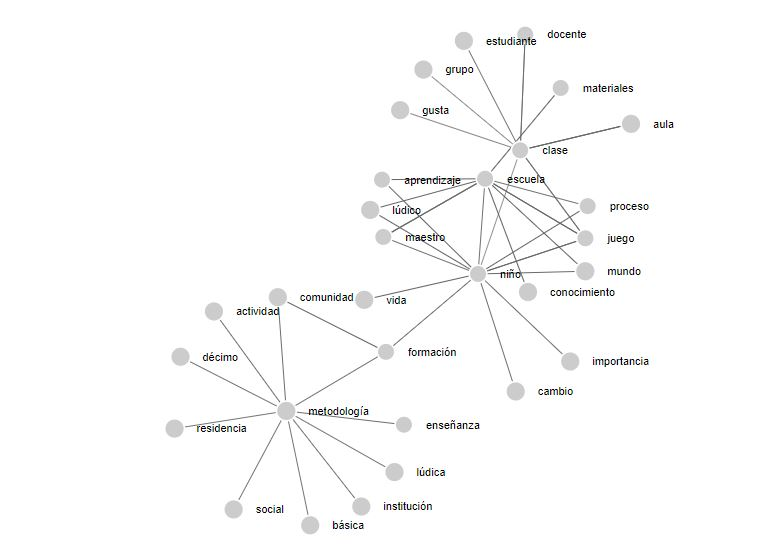
\includegraphics[width=0.8\textwidth]{grupo8}
%\caption{Grafo  relaciones temáticas  grupo 8 }
%\label{fig:grupo8}
%\end{figure}

%En la figura \ref{fig:grupo14} podemos observar relaciones contextuales complementarias del grupo 8 tales como: escuela, maestros , aulas de clase, estrategias y metodologías didácticas de aprendizaje basadas en lúdicas y juegos para niños estudiantes de básica  primaria.

En el grupo 3 se encuentran trabajos de grado relacionados a temáticas de planeación estratégica empresarial, marketing y estudios de comercio en  organizaciones, como se puede observar en la figura \ref{fig:grupo5} .
\begin{figure}[H]\centering
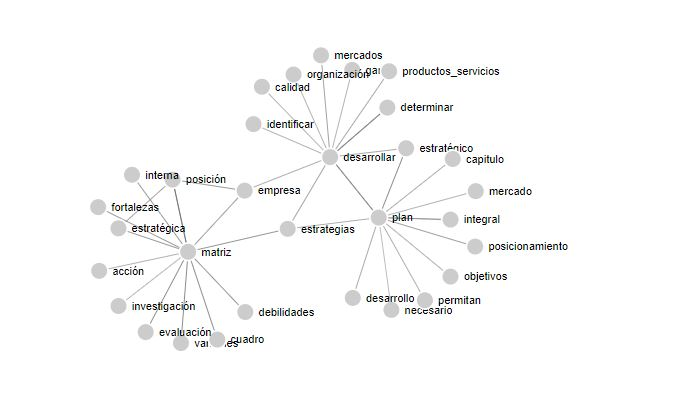
\includegraphics[width=1\textwidth]{grupo5}
\caption{Grafo relaciones temáticas grupo 3 }
\label{fig:grupo5}
\end{figure}

En el grupo 4 se encuentran trabajos de grado relacionados al departamento de idiomas, todos los documentos de este grupo se encuentran en idioma inglés, reprentado en la figura \ref{fig:grupo6}.

\begin{figure}[H]\centering
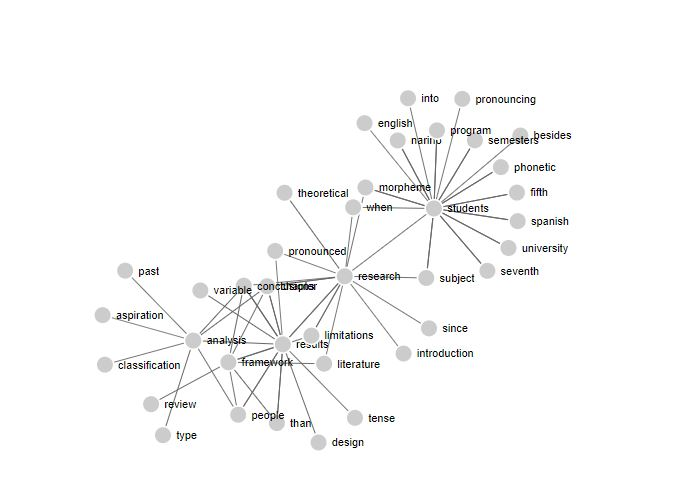
\includegraphics[width=0.8\textwidth]{grupo6}
\caption{Grafo  relaciones temáticas grupo 4 }
\label{fig:grupo6}
\end{figure}

En el grupo 5 se encuentran trabajos de grados vinculados a la facultad de ciencias exactas, específicamente al programa de Biología, evaluando diferentes tratamientos para encontrar diferencias estadísticamente significativas entre estos y así mejorar el crecimiento y producción de especies. %%

En el grupo 6 se encuentran trabajos relacionados al estudio de modelamiento de fluidos.

En el grupo 7 se encuentran trabajos de grado relacionados a temas de cultura, carnavales, historia y desarrollo social.
\begin{figure}[H]\centering
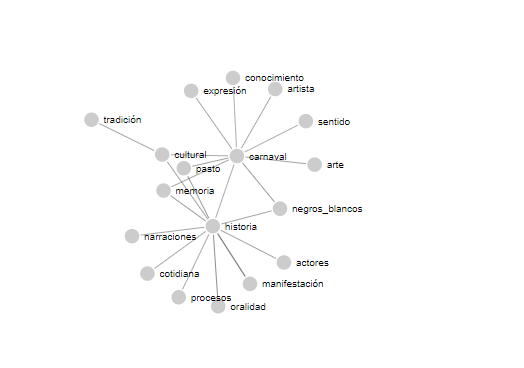
\includegraphics[width=0.8\textwidth]{grafocul0}
\caption{Grafo  relaciones temáticas grupo 7 }
\label{fig:grafoculcero}
\end{figure}



La figuera \ref{fig:grafoculcero}  se muestra el grafo  conceptual  de los trabajos de grado clasificados en el grupo 7, donde se observa conceptos relacionados referentes al carnaval de negros y blancos, cultura, artes , maestros y artesanos.

En el grupo 8 se encuentran trabajos relacionados a construcción, desarrollo, gestión de calidad y auditoría de obras civiles.

En el grupo 9 se encuentran trabajos de grado relacionados con temáticas pedagógicas de aprendizaje   y estrategias lúdicas de aprendizaje  para estudiantes.

En el grupo 10 se encuentran trabajos de grado relacionados específicamente a ingeniería de software, lenguaje unificado de modelado UML, desarrollo y construcción de módulos y sistemas de información a la medida.

En el grupo 11 se encuentran trabajos relacionados a telemática, microcontroladores, reconocimiento de imágenes, redes neuronales ,  espectro electromagnético,  series temporales,  aplicaciones en vulcanología y sismología. 

En el grupo 12 se encuentran trabajos de grado vinculados al programa de ingeniería agroindustrial referentes a temáticas de desarrollo, comercialización, industrialización, estudios de oferta y demanda de productos agropecuarios.

En el grupo 13 se encuentran trabajos de grado en temáticas de ordenamiento territorial, desarrollo sostenible y seguridad social.  %%%%%

En el grupo 14 se encuentran trabajos de grado relacionados con proyectos referentes a entornos y herramientas virtuales de aprendizaje.

En el grupo 15 se encuentran trabajos de grado vinculados a esquemas de seguridad, salud ocupacional en la industria y riesgos laborales como se describe en la figura \ref{fig:grupo22}


\begin{figure}[H]\centering
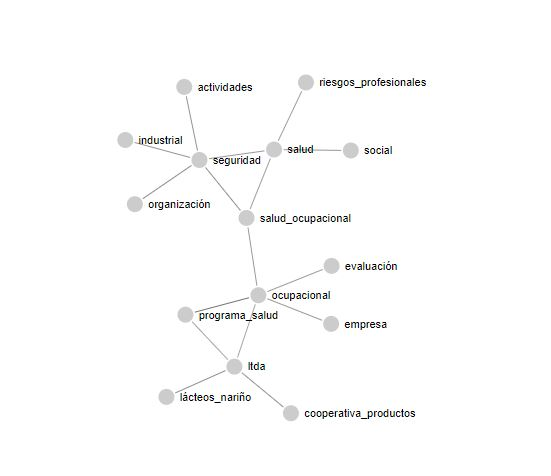
\includegraphics[width=0.8\textwidth]{grupo22}
\caption{Grafo  relaciones temáticas grupo 15}
\label{fig:grupo22}
\end{figure}


En el grupo 16 se encuentran trabajos de grado relacionados a cultivos, recursos hídricos  , plantas, especies y temáticas agroforestales como se observa en la figura \ref{fig:grupo1especies}.
\begin{figure}[H]\centering
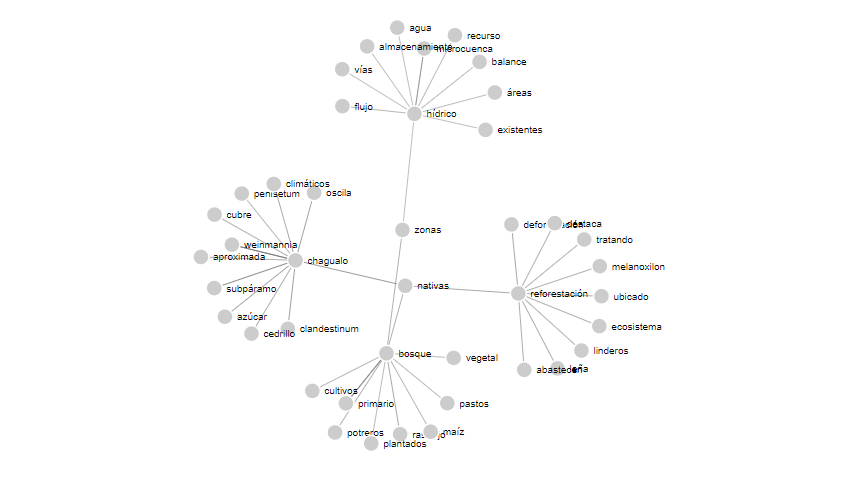
\includegraphics[width=1\textwidth]{grupo1especies}
\caption{Grafo relaciones temáticas grupo 16 }
\label{fig:grupo1especies}
\end{figure}

El grupo 17 contiene tópicos relacionados con bacterias, microorganismos, compuestos antioxidantes, proteínas y aminoácidos como se describe en la figura \ref{fig:grupo25}.
\begin{figure}[H]\centering
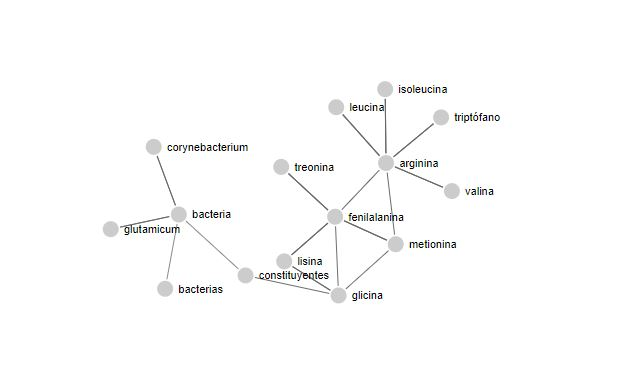
\includegraphics[width=0.8\textwidth]{grupo25}
\caption{Grafo  relaciones temáticas grupo 17}
\label{fig:grupo25}
\end{figure}

En el grupo 18 se encuentran trabajos relacionados con temáticas temáticas afines a administración, economía y finanza empresarial.

En el grupo 19 se encuentran trabajos relacionados a temáticas sociales, desarrollo humano sostenible, desarrollo económico social, derecho internacional humanitario y políticas comunitarias.

En el grupo 20 se encuentran trabajos de grado de la facultad de artes, referentes a temáticas culturales, artesanías e  historia del arte.

En el grupo 21 se encuentran trabajos relacionados a la facultad de ciencias económicas y administrativas los cuales involucran temáticas de comercio exterior, aduanas, exportaciones, impuestos, empresas, fiscalización y estudios de mercados.


En el grupo 22 se encuentran trabajos de grado relacionados con planes de ordenamiento  territorial   y ecoturismo tal como se observa en la figura \ref{fig:ordenaminetoimg}.


\begin{figure}[H]\centering
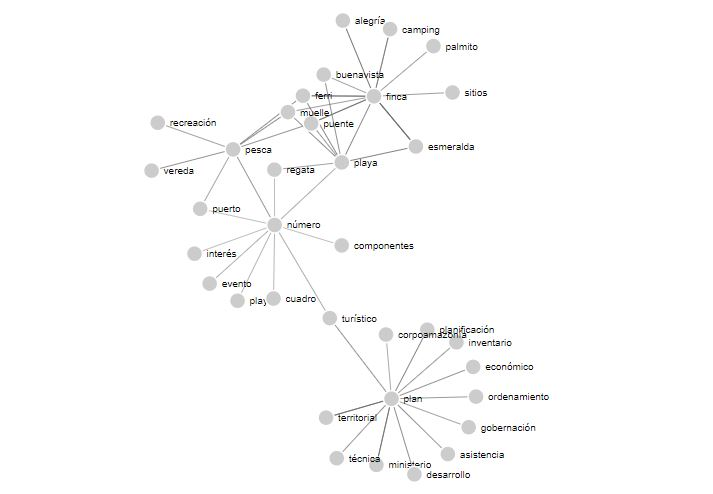
\includegraphics[width=1\textwidth]{ordenaminetoimg}
\caption{Grafo relaciones temáticas grupo 22 }
\label{fig:ordenaminetoimg}
\end{figure}

En el grupo 23 se encuentran trabajos de grado de la facultad de ciencias agrícolas, específicamente del programa de ingeniería agronómica, relacionando temáticas referentes a estudios de variedades de especies de granos, tubérculos, plantas y técnicas de comparación de diferentes tratamientos agronómicos mediante pruebas de Tukey y validaciones estadísticas
como se representa en la figura \ref{fig:grupo25}.
\begin{figure}[H]\centering
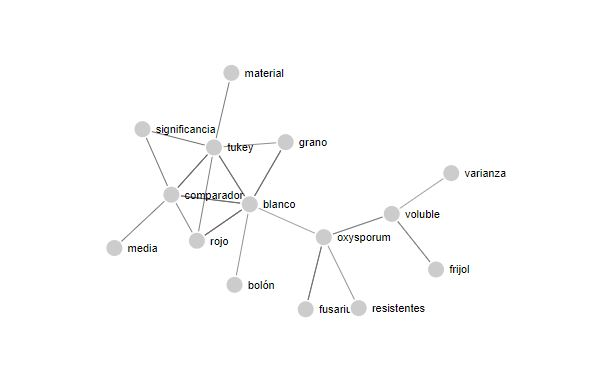
\includegraphics[width=0.8\textwidth]{grupo28}
\caption{Grafo  relaciones temáticas grupo 23}
\label{fig:grupo25}
\end{figure}


En el grupo 24 se encuentran trabajos relacionados con medicina veterinaria, en la figura \ref{fig:grupo7} se aprecia relaciones entre enfermedades causadas por las bacterias babesia y  anaplasma en equinos.

\begin{figure}[H]\centering
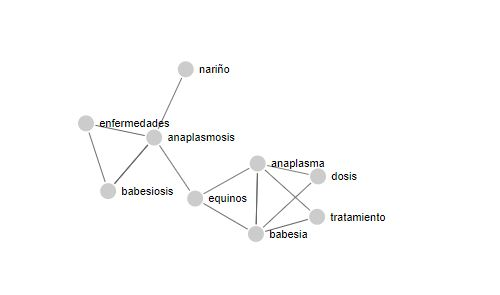
\includegraphics[width=0.8\textwidth]{grupo7}
\caption{Grafo  relaciones temáticas grupo 24 }
\label{fig:grupo7}
\end{figure}

En el grupo 25 se encuentran trabajos de grado relacionados con proyectos de priorización de áreas ambientales, caracterización de sistemas agroforestales, investigación de especies y reservas naturales.  %%

En el grupo 26 se encuentran trabajos de grado relacionados con música.

En el grupo 27 se encuentran trabajos relacionados con temáticas pedagógicas para la educación. 
\begin{figure}[H]\centering
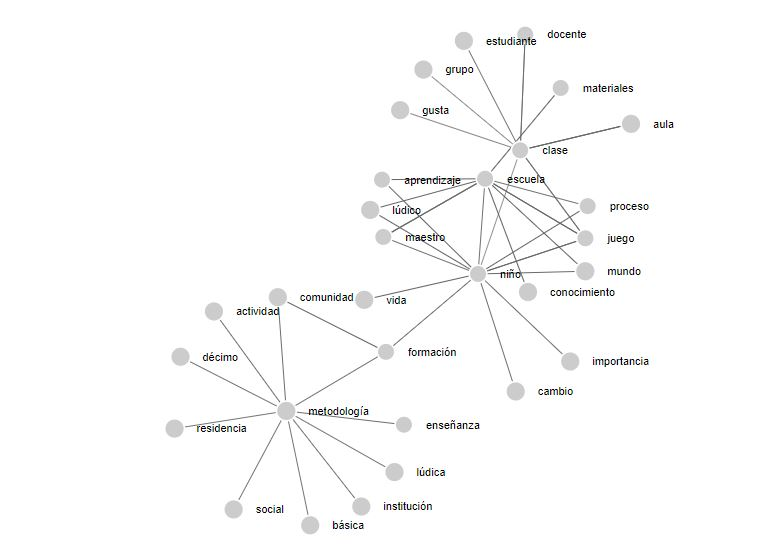
\includegraphics[width=0.8\textwidth]{grupo8}
\caption{Grafo  relaciones temáticas grupo 27 }
\label{fig:grupo8}
\end{figure}

En la figura \ref{fig:grupo8} podemos observar relaciones contextuales complementarias del grupo 27 tales como: escuela, maestros , aulas de clase, estrategias y metodologías didácticas de aprendizaje basadas en lúdicas y juegos para niños estudiantes de básica  primaria.

En el grupo 28 se encuentran trabajos de grado relacionados al programa de administración empresas, referentes a estudios del clima organizacional, talento humano, selección de personal, control interno y procesos de gestión y calidad en las empresas.

En el grupo 29 se encuentran trabajos de grado del programa de Psicología, relacionados con factores de riesgo en adolencetes causantes de suicidio, identificación de ideas suicidas como se describe en la figura \ref{fig:grupo14}.
\begin{figure}[H]\centering
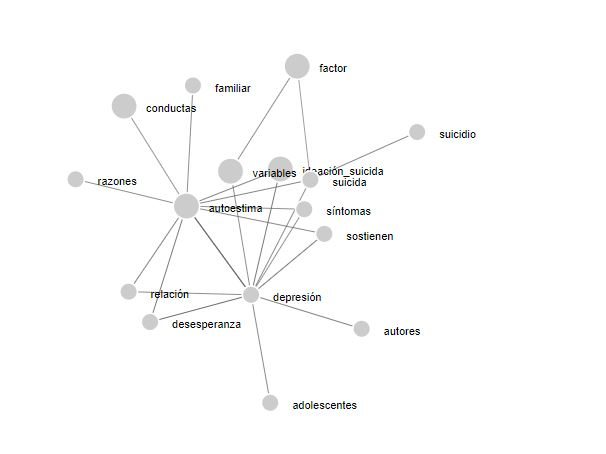
\includegraphics[width=0.8\textwidth]{grupo19}
\caption{Grafo  relaciones temáticas grupo 29 }
\label{fig:grupo19}
\end{figure}

En el grupo 30 se encuentran trabajos relacionados al programa de ingeniería de sistemas, particularmente al área de descubrimiento de conocimiento en base de datos, desarrollo de herramientas bajo el gestor Postgresql, algoritmos de minería de datos, clasificación, agrupación, reglas de asociación y temáticas de software y manejo de información.

\begin{figure}[H]\centering
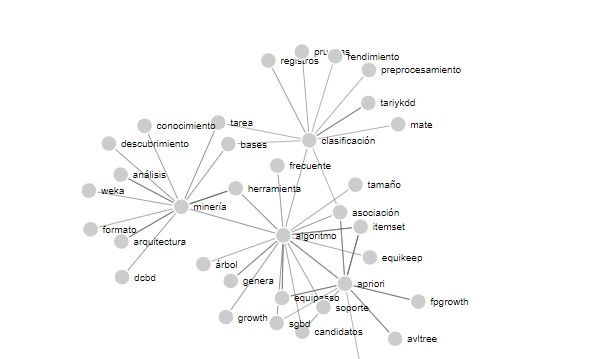
\includegraphics[width=0.8\textwidth]{grafotarykdd}
\caption{Grafo  relaciones temáticas grupo 30 }
\label{fig:tarygradfo}
\end{figure}

En las figuras \ref{fig:tarygradfo}  se muestra el grafo conceptual generado por el modelo Word2vec de los trabajos de grado respectivos al  grupo 30. Donde se pueden establecer vínculos entre conceptos dentro de minería de datos, descubrimiento de conocimiento, algoritmos de clasificación y asociación tales como equipasso, fpgrowth, entrenamiento de  árboles  de decisión, a priori e itemsets frecuentes.

En el grupo 31 se encuentran trabajos de grado relacionados con las ciencias pecuarias, producción acuícola y comparación de dietas en cultivos de peces.



\section{Casos de prueba para trabajos de grado relacionados conceptualmente propuestos por Maskana.}

%Para la evaluación de los trabajos relacionados propuestos por el algoritmo Maskanita \ref{alg:maskanita1}, se realizaron 3 casos de prueba, para los cuales se elaboró una tabla con los resultados obtenidos de las relaciones encontradas para diferentes trabajos de grado, para validar las relaciones propuestas por Maskanita se formaron dos grupos de trabajos; los que fueron relacionados por el algoritmo y los se quedaron por fuera de la frontera de decisión y no se relacionaron, para cada prueba se evalúa el coeficiente de silhouette y se valida la cohesión de los trabajos relacionados y la separación con respecto al grupo de trabajos que no se relacionaron.

Para la evaluación de los trabajos relacionados propuestos por el algoritmo Maskanita \ref{alg:maskanita1}, se realizaron 3 casos de prueba, para los cuales se elaboró una tabla con los resultados obtenidos de las relaciones encontradas para diferentes trabajos de grado.


\begin{table}[H]\centering
\caption{Caso de prueba 1: Resultados recomendación para el trabajo de grado Tariykdd: Una herramienta genérica de descubrimiento de conocimiento en bases de datos débilmente acoplada con el sgbd Postgresql.}\label{tab:tablae1}
	\begin{tabularx}{\textwidth}{XXXm{3.0cm}}\toprule

Id &  \multicolumn{1}{c}{Distancia Milikowski } & \multicolumn{1}{c}{Titulo} \\ 
5268 &0.0006 &Pg\_KDD - Entorno Gráfico para el Sistema de Descubrimiento de 
Conocimiento en Bases de Datos PostgresKDD.   \\ 
446 &  0.0007 &Implantación de primitivas sql para el descubrimiento de reglas de asociación y clasificación al interior del motor del sistema gestor de bases de datos postgresql.   \\ 
183 & 0.0033 &MATE-KDD: Una herramienta genérica para el descubrimiento.   \\ 
4081 &0.0097&EXDACLET: Herramienta de datacleaning basada en agentes inteligentes orientadas a la web \\

 \bottomrule
	\end{tabularx}
	
\end{table}

\begin{table}[H]\centering
\label{tab:tablae1}
	\begin{tabularx}{\textwidth}{XXXm{3.0cm}}\toprule

%Id &  \multicolumn{1}{c}{Distancia Milikowski } & \multicolumn{1}{c}{Titulo} \\ 
4130 & 0.0363  &RASEMUS: Una herramienta para el descubrimiento de conocimiento en bases de datos con técnicas de clustering, débilmente acoplado con el sgbd postgresql. \\ 
6975&0.1320&POLARIS: Herramienta de minería de uso para la web. \\
6206&0.1537&GRFPOSTGRES – Herramienta gráfica para el motor de base de datos postgres.\\
5044&0.1555&STARCUBE: Una herramienta ROLAP de análisis multidimensional para el soporte a la toma de decisiones, débilmente acoplada con el SGBD PostgreSQL. \\
 \bottomrule
	\end{tabularx}
	
\end{table}

%\begin{figure}[H]\centering
%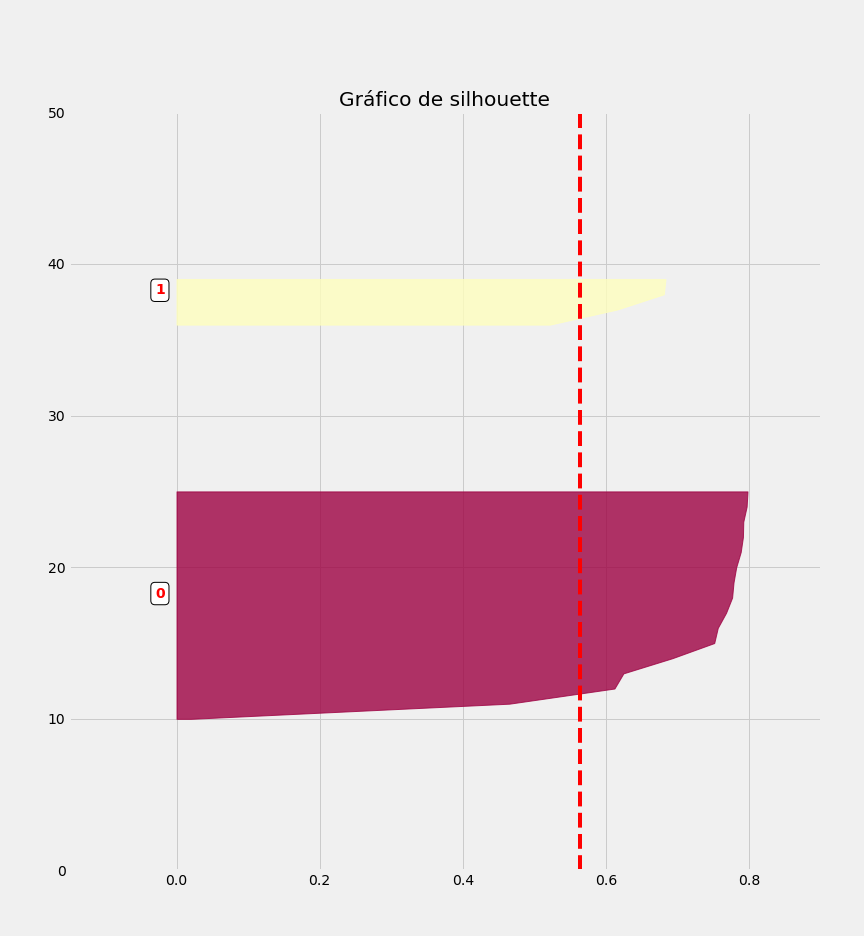
\includegraphics[width=0.8\textwidth]{CoefSil1}
%\caption{Gráfico de Silhouette recomendación caso de prueba 1 }
%\label{fig:silruno}
%\end{figure}




\begin{table}[H]\centering
\caption{Caso de prueba 2: Resultados recomendación para el trabajo de grado Desarrollo e implementación de un sistema de reconocimiento de comandos de voz basado en redes neuronales para la activación de dispositivos electrónicos.}\label{tab:tablae2}
	\begin{tabularx}{\textwidth}{XXXm{3.0cm}}\toprule

Id &  \multicolumn{1}{c}{Distancia Milikowski } & \multicolumn{1}{c}{Titulo} \\ 
5268 &0.0066 &Sistema interactivo de reconocimiento de fonemas para la interpretación de voz y traducción a lengua de señas.  \\ 
446 &  0.0067 &Implementación de redes neuronales artificiales en hardware reconfigurable.Implementación de redes neuronales artificiales en hardware reconfigurable.   \\ 
183 & 0.0087 &Análisis de deformaciones debidas a esfuerzos, vibraciones o variaciones de temperatura en un objeto mediante metrología óptica basada en técnicas de interferometría holográfica.   \\ 
4081 &0.0122&Diseño e implementación de un sistema que activa dispositivos electrónicos mediante señales oculares para mejorar la comunicación a personas con discapacidad motora. \\
4130 & 0.0314  &Detección automática de registros sísmicos asociados al comportamiento del volcán galeras haciendo uso de redes. \\ 

 \bottomrule
	\end{tabularx}
	
\end{table}


\begin{table}[H]\centering
\label{tab:tablae2}
	\begin{tabularx}{\textwidth}{XXXm{3.0cm}}\toprule

%Id &  \multicolumn{1}{c}{Distancia Milikowski } & \multicolumn{1}{c}{Titulo} \\ 
6975&0.0395&Evaluar un acople colimador fibra óptica para valorar su comportamiento como medidor de intensidad luminosa. \\
6206&0.0476&Optimización de un sistema de control para la navegación basado en el método de campo de fuerza virtual para un vehículo autónomo empleando algoritmos genéticos.\\
5044&0.0526&Diseño e implementación de un sistema portátil de registro de señales micro-sísmicas. \\
5044&0.0648&Identificación de aves a partir de canto característico e información contenida en bases de datos. \\
5044&0.0786&Diseño e implementación del prototipo de un osciloscopio. \\

 \bottomrule
	\end{tabularx}
	
\end{table}

%\begin{figure}[H]\centering
%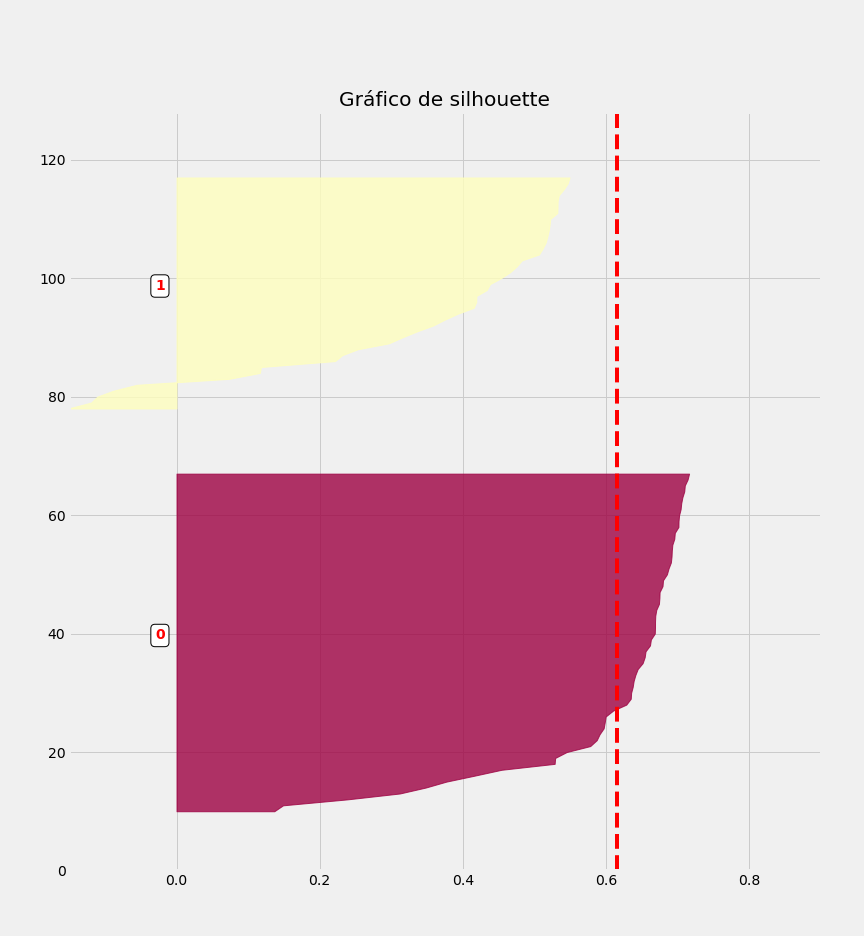
\includegraphics[width=0.8\textwidth]{CoefSil2}
%\caption{Gráfico de Silhouette recomendación caso de prueba 2 }
%\label{fig:silrdos}
%\end{figure}

\begin{table}[H]\centering
\caption{Caso de prueba 3: Resultados recomendación para el trabajo de grado Construcción de un repositorio limpio de datos para la detección de patrones de eventos eruptivos del volcán galeras con técnicas de minería de datos.}\label{tab:tablae3}
	\begin{tabularx}{\textwidth}{XXXm{3.0cm}}\toprule

Id &  \multicolumn{1}{c}{Distancia Milikowski } & \multicolumn{1}{c}{Titulo} \\ 
5268 &0.0685 &Detección automática de registros sísmicos asociados al comportamiento del volcán galeras haciendo uso de redes neuronales artificiales.  \\ 
446 & 0.1015 &Monitoreo electromagnético de volcanes.   \\ 
183 & 0.1615 &Implementación de un método fundamentado en la distribución de amplitudes para la localización de sismos asociados al movimiento de fluidos en el volcán galeras, Colombia.   \\ 
4081 &0.3012&Diseño e implementación de estación modelo de registro, trasmisión y recepción de eventos micro-sísmicos de la red sísmica de san juan de pasto. \\
4130 & 0.3286&Diseño e implementación del prototipo de una estación meteorológica automática portátil capaz de transmitir los datos mediante tecnología gsm. \\ 

 \bottomrule
	\end{tabularx}
	
\end{table}

%\begin{figure}[H]\centering
%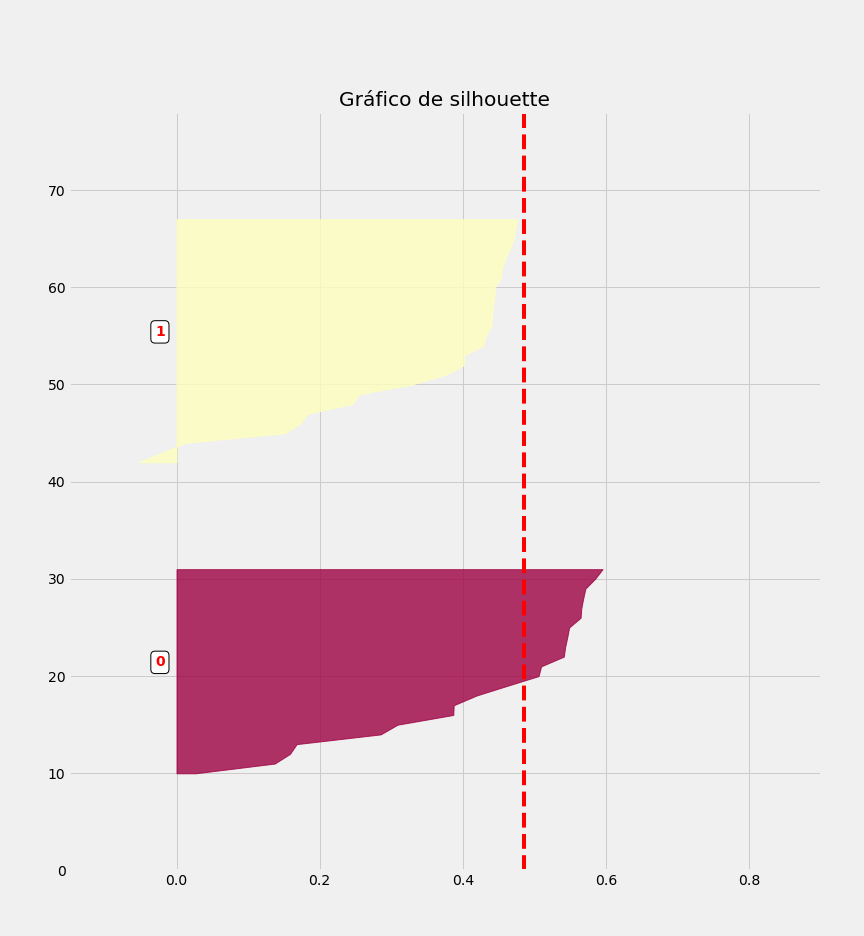
\includegraphics[width=0.8\textwidth]{CoefSil3}
%\caption{Gráfico de Silhouette recomendación caso de prueba 3 }
%\label{fig:silrtres}
%\end{figure}


%En las figura \ref{fig:silruno}, \ref{fig:silrdos} y ~\ref{fig:silrtres} se puede apreciar que los documentos relacionados propuestos por Maskanita (color rojo) están cohesionados de forma correcta a su grupo, ya que no se observan valores de silueta negativos, los valores promedio de silhouette para los 3 casos son de 0.58, 0.62 y 0.5 respectivamente; indicando  que los grupos se ajustan adecuadamente, en las ~\ref{fig:silrdos} y  ~\ref{fig:silrtres} se puede observar algunos valores de silhouette negativos en el grupo de documentos que no fueron relacionados por Maskanita (color amarillo), lo cual indica que no se cohesionan correctamente, ya que podría existir un tercer grupo o tercer dominio donde estos se agrupen adecuadamente; lo cual no es de importancia ya que la atención se centra en el grupo de documentos relacionados por el método implementado.







\chapter{Discusión }


En este capítulo se discuten y evalúan los resultados obtenidos.

\section{Comparación  de relaciones categoriales  de trabajos de grado de acuerdo a su dominio de conocimiento.}

En esta sección se evalúa las relaciones conceptuales taxonómicas o relaciones categoriales de los métodos propuestos en este trabajo. Dado que los trabajos de grado de este tipo de relaciones tienen rasgos comunes, las vinculaciones se establecen principalmente mediante mecanismos de detección de similitudes.

La medida de validación interna del agrupamiento, que se utiliza en este trabajo, consiste en determinar qué tan cohesionados están los grupos entre sí, se busca que los documentos relacionados de un mismo grupo se parezcan contextualmente más entre ellos que con los documentos de otros grupos; y por otra parte determinar qué tan separados son los documentos de un grupo con respecto a todos los documentos de otros grupos. 
Por tanto, la métrica que permite evaluar la agrupación de los dominios obtenidos es el coeficiente de Silhouette.

El coeficiente de Silhouette muestra qué documentos se encuentran completamente dentro de un grupo y cuáles han sido mal clasificados. Esta métrica tiene un rango de [-1, 1], un valor  mayor a 0 y cercano a 1 indica que el documento está lejos de los grupos vecinos, 0 indica que el documento está en o muy cerca de la frontera de decisión entre dos grupos vecinos, y valores negativos indican que el documento podría haber sido mal asignado al grupo.

\begin{table}[H]\centering
\caption{Validación Coeficiente de Silhouette algoritmo k medias para los conjuntos de datos generados }\label{tab:tablaeres}
	\begin{tabularx}{\textwidth}{XXXm{3.0cm}}\toprule

Modelo &  Coeficiente de Silhouette & K óptimo (20 –44)  \\
Doc2vec PV-DBOW & 0.36 & 32 \\
Doc2vec PV-DM &  0.34  & 27\\
Tf-idf 20000 variables & 0.04 & 38  \\
Tf-idf 10000 variables & -0.009 & 43 \\

 \bottomrule
	\end{tabularx}
\end{table}

En la tabla \ref{tab:tablaeres} se observa que el valor más alto de coeficiente de Silhouette está en los conjuntos generados por los modelos Doc2vec, por tanto  los algoritmos implementados en esta investigación se basaron en estos, particularmente en Do2vec PV-DBOW; ya que logra una mejor agrupación y separación de los dominós de conocimiento en el corpus de trabajos de grado de la universidad de Nariño.

\begin{figure}[H]\centering
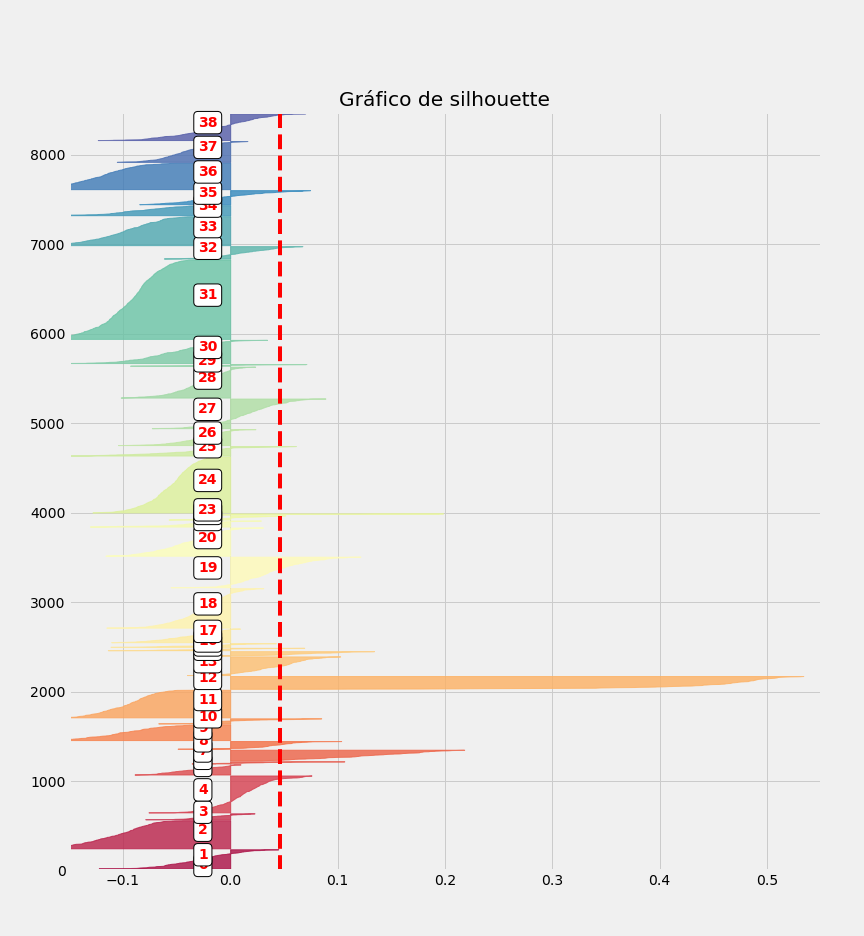
\includegraphics[width=0.8\textwidth]{CoefSilTFidf}
\caption{Gráfico de Silhouette algoritmo Kmedias con k=38 , Tf-idf 20000 variables}
\label{fig:siltfidf}
\end{figure}

En el gráfico de silhouette generado por el algoritmo Kmedias con k=38,Tf-idf 20000 variables, figura \ref{fig:siltfidf} se observa que la mayoría de los documentos del corpus fueron mal clasificados a su grupo ya que tienen un valor negativo de silhouette.

\begin{figure}[H]\centering
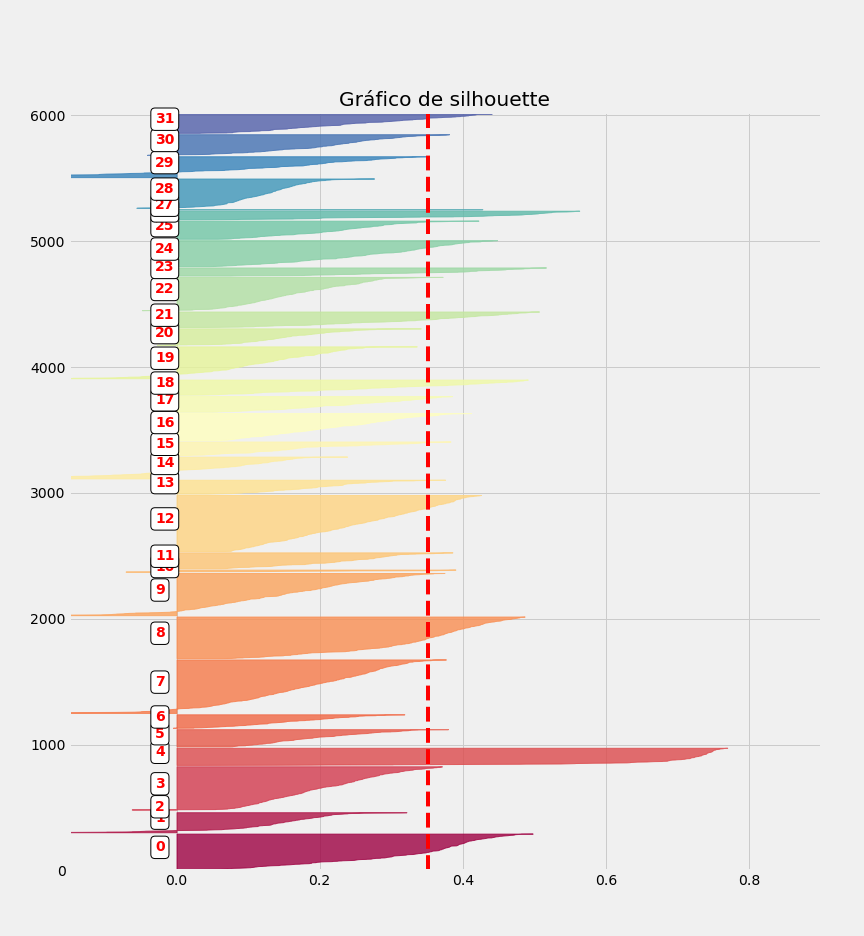
\includegraphics[width=0.8\textwidth]{CoefSilgeneral}
\caption{Gráfico de Silhouette algoritmo Kmedias con k=32 , método Doc2vec PV-DBOW}
\label{fig:sil1}
\end{figure}

 Por otro parte, en el gráfico de silhouette generado por el algoritmo Kmedias con k=32, método Doc2vec PVDBOW, figura \ref{fig:sil1} se observa que a pesar de existir documentos que quedaron mal clasificados; la gran mayoría de documentos están cohesionados de forma correcta a su respectivo grupo, Doc2vec tiene un rendimiento claramente superior a tf-idf por tanto es el método que se elige para relacionar trabajos de grado conceptualmente y generar recomendaciones.  


Contrastando con \cite{kim2019multi} lograron obtener mejores resultados ensamblando los modelos TF-IDF, IDA Y Doc2Vec , los resultados de la presente investigación de la tabla  \ref{tab:ProgramasDM} demuestran que los conjuntos estructurados con los métodos  TF-IDF  no tienen tendencia al agrupamiento por tal motivo este método quedó descartado para el repositorio de trabajos de grado.

En \cite{nandi2018bangla}  se observa que el método Doc2vec coincide en los resultados, reiterando que este tiene un mejor rendimiento y puede ser implementado en diferentes dominios de conocimiento.

 %%%%%%%%%%%%%%%%%%%%%%%%%%%%%%%%%%%%%%%%%%%%%%%%%%%%%%%%%%%%%%%%%%%%%%%%%%%%%%%%%%%%%%%%%%%%%%%%%%%%%%%%%%%%%%%%%%%%%%%%%%%%%%%%%%%%%%%%%%%%%%%%%%


%\section{Evaluación de trabajos de grado relacionados conceptualmente propuestos por Maskana.}
%
%Para la evaluación de los trabajos relacionados propuestos por el algoritmo Maskanita, se realizaron 3 casos de prueba, para los cuales se elaboró una tabla con los resultados obtenidos de las relaciones encontradas para diferentes trabajos de grado, para validar las relaciones propuestas por Maskanita se formaron dos grupos de trabajos; los que fueron relacionados por el algoritmo y los se quedaron por fuera de la frontera de decisión y no se relacionaron, para cada prueba se evalúa el coeficiente de silhouette y se valida la cohesión de los trabajos relacionados y la separación con respecto al grupo de trabajos que no se relacionaron.
%
%
%\begin{table}[H]\centering
%\caption{Caso de prueba 1: Resultados recomendación para el trabajo de grado Tariykdd: Una herramienta genérica de descubrimiento de conocimiento en bases de datos débilmente acoplada con el sgbd Postgresql.}\label{tab:tablae1}
%	\begin{tabularx}{\textwidth}{XXXm{3.0cm}}\toprule
%
%Id &  \multicolumn{1}{c}{Distancia Milikowski } & \multicolumn{1}{c}{Titulo} \\ 
%5268 &0.0006 &Pg\_KDD - Entorno Gráfico para el Sistema de Descubrimiento de 
%Conocimiento en Bases de Datos PostgresKDD.   \\ 
%446 &  0.0007 &Implantación de primitivas sql para el descubrimiento de reglas de asociación y clasificación al interior del motor del sistema gestor de bases de datos postgresql.   \\ 
%183 & 0.0033 &MATE-KDD: Una herramienta genérica para el descubrimiento.   \\ 
%4081 &0.0097&EXDACLET: Herramienta de datacleaning basada en agentes inteligentes orientadas a la web \\
%
% \bottomrule
%	\end{tabularx}
%	
%\end{table}
%
%\begin{table}[H]\centering
%\label{tab:tablae1}
%	\begin{tabularx}{\textwidth}{XXXm{3.0cm}}\toprule
%
%%Id &  \multicolumn{1}{c}{Distancia Milikowski } & \multicolumn{1}{c}{Titulo} \\ 
%4130 & 0.0363  &RASEMUS: Una herramienta para el descubrimiento de conocimiento en bases de datos con técnicas de clustering, débilmente acoplado con el sgbd postgresql. \\ 
%6975&0.1320&POLARIS: Herramienta de minería de uso para la web. \\
%6206&0.1537&GRFPOSTGRES – Herramienta gráfica para el motor de base de datos postgres.\\
%5044&0.1555&STARCUBE: Una herramienta ROLAP de análisis multidimensional para el soporte a la toma de decisiones, débilmente acoplada con el SGBD PostgreSQL. \\
% \bottomrule
%	\end{tabularx}
%	
%\end{table}
%
%\begin{figure}[H]\centering
%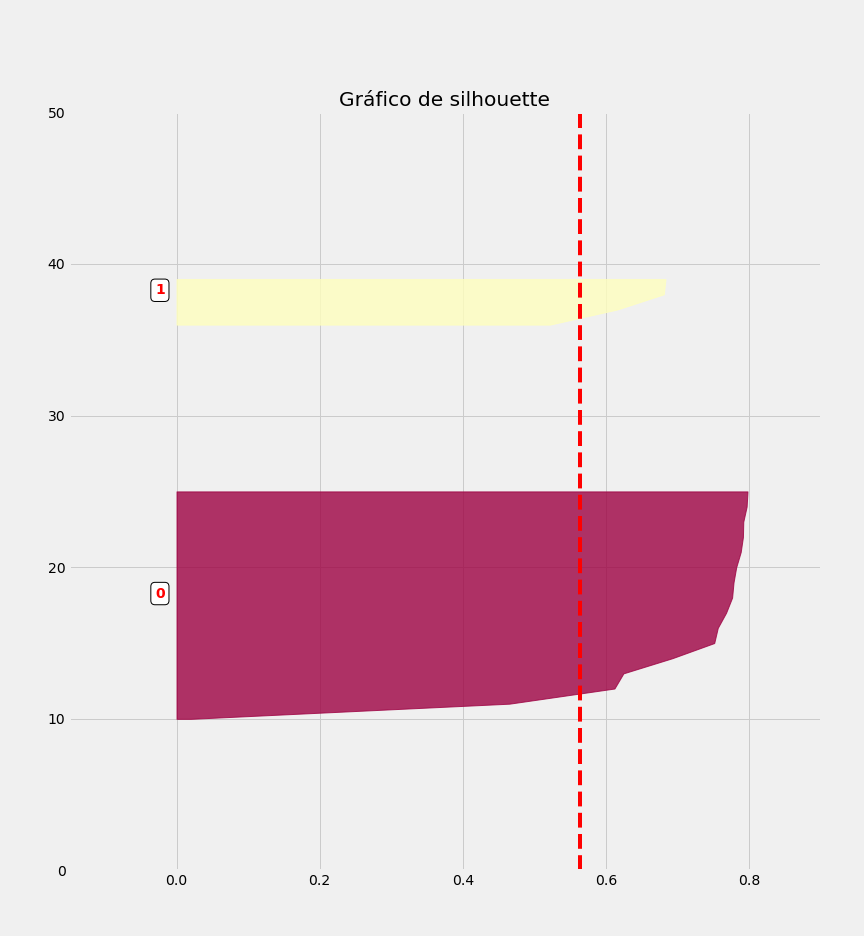
\includegraphics[width=0.8\textwidth]{CoefSil1}
%\caption{Gráfico de Silhouette recomendación caso de prueba 1 }
%\label{fig:silruno}
%\end{figure}
%
%
%
%
%\begin{table}[H]\centering
%\caption{Caso de prueba 2: Resultados recomendación para el trabajo de grado Desarrollo e implementación de un sistema de reconocimiento de comandos de voz basado en redes neuronales para la activación de dispositivos electrónicos.}\label{tab:tablae2}
%	\begin{tabularx}{\textwidth}{XXXm{3.0cm}}\toprule
%
%Id &  \multicolumn{1}{c}{Distancia Milikowski } & \multicolumn{1}{c}{Titulo} \\ 
%5268 &0.0066 &Sistema interactivo de reconocimiento de fonemas para la interpretación de voz y traducción a lengua de señas.  \\ 
%446 &  0.0067 &Implementación de redes neuronales artificiales en hardware reconfigurable.Implementación de redes neuronales artificiales en hardware reconfigurable.   \\ 
%183 & 0.0087 &Análisis de deformaciones debidas a esfuerzos, vibraciones o variaciones de temperatura en un objeto mediante metrología óptica basada en técnicas de interferometría holográfica.   \\ 
%4081 &0.0122&Diseño e implementación de un sistema que activa dispositivos electrónicos mediante señales oculares para mejorar la comunicación a personas con discapacidad motora. \\
%4130 & 0.0314  &Detección automática de registros sísmicos asociados al comportamiento del volcán galeras haciendo uso de redes. \\ 
%
% \bottomrule
%	\end{tabularx}
%	
%\end{table}
%
%
%\begin{table}[H]\centering
%\label{tab:tablae2}
%	\begin{tabularx}{\textwidth}{XXXm{3.0cm}}\toprule
%
%%Id &  \multicolumn{1}{c}{Distancia Milikowski } & \multicolumn{1}{c}{Titulo} \\ 
%6975&0.0395&Evaluar un acople colimador fibra óptica para valorar su comportamiento como medidor de intensidad luminosa. \\
%6206&0.0476&Optimización de un sistema de control para la navegación basado en el método de campo de fuerza virtual para un vehículo autónomo empleando algoritmos genéticos.\\
%5044&0.0526&Diseño e implementación de un sistema portátil de registro de señales micro-sísmicas. \\
%5044&0.0648&Identificación de aves a partir de canto característico e información contenida en bases de datos. \\
%5044&0.0786&Diseño e implementación del prototipo de un osciloscopio. \\
%
% \bottomrule
%	\end{tabularx}
%	
%\end{table}
%
%\begin{figure}[H]\centering
%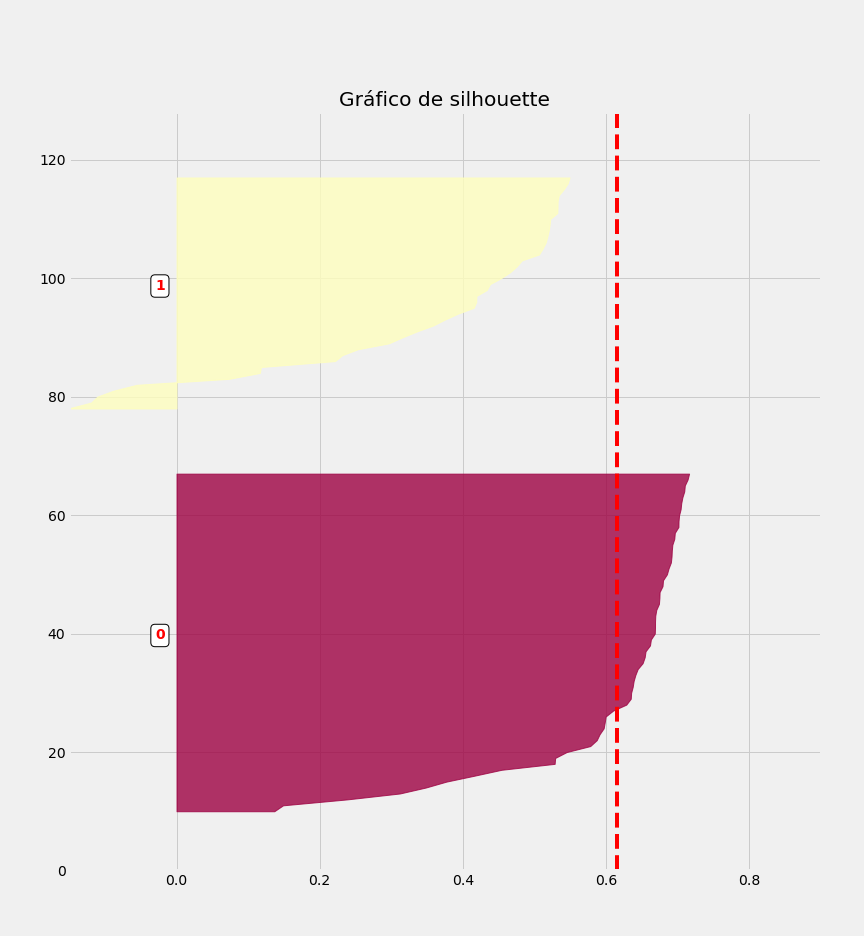
\includegraphics[width=0.8\textwidth]{CoefSil2}
%\caption{Gráfico de Silhouette recomendación caso de prueba 2 }
%\label{fig:silrdos}
%\end{figure}
%
%\begin{table}[H]\centering
%\caption{Caso de prueba 3: Resultados recomendación para el trabajo de grado Construcción de un repositorio limpio de datos para la detección de patrones de eventos eruptivos del volcán galeras con técnicas de minería de datos.}\label{tab:tablae3}
%	\begin{tabularx}{\textwidth}{XXXm{3.0cm}}\toprule
%
%Id &  \multicolumn{1}{c}{Distancia Milikowski } & \multicolumn{1}{c}{Titulo} \\ 
%5268 &0.0685 &Detección automática de registros sísmicos asociados al comportamiento del volcán galeras haciendo uso de redes neuronales artificiales.  \\ 
%446 & 0.1015 &Monitoreo electromagnético de volcanes.   \\ 
%183 & 0.1615 &Implementación de un método fundamentado en la distribución de amplitudes para la localización de sismos asociados al movimiento de fluidos en el volcán galeras, Colombia.   \\ 
%4081 &0.3012&Diseño e implementación de estación modelo de registro, trasmisión y recepción de eventos micro-sísmicos de la red sísmica de san juan de pasto. \\
%4130 & 0.3286&Diseño e implementación del prototipo de una estación meteorológica automática portátil capaz de transmitir los datos mediante tecnología gsm. \\ 
%
% \bottomrule
%	\end{tabularx}
%	
%\end{table}
%
%\begin{figure}[H]\centering
%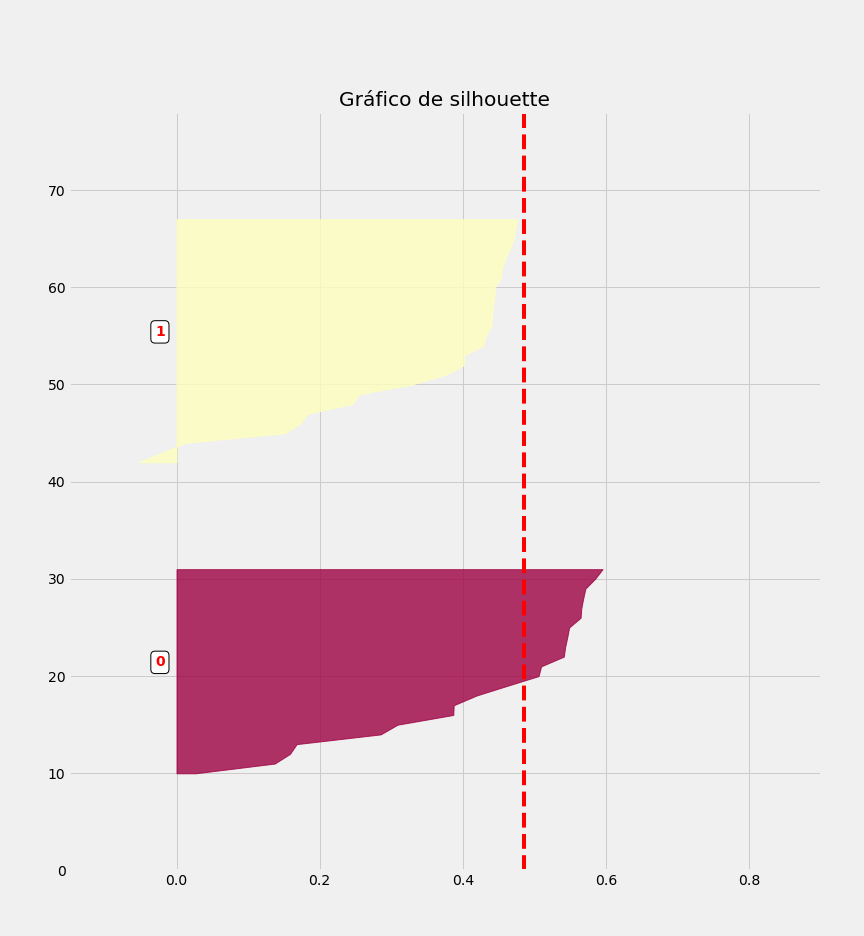
\includegraphics[width=0.8\textwidth]{CoefSil3}
%\caption{Gráfico de Silhouette recomendación caso de prueba 3 }
%\label{fig:silrtres}
%\end{figure}
%
%
%En las figura \ref{fig:silruno}, \ref{fig:silrdos} y ~\ref{fig:silrtres} se puede apreciar que los documentos relacionados propuestos por Maskanita (color rojo) están cohesionados de forma correcta a su grupo, ya que no se observan valores de silueta negativos, los valores promedio de silhouette para los 3 casos son de 0.58, 0.62 y 0.5 respectivamente; indicando  que los grupos se ajustan adecuadamente, en las ~\ref{fig:silrdos} y  ~\ref{fig:silrtres} se puede observar algunos valores de silhouette negativos en el grupo de documentos que no fueron relacionados por Maskanita (color amarillo), lo cual indica que no se cohesionan correctamente, ya que podría existir un tercer grupo o tercer dominio donde estos se agrupen adecuadamente; lo cual no es de importancia ya que la atención se centra en el grupo de documentos relacionados por el método implementado.

%\section{Interpretación de las categorías  mediante grafos conceptuales.}
%
%En esta sección se interpreta el conocimiento obtenido mediante grafos conceptuales, los cuales permiten visualizar relaciones conceptuales temáticas; organizando contextualmente el corpus de trabajos de grado; soportadas por el modelo Word2vec, estos fueron elaborados para trabajos de grado relacionados encontrados en diferentes áreas de conocimiento de cada grupo formado.
%En la figura \ref{fig:procesocinco} se observa la distribución de los diferentes documentos del repositorio; estructurados por el modelo Doc2vec con su respectivo grupo en coordenadas de las componentes principales. A continuación, se interpreta cada grupo y el dominio de conocimiento que representa.
%
%\begin{figure}[H]
%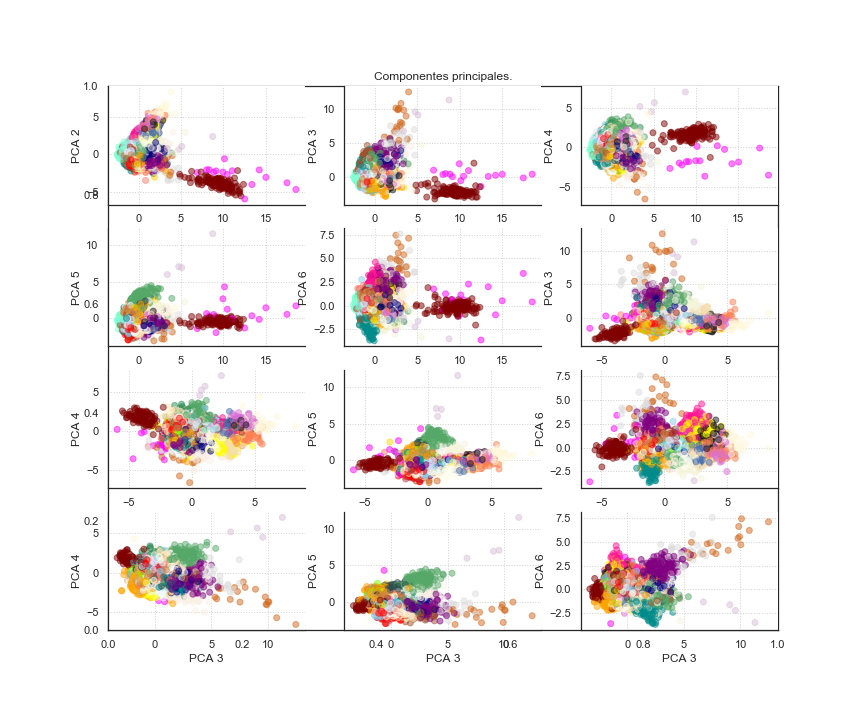
\includegraphics[width=1\textwidth]{proceso5}
%\caption{Biplot componentes principales}
%\label{fig:procesocinco}
%\end{figure}
%
%En el grupo 0 se encuentran trabajos relacionados a temáticas respectivas a los derechos humanos, derechos constitucionales, derechos laborales, derechos penales, derecho judicial, derecho administrativo, leyes y artículos constitucionales.
%En el grupo 1 se encuentran trabajos de grado relacionados a temáticas de desempleo, desigualdad social , condiciones socioeconómicas, fortalecimiento del comercio y economía. 
%En el grupo 2 se encuentran trabajos relacionados a temáticas de relaciones interfamiliares, estudios de violencia, conflictos familiares, machismo, patriarcado y problemáticas dentro del contexto sociológico como describe la figura \ref{fig:grupo14}.
%\begin{figure}[H]\centering
%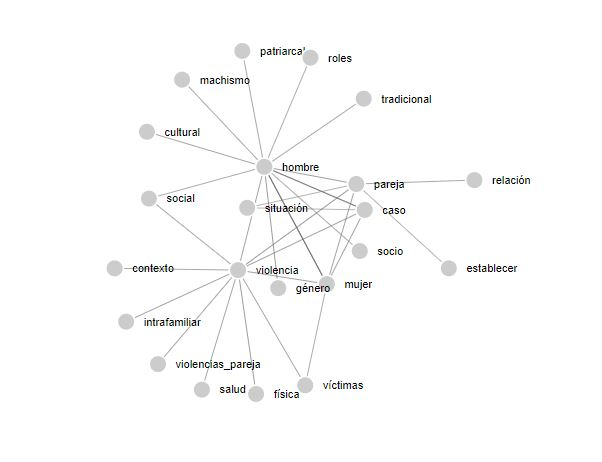
\includegraphics[width=0.8\textwidth]{grupo14}
%%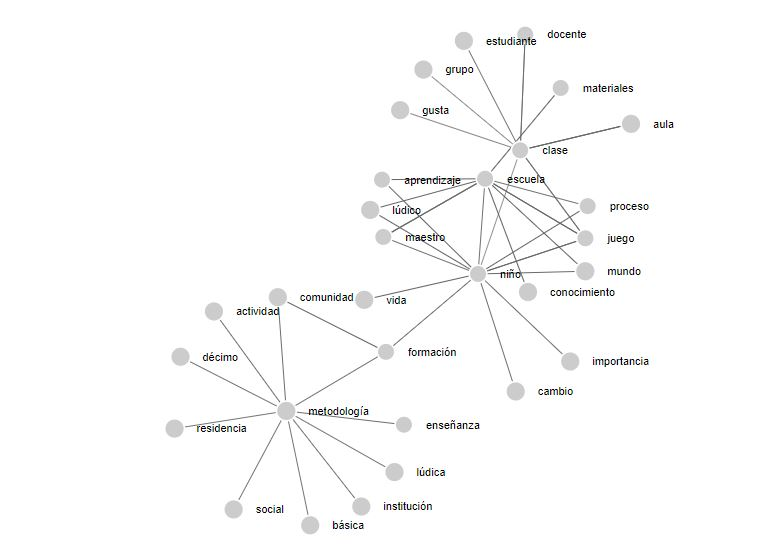
\includegraphics[width=0.8\textwidth]{grupo8}
%\caption{Grafo  relaciones temáticas grupo 2 }
%\label{fig:grupo14}
%\end{figure}
%
%%En el grupo 8 se encuentran trabajos relacionados con temáticas pedagógicas para la educación básica primaria. 
%%\begin{figure}[H]\centering
%%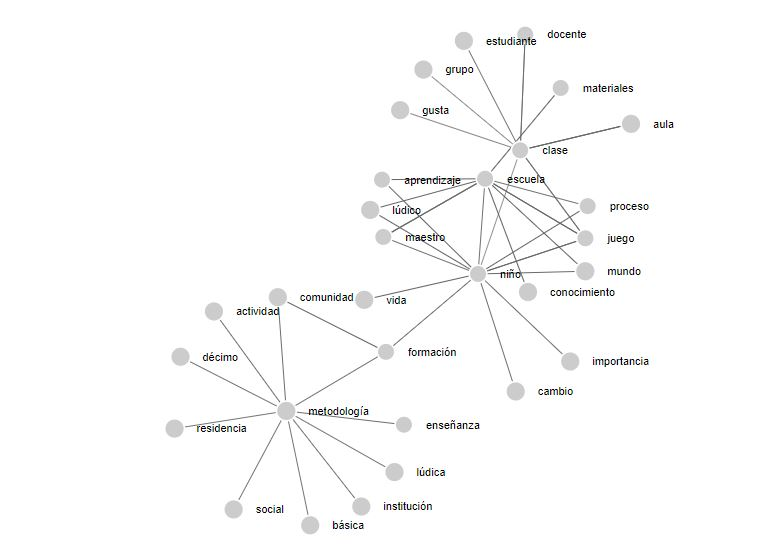
\includegraphics[width=0.8\textwidth]{grupo8}
%%\caption{Grafo  relaciones temáticas  grupo 8 }
%%\label{fig:grupo8}
%%\end{figure}
%
%%En la figura \ref{fig:grupo14} podemos observar relaciones contextuales complementarias del grupo 8 tales como: escuela, maestros , aulas de clase, estrategias y metodologías didácticas de aprendizaje basadas en lúdicas y juegos para niños estudiantes de básica  primaria.
%
%En el grupo 3 se encuentran trabajos de grado relacionados a temáticas de planeación estratégica empresarial, marketing y estudios de comercio en  organizaciones, como se puede observar en la figura \ref{fig:grupo5} .
%\begin{figure}[H]\centering
%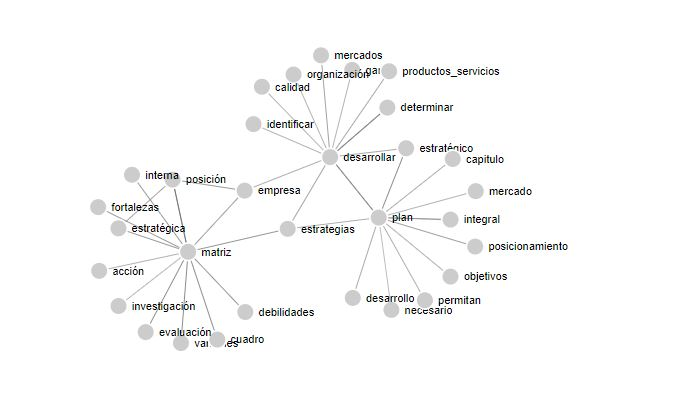
\includegraphics[width=1\textwidth]{grupo5}
%\caption{Grafo relaciones temáticas grupo 3 }
%\label{fig:grupo5}
%\end{figure}
%
%En el grupo 4 se encuentran trabajos de grado relacionados al departamento de idiomas, todos los documentos de este grupo se encuentran en idioma inglés, reprentado en la figura \ref{fig:grupo6}.
%
%\begin{figure}[H]\centering
%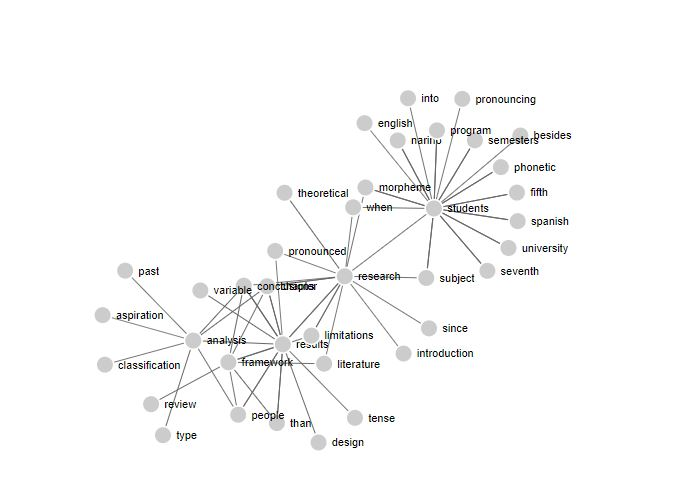
\includegraphics[width=0.8\textwidth]{grupo6}
%\caption{Grafo  relaciones temáticas grupo 4 }
%\label{fig:grupo6}
%\end{figure}
%
%En el grupo 5 se encuentran trabajos de grados vinculados a la facultad de ciencias exactas, específicamente al programa de Biología, evaluando diferentes tratamientos para encontrar diferencias estadísticamente significativas entre estos y así mejorar el crecimiento y producción de especies. %%
%
%En el grupo 6 se encuentran trabajos relacionados al estudio de modelamiento de fluidos.
%
%En el grupo 7 se encuentran trabajos de grado relacionados a temas de cultura, carnavales, historia y desarrollo social.
%\begin{figure}[H]\centering
%\includegraphics[width=0.8\textwidth]{grafocul0}
%\caption{Grafo  relaciones temáticas grupo 7 }
%\label{fig:grafoculcero}
%\end{figure}
%
%
%
%La figuera \ref{fig:grafoculcero}  se muestra el grafo  conceptual  de los trabajos de grado clasificados en el grupo 7, donde se observa conceptos relacionados referentes al carnaval de negros y blancos, cultura, artes , maestros y artesanos.
%
%En el grupo 8 se encuentran trabajos relacionados a construcción, desarrollo, gestión de calidad y auditoría de obras civiles.
%
%En el grupo 9 se encuentran trabajos de grado relacionados con temáticas pedagógicas de aprendizaje   y estrategias lúdicas de aprendizaje  para estudiantes.
%
%En el grupo 10 se encuentran trabajos de grado relacionados específicamente a ingeniería de software, lenguaje unificado de modelado UML, desarrollo y construcción de módulos y sistemas de información a la medida.
%
%En el grupo 11 se encuentran trabajos relacionados a telemática, microcontroladores, reconocimiento de imágenes, redes neuronales ,  espectro electromagnético,  series temporales,  aplicaciones en vulcanología y sismología. 
%
%En el grupo 12 se encuentran trabajos de grado vinculados al programa de ingeniería agroindustrial referentes a temáticas de desarrollo, comercialización, industrialización, estudios de oferta y demanda de productos agropecuarios.
%
%En el grupo 13 se encuentran trabajos de grado en temáticas de ordenamiento territorial, desarrollo sostenible y seguridad social.  %%%%%
%
%En el grupo 14 se encuentran trabajos de grado relacionados con proyectos referentes a entornos y herramientas virtuales de aprendizaje.
%
%En el grupo 15 se encuentran trabajos de grado vinculados a esquemas de seguridad, salud ocupacional en la industria y riesgos laborales como se describe en la figura \ref{fig:grupo22}
%
%
%\begin{figure}[H]\centering
%\includegraphics[width=0.8\textwidth]{grupo22}
%\caption{Grafo  relaciones temáticas grupo 15}
%\label{fig:grupo22}
%\end{figure}
%
%
%En el grupo 16 se encuentran trabajos de grado relacionados a cultivos, recursos hídricos  , plantas, especies y temáticas agroforestales como se observa en la figura \ref{fig:grupo1especies}.
%\begin{figure}[H]\centering
%\includegraphics[width=1\textwidth]{grupo1especies}
%\caption{Grafo relaciones temáticas grupo 16 }
%\label{fig:grupo1especies}
%\end{figure}
%
%El grupo 17 contiene tópicos relacionados con bacterias, microorganismos, compuestos antioxidantes, proteínas y aminoácidos como se describe en la figura \ref{fig:grupo25}.
%\begin{figure}[H]\centering
%\includegraphics[width=0.8\textwidth]{grupo25}
%\caption{Grafo  relaciones temáticas grupo 17}
%\label{fig:grupo25}
%\end{figure}
%
%En el grupo 18 se encuentran trabajos relacionados con temáticas temáticas afines a administración, economía y finanza empresarial.
%
%En el grupo 19 se encuentran trabajos relacionados a temáticas sociales, desarrollo humano sostenible, desarrollo económico social, derecho internacional humanitario y políticas comunitarias.
%
%En el grupo 20 se encuentran trabajos de grado de la facultad de artes, referentes a temáticas culturales, artesanías e  historia del arte.
%
%En el grupo 21 se encuentran trabajos relacionados a la facultad de ciencias económicas y administrativas los cuales involucran temáticas de comercio exterior, aduanas, exportaciones, impuestos, empresas, fiscalización y estudios de mercados.
%
%
%En el grupo 22 se encuentran trabajos de grado relacionados con planes de ordenamiento  territorial   y ecoturismo tal como se observa en la figura \ref{fig:ordenaminetoimg}.
%
%
%\begin{figure}[H]\centering
%\includegraphics[width=1\textwidth]{ordenaminetoimg}
%\caption{Grafo relaciones temáticas grupo 22 }
%\label{fig:ordenaminetoimg}
%\end{figure}
%
%En el grupo 23 se encuentran trabajos de grado de la facultad de ciencias agrícolas, específicamente del programa de ingeniería agronómica, relacionando temáticas referentes a estudios de variedades de especies de granos, tubérculos, plantas y técnicas de comparación de diferentes tratamientos agronómicos mediante pruebas de Tukey y validaciones estadísticas
%como se representa en la figura \ref{fig:grupo25}.
%\begin{figure}[H]\centering
%\includegraphics[width=0.8\textwidth]{grupo28}
%\caption{Grafo  relaciones temáticas grupo 23}
%\label{fig:grupo25}
%\end{figure}
%
%
%En el grupo 24 se encuentran trabajos relacionados con medicina veterinaria, en la figura \ref{fig:grupo7} se aprecia relaciones entre enfermedades causadas por las bacterias babesia y  anaplasma en equinos.
%
%\begin{figure}[H]\centering
%\includegraphics[width=0.8\textwidth]{grupo7}
%\caption{Grafo  relaciones temáticas grupo 24 }
%\label{fig:grupo7}
%\end{figure}
%
%En el grupo 25 se encuentran trabajos de grado relacionados con proyectos de priorización de áreas ambientales, caracterización de sistemas agroforestales, investigación de especies y reservas naturales.  %%
%
%En el grupo 26 se encuentran trabajos de grado relacionados con música.
%
%En el grupo 27 se encuentran trabajos relacionados con temáticas pedagógicas para la educación. 
%\begin{figure}[H]\centering
%\includegraphics[width=0.8\textwidth]{grupo8}
%\caption{Grafo  relaciones temáticas grupo 27 }
%\label{fig:grupo8}
%\end{figure}
%
%En la figura \ref{fig:grupo8} podemos observar relaciones contextuales complementarias del grupo 27 tales como: escuela, maestros , aulas de clase, estrategias y metodologías didácticas de aprendizaje basadas en lúdicas y juegos para niños estudiantes de básica  primaria.
%
%En el grupo 28 se encuentran trabajos de grado relacionados al programa de administración empresas, referentes a estudios del clima organizacional, talento humano, selección de personal, control interno y procesos de gestión y calidad en las empresas.
%
%En el grupo 29 se encuentran trabajos de grado del programa de Psicología, relacionados con factores de riesgo en adolencetes causantes de suicidio, identificación de ideas suicidas como se describe en la figura \ref{fig:grupo14}.
%\begin{figure}[H]\centering
%\includegraphics[width=0.8\textwidth]{grupo19}
%\caption{Grafo  relaciones temáticas grupo 29 }
%\label{fig:grupo19}
%\end{figure}
%
%En el grupo 30 se encuentran trabajos relacionados al programa de ingeniería de sistemas, particularmente al área de descubrimiento de conocimiento en base de datos, desarrollo de herramientas bajo el gestor Postgresql, algoritmos de minería de datos, clasificación, agrupación, reglas de asociación y temáticas de software y manejo de información.
%
%\begin{figure}[H]\centering
%\includegraphics[width=0.8\textwidth]{grafotarykdd}
%\caption{Grafo  relaciones temáticas grupo 30 }
%\label{fig:tarygradfo}
%\end{figure}
%
%En las figuras \ref{fig:tarygradfo}  se muestra el grafo conceptual generado por el modelo Word2vec de los trabajos de grado respectivos al  grupo 30. Donde se pueden establecer vínculos entre conceptos dentro de minería de datos, descubrimiento de conocimiento, algoritmos de clasificación y asociación tales como equipasso, fpgrowth, entrenamiento de  árboles  de decisión, a priori e itemsets frecuentes.
%
%En el grupo 31 se encuentran trabajos de grado relacionados con las ciencias pecuarias, producción acuícola y comparación de dietas en cultivos de peces.


\section{Comparación  de los dominios de conocimiento entrenados.}

Para saber que modelo distingue mejor las áreas de conocimiento de los documentos  estructurados por el método  Doc2vec, se evalúa y compara cada clasificador entrenado.
  Se utilizaron las métricas de accuracy (exactitud) y f1 para los conjuntos de entrenamiento (70\%),   testing (30\%) y el método de validación cruzada (k fold=5). La accuracy expresa la cantidad de casos correctamente clasificados sobre el total, y F1 (F-Score o medida-F) la medida de precisión que tiene un test, ponderando la precisión y la exhaustividad, la medida f1 se calculó con la fórmula Macro-averaged F-Measure explicada  en  \cite{ozgur2005text}.

\begin{figure}[H]
\includegraphics[width=0.5\textwidth ,height=350]{clasificadoresA}
\includegraphics[width=0.5\textwidth ,height=350]{clasificadoresF1}
\caption{Comparativa de los clasificadores entrenados }
\label{fig:clasificadoresA}
\end{figure}

En la figura \ref{fig:clasificadoresA} se aprecia que los modelos sufren un ligero sobreajuste en el conjunto de entrenamiento, el modelo RandomForestes el más sobre ajustado, ya que baja notoriamente su performance en el conjunto de testing y el método de validación cruzada.
El único clasificador que obtiene resultados notablemente más bajos es el árbol de decisión , mientras que los otros obtienen puntajes por encima del 80\%.
Los mejores modelos en términos de Accuracy y F1 en los conjuntos de validación son Xgboost y Regresión logística; a pesar de que el modelo Xgboost está un poco más sobre ajustado al conjunto de entrenamiento, es el que obtuvo mejores resultados en test, por tanto es el modelo utilizado  en el algoritmo \ref{alg:maskanita1} y para la clasificación  de los nuevos documentos que ingresen al repositorio. En \cite{seyfiouglu2017hierarchical} se obtiene una precisión general del 92,5\% utilizando el modelo XGBOOST bajo un corpus estructurado con Doc2vec para una clasificación binaria, para la clasificación de 12 categorías obtuvieron una precisión general del 71,16\%, la diferencia con respecto a la precisión obtenida en esta investigación puede darse por los dominios de conocimiento entre repositorios y también los métodos de obtención de las categorías a entrenar; ya que en este  método propuesto se obtuvo la clase a partir del agrupamiento validado con el coeficiente de silhouette, por tanto la adopción de técnicas complejas no siempre garantizan el logro de obtener mejores resultados y  pueden variar de acuerdo a los repositorios textuales que se pretendan investigar.

\begin{figure}[H]\centering
\includegraphics[width=0.8\textwidth]{matrixbost}
\caption{Matriz de confusión modelo Xgboost para el conjunto de testing}
\label{fig:mconf}
\end{figure}

En la figura \ref{fig:mconf} se muestra la matriz de confusión en testing para el mejor modelo de Xgboost. El porcentaje de casos correctamente clasificados es de 90\%; los casos mal clasificados con un desvío de clase entre los grupos 2 y 27 se debe a que existe correlación entre los dominios de conocimiento, el algoritmo  \ref{alg:maskanita1}  toma las probabilidades asignadas por el modelo Xgboost y busca documentos similares entre los grupos con más alta probabilidad.

Se reproduce un caso a modo de ejemplo del algoritmo \ref{alg:maskanita1}. Se trata de un nuevo trabajo que contenga ''perceptrones multicapa backpropagation''. El algoritmo predice que este tema se relaciona con el grupo 11 con una probabilidad de 99\% y los documentos más similares dentro del grupo son: 
''Detección automática de registros sísmicos asociados al comportamiento del volcán galeras haciendo uso de redes neuronales artificiales'' con una similitud de 0.84 y ''Diseño e implementación de un sistema clasificador prototipo de granos de café por tamaño y color'' con una similitud de 0.82.






% \chapter{ALGORITMO FP-FLOCK}

En el algoritmo propuesto por \cite{VieiraT13}, en la primera parte del algoritmo se encuentra el total de discos con los 
objetos móviles que están juntos, se eliminan discos que no cumplan $\mu$, este proceso genera que se encuentren varios de
 los discos solapados, para ello, por último, se realiza una limpieza de los discos solapados haciendo iteraciones en los discos
 encontrados y dejando únicamente aquellos discos con mayor número de miembros denominados discos máximos, este proceso de
 limpieza de los discos solapados hace que el costo computacional sea muy alto debido a la cantidad de iteraciones. En la 
segunda parte, el algoritmo realiza un proceso de combinación para el descubrimiento de flocks en el cual si el $\varepsilon$ aumenta
 el algoritmo puede llegar a colapsar. Este algoritmo separa los flocks de acuerdo al parámetro $\delta$ en procura de limitar
 el número de discos a comparar, esto dificulta la interpretación de resultados ya que es necesario de un análisis adicional 
para encontrar los flocks más largos a partir de aquellos con una duración fija.

Para el algoritmo propuesto por \cite{romero2011mining}, ya que usa la primera parte del algoritmo en \cite{VieiraT13}, tiene 
el mismo problema de los discos solapados. Ya en la segunda parte, al tratar el proceso de combinación es mucho más
eficiente ya que utiliza un enfoque basado en técnicas de patrones frecuentes, aunque con la desventaja que el proceso se 
realiza en una ventana fija  de tiempo  lo que le impide reportar patrones en tiempo real. 

La alternativa propuesta resuelve los problemas que poseen los algoritmos anteriores utilizando patrones frecuentes, se proponen 
el algoritmo llamado FP-Flock con dos variaciones, uno fuera de línea y otro en tiempo real.


\section{FP-FLOCKOFFLINE}

En la primera parte se hace el cálculo de los discos máximos, para lo cual se tomó como base el algoritmo 1 propuesto
 por \cite{VieiraT13} al cual se le hicieron modificaciones para hacer una limpieza de los discos solapados usando 
patrones frecuentes de minería. Puntualmente, se usó el algoritmo LCM \cite{uno2005lcm}. El pseudo-código de la primera
 parte del algoritmo es presentado en Algoritmo~\ref{alg:maximalDisks}. 

\begin{algorithm}
    \renewcommand{\algorithmicrequire}{\textbf{Input:}}
    \renewcommand{\algorithmicensure}{\textbf{Output:}}
    \renewcommand{\algorithmicprint}{\textbf{break}}
  \caption{Computing maximal disks.}
  \label{alg:maximalDisks}
  \algsetup{indent=2em}
  \footnotesize
  \begin{algorithmic}[1]
\REQUIRE {set of points $T[t_i]$ for timestamp $t_i$} 
\ENSURE {sets of maximal disks $C$}
\STATE $C \leftarrow \emptyset$
\STATE Index.Build($T[t_i],\varepsilon)$ \COMMENT{call Algorithm 1 in \cite{VieiraT13}}
\FOR {each non-empty cell $g_{x,y} \in$ Index}
  \STATE {$L_r \leftarrow g_x,_y$} 
  \STATE {$L_s \leftarrow [g_{x-1,y-1}... g_{x+1,y+1}]$}
  \IF {$|L_s| \geq \mu$}
    \FOR {each $l_r \in L_r$}
      \STATE {$H \leftarrow Range(l_r, \varepsilon), |H| \geq \mu, d(l_r,l_s) \leq \varepsilon, l_s \in L_s $}
      \FOR {each $l_j \in H$}
	\IF{ $\{l_r, l_j\}$ not yet computed}
	  \STATE {compute left disk $\{c\}$ defined by ${l_r, l_j}$ and diameter $\varepsilon$}
	  \STATE {D $\leftarrow$ points $\in c$ }
	\ENDIF
      \ENDFOR
    \ENDFOR
  \ENDIF
  \STATE $min\_sup \leftarrow 1$ 
  \STATE {C $\leftarrow$ call $LCM\_max(D, min\_sup)$  \COMMENT{call LCM Algorithm \cite{uno2005lcm}}}
\ENDFOR
\end{algorithmic}
\end{algorithm}

El algoritmo fuera de línea, se construyó usando el pseudo-código propuesto en \cite{turdu2014}, pero utilizando el algoritmo descrito anteriormente.

\section{FP-FLOCKONLINE}

El algoritmo en tiempo real, hace modificaciones al algoritmo propuesto en \cite{turdu2014},
este algoritmo en su primera parte usa el Algoritmo~\ref{alg:maximalDisks}, para solucionar el problema de los discos solapados.
En su segunda parte, se va liberando memoria en cada transacción, teniendo en cuenta las trayectorias que en ese 
instante de tiempo tuvieron un corte. En este algoritmo por cada intervalo de tiempo se realiza un llamado al 
algoritmo LCM propuesto por \cite{uno2005lcm} con el objetivo de reportar los patrones obtenidos hasta el momento.

El pseudo-código  del algoritmo en tiempo real es presentado en Algoritmo~\ref{alg:framework2}


\begin{algorithm}
    \renewcommand{\algorithmicrequire}{\textbf{Input:}}
    \renewcommand{\algorithmicensure}{\textbf{Output:}}
    \renewcommand{\algorithmicprint}{\textbf{break}}
  \caption{FP-FlockOnline: Frequent pattern flock  online.}

  \label{alg:framework2}

  \algsetup{indent=2em}

  \footnotesize

  \begin{algorithmic}[1]

\REQUIRE parameters $\mu$, $\varepsilon$ and $\delta$,
set of points $T$ 

\ENSURE flock patterns $F$
  \FOR{each new time instance $t_i \in T$}
    \STATE $C \leftarrow$ call $Index.Disks(T[t_i])$ \COMMENT{call Algorithm 1 in this paper}    
    \FOR{each $c_i \in C$}
      \STATE $P \leftarrow c_i.points$ 
      \FOR{each $p_i \in P$}
	  \STATE $c_i.time \leftarrow t_i$
	  \STATE $D[p_i] \leftarrow $ add $c_i.id$
      \ENDFOR
      \FOR {each $p_i \in P$}
	\IF {$D[p_i$] not was updated}
	    \STATE delete $D[p_i]$
	  \ENDIF
      \ENDFOR
    \ENDFOR
  \STATE $min\_sup \leftarrow \mu$
  \STATE $M \leftarrow$ call $LCM\_max(D,min\_sup)$ \COMMENT{call LCM Algorithm \cite{uno2005lcm}}
  \FOR{ each $max\_pattern \in M$}
  \STATE $id_0 \leftarrow max\_pattern[0]$
  \STATE $c_0 \leftarrow C[id_0]$
  \STATE $u \leftarrow c_0.points$
  \STATE $u.t_{start} \leftarrow c_0.time$
  \STATE $n \leftarrow max\_pattern.size$ 
  \FOR{$i=1$ \TO $n$}
	\STATE $id_i \leftarrow max\_pattern[i]$
	\STATE $c_i \leftarrow C[id_i]$
	\IF{$c_i.time = c_{i-1}.time + 1$} 
	  \STATE $u \leftarrow u \cap c_i.points$
	  \STATE $u.t_{end} \leftarrow c_i.time$
	\ELSE
	  \IF{$u.t_{end} - u.t_{start} > \delta$ \AND $u \notin F$}
		\STATE $F \leftarrow$ add $u$
		\STATE $u.t_{start} \leftarrow c_i.time$
	  \ENDIF
	\ENDIF
  \ENDFOR
  \IF{$u.t_{end} - u.t_{start} > \delta$ \AND $u \notin F$}
	\STATE $F \leftarrow$ add $u$
  \ENDIF
\ENDFOR
\ENDFOR

\end{algorithmic}

\end{algorithm}

\section{VALIDACIÓN}
 
Para poder validar la correcta implementación de los algoritmos se realizó el mismo proceso de  
validación mencionado en el capítulo anterior, con la implementación de BFE y LCMFlock, posterior a 
ello se realizó un proceso de validación visual.  

Para realizar una validación visual se utilizó el conjunto de datos de Oldenburg disponible en \cite{Brin:2010:Online}, el cual proporciona un conjunto de ejemplos y 
recursos que pueden ser utilizados en la demostración en línea o 
versión descargable del generador. Para empezar, se utilizó un conjunto de datos relativamente pequeña posición de 1.000 objetos en movimiento 
al azar en la ciudad alemana de Oldenburg. Los datos de la red (bordes y nodos) están disponibles en el sitio web. La simulación de datos recoge la latitud y longitud de los puntos generados durante 140 intervalos 
de tiempo. El número total de ubicaciones almacenadas es 57.016 puntos. Con este conjunto se construyeron mapas con las representaciones lineales de 
los flocks resultantes como lo muestra la tabla~\ref{tab:validacionOldenburg} con las cuatro implementaciones.
En la figura~\ref{fig:validation} se muestran los flocks obtenidos con los parámetros $\varepsilon$=300, $\mu$=3 y $\delta$=3 sobre el conjunto Oldenburg.
Estos mapas se los comparó usando un 
módulo que implementa la similitud estructural métrica de imagen (SSIM) 
\cite{Zhou2004}. Los resultados de la comparación muestran que todos los mapas son 
idénticos, y por lo tanto, los mismos flocks son reportados por los diferentes 
algoritmos.


\begin{table*}
\caption{Número de flocks generados por los algoritmos en el conjunto de Oldenburg $\mu$=3, $\delta$=3}
\label{tab:validacionOldenburg}
\centering
\begin{tabular}{c c r r c}
\toprule
$\varepsilon(m)$& BFE & LCM & FP-FlockOnline & FP-FlockOffline \\  

\midrule
50 & 131 & 27 & 150 & 27 \\
100 & 639 & 109 & 663 & 109 \\
150 & 1135 & 247 & 1226 & 247 \\
200 & 2755 & 523 & 2683 & 523 \\
250 & 5423 & 1150 & 6877 & 1150 \\
300 & 11196 & 2365 & 16671 & 2365 \\
\bottomrule
\end{tabular}\par
\bigskip
Fuente: Esta investigación.
\end{table*}


\begin{figure}
  \centering
  \subfigure[BFE]{\includegraphics[scale=0.3]{pictures/bfe.pdf}}
  \subfigure[LCMFlock]{\includegraphics[scale=0.3]{pictures/lcm.pdf}}
  \subfigure[FP-FlockOnline]{\includegraphics[scale=0.3]{pictures/fpflockOnline.pdf}}
  \subfigure[FP-FlockOffline]{\includegraphics[scale=0.3]{pictures/fpflockOffline.pdf}}
  
  \caption{Visualización Oldenburg}
  \label{fig:validation}
\end{figure}

% \chapter{EXPERIMENTACIÓN COMPUTACIONAL}

Los resultados fueron producidos usando conjuntos de datos sintéticos y reales 
en una máquina
Dell OPTIPLEX 7010 con procesador Intel\textregistered Core\texttrademark  
i7-3770 CPU de 3.40GHz x 8,
16 GB de RAM y 1TB 7200 RPM de Disco Duro, corriendo el Sistema Operativo Debian con linux 3.2. Para 
todos los casos se usaron
los algoritmos implementados en Python, versión 3.

\section{SAN JOAQUIN}

Un grupo de conjuntos de datos sintéticos fueron creados usando un modelo para 
la generación de objetos en movimiento, como se describe en 
\cite{brinkhoff2002framework}.
Dos conjuntos de datos sintéticos fueron creados usando la red de San Joaquín 
proporcionada en el sitio web del generador \cite{Brin:2010:Online}.
El primer conjunto de datos recoge 992140 lugares simulados para 25.000 objetos 
en movimiento durante 60 instantes de tiempo. El segundo recoge 50.000 
trayectorias a partir de 2.014.346 de puntos durante 55 instantes de tiempo. La 
tabla~\ref{tab:datasets}, resume la información principal. Las 
figuras~\ref{fig:SJ25K60} y~\ref{fig:SJ50K55} muestran los tiempos de desempeño 
para estos dos casos de estudio, los parámetros adicionales fueron $\mu$=5, 
$\delta$=3 y  $\mu$=9, $\delta$=3, respectivamente.


\begin{table*}
\caption{Conjunto de datos}
\label{tab:datasets}
\centering
\begin{tabular}{c c r r c}
\toprule
\multirow{2}{*}{Dataset}& \multirow{2}{*}{Red}& \multicolumn{1}{c}{Número de}& 
Número de  & Duración promedio\\
                        &                         & trayectorias & 
\multicolumn{1}{c}{puntos} & de la trayectoria\\
\midrule
SJ25KT60  & San Joaquin & 25000 & 992140  & 40\\
SJ50KT55  & San Joaquin & 50000 & 2014346 & 37\\
TAPAS Cologne  & Cologne, Alemania & 88668 & 3403463 & 38\\
Beijing\_Original   & Beijing, China   & 21573 & 1411846& 65\\
Beijing\_Alternativo   & Beijing, China   & 18700 & 815657 & 43\\
\bottomrule
\end{tabular}\par
\bigskip
\end{table*}

\begin{figure*}
  \centering
  \subfigure[BFE, LCMFlock, FPFlock]{\label{SJ25KT60A} 
\includegraphics[scale=0.55]{pictures/SJ25KT60.pdf}}
  \subfigure[LCMFlock, 
FPFlock]{\label{SJ25KT60B}\includegraphics[scale=0.55]{pictures/SJ25KT60_B.pdf}}
  \caption{Caso de Prueba: SJ25KT60. (a) BFE, LCMFlock, FPFlock (b) LCMFlock, FPFlock}
  \label{fig:SJ25K60}
\end{figure*}

\begin{figure*}
  \centering
  \subfigure[BFE, LCMFlock, FP-Flock]{\label{SJ50K55A} 
\includegraphics[scale=0.55]{pictures/SJ50KT55.pdf}}
  \subfigure[LCMFlock, FP-Flock]{\label{SJ50K55B} 
\includegraphics[scale=0.55]{pictures/SJ50KT55_B.pdf}}
  \caption{Caso de Prueba: SJ50KT55. (a) BFE, LCMFlock, FP-Flock (b) LCMFlock, FP-Flock}
  \label{fig:SJ50K55}
\end{figure*}

\section{TAPAS COLOGNE}

Este conjunto de datos sintético se preparó utilizando el escenario TAPAS 
Cologne \cite{varschen2006mikroskopische}
en SUMO \cite{krajzewicz2002sumo}, un reconocido simulador de tráfico para la 
movilidad urbana. El escenario de simulación 
TAPAS Cologne, describe el tráfico dentro de la ciudad de Colonia (Alemania) 
durante un día entero. La principal ventaja de 
este conjunto de datos es que sus trayectorias no se generan aleatoriamente. Los 
datos de la demanda original, se deriva de TAPAS, 
un sistema que calcula la tendencia de movilidad para una población con base en 
la información sobre los hábitos de viaje 
de los alemanes y en la información sobre la infraestructura de la zona en que 
viven \cite{MiD2002}. El conjunto de datos original 
es enorme por lo que sólo está disponible al público la versión de 2 horas 
\cite{TAPASCologne}. Debido a las restricciones de memoria,
se podaron las trayectorias más cortas que 20 minutos. El último conjunto de 
datos recoge 88.668 trayectorias y más 
de 3,4 millones de puntos. La tabla~\ref{tab:datasets}, describe los detalles 
sobre el conjunto de datos. Las figura~\ref{fig:Tapas} muestra los tiempos de 
desempeño para este caso de estudio. Los parámetros adicionales fueron $\mu$=10, 
$\delta$=5.

\begin{figure*}
  \centering
  \subfigure[BFE, LCMFlock, FP-Flock]{\label{tapasA} 
\includegraphics[scale=0.55]{pictures/Cologne.pdf}}
  \subfigure[LCMFlock, FP-Flock]{\label{tapasB} 
\includegraphics[scale=0.55]{pictures/Cologne_B.pdf}}  
  \caption{Caso de Prueba: Tapas Cologne. (a) BFE, LCMFlock, FP-Flock (b) LCMFlock, FP-Flock}
  \label{fig:Tapas}
\end{figure*}

\section{MOVIMIENTO DE PEATONES EN BEIJING}

Este conjunto de datos reales recopila información de movimiento de un grupo de 
personas en toda
el área metropolitana de Beijing, China\cite{GeoLife}. El conjunto de datos se 
recogió durante el proyecto Geolife por 165 usuarios anónimos en un período de 
dos años entre abril de 2007 y agosto de 2009. Las ubicaciones fueron grabadas 
por diferentes dispositivos GPS o teléfonos inteligentes y la mayoría de ellos 
presentan una frecuencia de muestreo alta. 
La región alrededor del quinto anillo vial en el área metropolitana de Beijing 
mostró la 
mayor concentración de trayectorias. Esto fue usado para generar un conjunto de 
datos de muestra. Cada trayectoria 
fue interpolada por minuto (un punto por minuto) y saltos de 20 minutos o más 
sin señal se utilizaron para marcar una nueva trayectoria. Por último, el 
conjunto de datos recoge más 
de 1,4 millones de puntos y 21.573 trayectorias. Sin embargo, como este conjunto 
de datos tuvo poca cantidad de
entidades en movimiento (165 usuarios) en una ventana de tiempo de más de 2 
años, no existieron muchas trayectorias ocurriendo al mismo tiempo. Para probar
la escalabilidad de los algoritmos, se decidió crear un conjunto de datos alternativo basado en las 
trayectorias reales, pero forzando para que todas ellas comiencen al mismo 
tiempo. Una 
vez más, por las limitaciones de memoria, las trayectorias más cortas que 10 
minutos y más largas que 3 horas se podaron. El conjunto de datos alternativo 
almacenó 815.657 
ubicaciones y 18.700 trayectorias. La tabla~\ref{tab:datasets} resume los 
detalles para ambos conjuntos de datos. Las figuras~\ref{fig:BeijingOr} 
y~\ref{fig:BeijingAl} muestran los tiempos de desempeño para estos dos casos de 
estudio, los parámetros adicionales fueron $\mu$=3, $\delta$=3 y  $\mu$=5, 
$\delta$=5 respectivamente.


\begin{figure}
  \centering
  \includegraphics[scale=0.55]{pictures/Beijing_Original.pdf}
  \caption{Caso de Prueba: Beijing Original}
  \label{fig:BeijingOr}
\end{figure}

\begin{figure*}
  \centering
  \subfigure[BFE, LCMFlock, FP-Flock]{\label{b1} 
\includegraphics[scale=0.55]{pictures/Beijing_Alternativo.pdf}}
  \subfigure[LCMFlock, FP-Flock]{\label{b2} 
\includegraphics[scale=0.55]{pictures/Beijing_Alternativo_B.pdf}}
  \caption{Caso de Prueba: Beijing Alternativo. (a) BFE, LCMFlock, FP-Flock (b) LCMFlock, FP-Flock}
  \label{fig:BeijingAl}
\end{figure*}


\section{REPORTE DE FLOCKS}

Tanto para BFE, LCMFlock, FP-FlockOnline y FP-FlockOffline el reporte de flocks se hace en una base 
de datos, 
con un identificador, tiempo de inicio, tiempo de fin y todos los puntos 
contenidos en dicho flock. En la tabla~\ref{tab:flocks}, se muestra el número 
total de flocks reportados con un $\varepsilon$ en particular.

\begin{table}
\caption{Número de Flocks}
\label{tab:flocks}
\centering
\scalebox{0.8}{
\begin{tabular}{c c r r r r c}
\toprule
\multirow{2}{*}{Dataset}&  $\varepsilon$ & \multicolumn{1}{c}{Número de Flocks}& Número de Flocks & 
Número de Flocks & Número de Flocks \\
                        &                         &\multicolumn{1}{c}{BFE} & 
\multicolumn{1}{c}{LCMFlock} & \multicolumn{1}{c}{FP-FlockOnline} & 
\multicolumn{1}{c}{FP-FlockOffline}  \\
                        
\midrule
SJ25KT60  & 300 & 35805 & 5466 & 26877 & 5466\\
SJ50KT55  & 300 & 45201 & 6396 & 23638 & 6396\\
TAPAS Cologne  & 28  & 9415451 & 31509 & 145217 & 31509\\
Beijing\_Original   & 250   & 16628029 & 4373139 & - & 4373139\\
Beijing\_Alternativo   & 50   & 6110427 & 19233 & 63566 & 19233\\
\bottomrule
\end{tabular}}\par
\bigskip
\end{table}

\chapter{ CONCLUSIONES Y TRABAJOS FUTUROS}

Con la culminación de esta tesis se logra  descubrir relaciones conceptuales entre los trabajos de grado de la Universidad de Nariño (Colombia) utilizando técnicas de minería de texto y facilitar la recuperación de trabajos de grado relacionados con temáticas de la búsquedas identificando similitudes y diferencias entre ellos.

Con la construcción, limpieza y transformación del repositorio de documentos de trabajos de grado de la universidad de Nariño; se logró estructurar este repositorio usando diferentes técnicas de minería de texto y se seleccionó la más adecuada que de acuerdo a los resultados fue Doc2vec.

Estructurar  el corpus de trabajos permito utilizar el algoritmo k-means, para encontrar relaciones categoriales y diferenciar los dominios de conocimiento del repositorio, los resultados mostraron que el número óptimo de categorías o grupos de conocimiento es 32.

Los modelos  Ner y  Word2vec permitieron interpretar el conocimiento relacionado a cada una de las categorías encontradas, estos 2 modelos fueron implementados en el algoritmo \ref{alg:maskanita2} el cual visualiza relaciones conceptuales temáticas  entre los documentos del repositorio. 

Las tareas de clasificación si bien sufren de sobre ajuste obtuvieron un buen desempeño, el modelo Xgboost alcanzó una medida de accuracy en el conjunto de testeo del 90\%, el cual resultó superior a los demás clasificadores, este modelo permite clasificar nuevos documentos que ingresen al repositorio y se implementó en el algoritmo \ref{alg:maskanita1};  para clasificar las temáticas de búsqueda en las categorías o grupos encontrados y con esto poder recuperar documentos similares a estas. 

Como trabajo a futuro se recomienda implementar los modelos y algoritmos realizados en esta tesis, en el domino de trabajos de investigación de la vicerrectoría de investigación de la universidad de Nariño.  

\bibliography{biblio}
\bibliographystyle{IEEEtran}
\addcontentsline{toc}{chapter}{REFERENCIAS}

%\chapter*{ ANEXOS}
%\addcontentsline{toc}{chapter}{ANEXOS}


%\begin{itemize}
 %\item Poster presentado en el Congreso Andino de Computación, Informática y 
%Educación (CACIED).
 %\item Artículo publicado en la Conferencia Latinoamericana en Informática (CLEI 2014).
 %\item Artículo que esta en etapa de evaluación en revista indexada ``Polibits''.
 
%\end{itemize}

\end{document}

